
\def\>{\rangle}
\def\<{\langle}

%\DeclareMathOperator{\mix}{mix}
%\DeclareMathOperator{\component}{comp}
%\DeclareMathOperator{\cospan}{cospan}
\newcommand\mix{\mathrm{mix}}
\newcommand\component{\mathrm{comp}}
\newcommand\cospan{\mathrm{cospan}}
\newcommand\dist{\mathrm{dist}}
\newcommand\hull{\mathrm{hull}}
\newcommand\support{\mathrm{supp}}
\newcommand\capacity{\mathrm{scap}}
\newcommand\size{\mathrm{frac}}
\newcommand\fcap{\mathrm{fcap}}

\newcommand\vspan{\mathrm{span}}
\newcommand\cl{\mathrm{cl}}

\def\separate{\downmodels}
\def\nseparate{\ndownmodels}
\def\ortho{\perp}
\def\northo{\nperp}

\newcommand{\ens}[1][e] {\mathsf{#1}} % Ensemble
\newcommand{\Ens}[1][E] {\mathcal{#1}} % Ensemble space

\chapter{Ensemble spaces}

In this chapter we aim to develop a general theory of states and processes that is applicable to any physical system. The core concept is that of an ensemble, and the goal is to find necessary requirements for ensembles that can serve as basic axioms and then further suitable assumptions to recover the different theories (e.g. classical, quantum or thermodynamics).

The basic premise is that physical theories are primarily about ensembles. At a practical level, most of the time we can only prepare and measure statistical properties as we do not have perfect control over any system (i.e. all measurements are really statistical). The cases where properties can be prepared with one hundred percent reliability can still be understood as ensembles of identical preparations. At a conceptual level, the goal of physics is to write laws that apply all the time: every time that one prepares a system according to a particular procedure and lets it evolve in particular conditions, he will obtain a particular result. That is, the idea of repeatability of experimental results implicitly assumes that the objects of scientific inquiry are not single instances, but the infinite collections of all reproducible instances. This means that any physical theory, at the very least, will have to provide a mathematical representation for its ensembles.

By ensemble we mean what is usually meant in statistical mechanics: we have a preparation device that follows some known recipe; its output is varied but it is consistently varied (i.e. its statistical properties are well defined); the collection of all possible outputs taken as one object is an ensemble. In classical physics, ensembles are probability distributions over the full description of the system, over phase space for classical mechanics. In quantum mechanics, ensembles are represented by density matrices and density operators. In the standard approach statistical ensembles are defined on top of the space of ``true'' physical states (e.g. microstates, pure states, ...). We will proceed in the opposite way: we will start from the ensembles and recover the states as the ``most pure'' ensembles. There are two main advantages: the first is that we can create a theory that is agnostic about what the fundamental states are, and is therefore general. The second is that this approach is more in line with experimental practice: the experimental data is about statistical ensembles only and the pure states are idealizations that are useful as a mental model or for calculation.

There are three main requirements for ensembles. First, they must be experimentally well defined. This means that there need to be enough experimentally verifiable statements and experimental tests to fully characterize them. This will impose a topology on the ensemble space. Second, we can always perform statistical mixtures: given two ensembles, we can create a third one by selecting the first or the second according to a certain probability. This will impose a convex structure on the ensemble space. Third, ensembles will need a well-defined entropy which quantifies the variability of the elements within the ensemble. Since the variability cannot decrease when performing a statistical mixture and can only increase up to the variability introduced by the selection, the entropy will have to satisfy certain bounds.

From these axioms, many general results can be proven. An ensemble space will be a convex subset of a vector space that will extend over a bounded interval in each direction. The concavity of the entropy will impose a metric over the space, turning it into a geometric space and a metrizable topological space. Each ensemble can be characterized by a subadditive measure, which becomes a probability measure in the classical case. This makes the space of physical theories a lot more constrained than one may imagine at first.

Note: all $\log$s are assumed to be in base 2.

\section{Review of standard cases}

We will start this chapter by reviewing three cases: discrete classical ensembles, continuous classical ensembles and quantum ensembles. These will be useful both to form an intuition for ensembles and to serve as targets that the whole theory needs to reproduce. We will also go though a series of problematic details and exceptions that we will need to address in the development of the general theory.

\subsection{Discrete classical ensemble spaces}

\begin{defn}
	A \textbf{discrete classical ensemble space} is the space of probability distributions over a countable number of cases. That is, a discrete classical ensemble space is the simplex $\Ens$ containing $n$ points, possibly countably infinite, $\{s_i\}^n_{i=1}$ and for which every element $\ens \in \Ens$ is characterized by a unique convex combination $\ens = \sum_i p_i s_i$ such that $\sum_i p_i = 1$ and $p_i \geq 0$. The space is closed under convex combinations of finitely many elements. The entropy is given by $S(\ens) = - \sum_i p_i \log p_i$.
\end{defn}

\subsubsection{Finite case}

The space of classical distributions over a discrete space corresponds to a \href{https://en.wikipedia.org/wiki/Simplex}{simplex}. In the finite case, the pure states $\mathcal{S} = \{s_i\}_{i=1}^{n} \subset \Ens$ are finitely many and each ensemble $\ens = \sum_i p_i s_i$ is uniquely identified by a decomposition of pure states. Effectively, each ensemble is a probability distribution over the pure states. Mathematically, each point of the space is a convex combination of the vertices. The simplex has a center point, which corresponds to the maximally mixed state, a uniform distribution over all pure states. 

The entropy is given by the Shannon entropy $-\sum_i p_i \log p_i$. This means that the entropy of each pure state is zero and the entropy of the maximally mixed state is $\log n$ where $n$ is the number of pure states. The entropy increases as we go from pure states to the maximally mixed state. The level sets (i.e. the fibers) of the entropy form a series of concentric ``shells''.

Note that imposing zero entropy on all pure states is a restrictive condition that does not apply in general. To see this, consider the case where the state is defined by the number of molecules for two substances. This space is the product of two independent variables $n_a$ and $n_b$. If we have a uniform distribution over $N_a$ cases of $n_a$ and $N_b$ cases of $n_b$, the total number of cases is $N_a N_b$. Therefore the entropy of the joint state is the sum of the entropy of the marginals. However, if we pair $n_a$ with the total number of molecules $n_{(a+b)}$ we have a problem. The issue is that the variable $n_{(a+b)}$ corresponds to a variable number of joint cases. Therefore the case where the ensemble space is a simplex but the entropy is not the Shannon entropy (i.e. is the Shannon entropy plus the contributions of entropy from each vertex) is a physically meaningful case that should be possible in the general theory.

\subsubsection{Countable case}

The countable case is, in some respects, not well defined.

The obvious extension is to include all sequences $\{p_i\} \in [0,1]$ whose sum converges to one (i.e. the space of all probability measures over a countable discrete space). Since we cannot create a uniform distribution over infinitely many cases, there is no center point, there is no barycenter. Effectively, there is a ``hole'' in the middle.\footnote{It may be useful to characterize this ``hole'' and the limit points. There should be at least one limit point for each sequence $\{p_i\}$ whose sum converges to a finite $p < 1$. Intuitively, we can keep that part of the distribution constant while we spread the rest uniformly to all other cases. Each should reach a different limit point.}

However, the space of all probability measures is too large. Note that the entropy is not finite for all $\sum_i p_i =1$ (i.e. infinite convex combinations). For details, see \href{https://arxiv.org/pdf/1212.5630.pdf}{this article}. Given that we want the entropy to exist and be finite for all ensembles, this generalization (like the one provided \href{https://ncatlab.org/nlab/show/superconvex+space}{here}) does not seem physically warranted.

Also note that expectation values are not guaranteed to be finite either, and requiring a particular observable to be finite further restricts the space. This restriction may be desirable for another reason: a discrete ensemble space has no notion of the ordering of the pure states. Physically, this would mean that the states with 1, 100, or 1 trillion particles are ``equally distant'' (i.e. all infinite permutations are allowed). Requiring the expectation of the number of particles to be finite (e.g. $\sum_i N(i) p_i < \infty$) should effectively encode the infinite ordering in the rate of convergence of the probability distributions (i.e. not all infinite permutations would be allowed).

\subsubsection{No uncountable case}

The uncountably infinite case is not physically relevant (i.e. no second countable discrete topology, cases are not experimentally decidable). Also note that any set of real numbers whose sum is finite can have only countably many non-zero elements. To understand why, note that there can only be finitely many terms above any particular positive value if their sum is to remain finite. Effectively, the uncountable case would be stitching together infinitely many countable cases.

\subsection{Continuous classical ensemble spaces}

\begin{defn}
	A \textbf{continuous classical ensemble space} is the space of probability distributions over phase space. That is, it is the space of probability measures over a symplectic manifold that is absolutely continuous with respect to the Liouville measure. The entropy is given by the Shannon/Gibbs entropy calculated using the probability density (i.e. the Radon-Nikodym derivative between the probability measure $p$ and the Liouville measure $\mu$). That is, $S(\rho) = - \int_X \rho \log \rho d\mu$ where $\rho = \frac{dp}{d\mu}$.
\end{defn}

In the continuous case, the space of ensembles is the space of non-negative integrable functions over a symplectic manifold (e.g.  over phase space) that integrate to one. That is, if $X$ is a symplectic manifold, then $\Ens = \{ \rho \in L^1(X) \, | \, \rho(x) \geq 0, \, \int_X \rho(x) d\mu = 1 \} $ where $\mu(U)=\int_U \omega^n$ is the Liouville measure. There are no extreme points in the convex space, meaning there are no ensembles that cannot be written as a convex combination of other ensembles. This is important as, when developing standard constructions in the ensemble space, one cannot rely on the existence of extreme points.

The delta distributions are not part of the space. In fact, the discrete measures are not absolutely continuous with respect to the Liouville measure (i.e. they assign non-zero probability over a set of measure zero). Therefore one should not think of delta distributions as ``pure states.'' There is a difference between the spectra (i.e. the possible values of a random variable) and states, which will be even more pronounced in the quantum case.

The symplectic nature of the manifold is required to assign a frame-invariant density to states and a frame-invariant notion of independence between DOFs, as we saw in the classical mechanics section of reverse physics.

The entropy is given by $- \int \rho \log \rho d\mu$ where $\mu$ is the Liouville measure and $\rho$ is the probability density over canonical coordinates. If a different measure is used, or if the coordinates are not canonical, the formula gives the wrong result.\footnote{It may be interesting to study the shell of zero entropy states. For example, it should not be path connected. All uniform distributions with support of the same finite size (in terms of the Liouville measure) will have the same entropy. The region, however, need not be contiguous. Since we cannot continuously transform a single region into two disjoint regions, there will be different distributions at zero entropy that cannot be transformed continuously.}


Similarly to the countable discrete case, the entropy can be infinite and expectation values can be infinite. The added complication is the frame invariance: it would not make sense to have finite expectation for position in one frame but infinite in another. Requiring all functions of position and momentum to have finite expectation restricts the distributions to those with finite support. Requiring all polynomial functions of position and momentum to have finite expectation restricts the distributions to those that decay faster than any polynomial.

Unlike the discrete classical case, subspaces and dimensionality of subspaces cannot be defined without the entropy. The issue is that we need a measure on the set of pure states, and the convex structure cannot provide it. The entropy, however, does as the supremum of the entropy for all distributions with support $U$ is $\log \mu(U)$. As we will see, the entropy can be used to both identify subspaces and recover the Liouville measure.

It is a bit unclear whether discontinuous distributions should be included or not. Originally, we thought the probability density should be continuous as only continuous functions can physically represent experimental relationships. However, the relationship given by the measure is not between points and probability but rather between sets and probability. The probability density is, in a sense, not the prime physical object. The measure is. The probability density, in fact, is not uniquely defined as countably many discontinuities can be added and the measure is not changed.

\subsection{Quantum ensemble spaces}

\begin{defn}
	A \textbf{quantum ensemble space} is the space given by the density matrices/operators of a Hilbert space equipped with the von Neumann entropy. That is, given a separable Hilbert space $\mathcal{H}$ for a quantum system, the ensemble space is the space of positive semi-definite self-adjoint operators with trace one $M(\mathcal{H})$. The space of pure states is given by the projective space $P(\mathcal{H})$. The entropy of an ensemble $\rho \in M(\mathcal{H})$ is given by the von Neumann entropy $S(\rho) = -\tr(\rho \log \rho)$.
\end{defn}

\subsubsection{Finite dimensional case}

The simplest non-trivial case is the qubit, for which the Bloch ball is the space of ensembles $M(\mathcal{H})$. The interior of the Bloch ball corresponds to mixtures  while the surface corresponds to the pure states $\mathcal{S} = P(\mathcal{H}) = \{ |\psi\> \<\psi| \}_{\psi \in \mathcal{H}}$. In quantum ensemble spaces there is no unique decomposition in terms of pure states. Note that the space is exactly characterized by knowing which different mixtures provide the same ensemble.

The multiple decompositions make the ensemble space behave in a way that is a hybrid between the classical discrete and continuous. Pure states are properly a part of the ensemble space, as in the discrete case, and we can describe each mixture in terms of finitely many pure states. However, the pure states form a continuum, therefore we can also define probability densities over the space, convex integrals. For example, for a single qubit, the maximally mixed state (the center of the ball) can be equally described as the equal mixture of two opposite states (e.g. spin up and spin down, or spin left and spin right). However, it can also be described as the equal mixture of the whole sphere.

Note that complex projective spaces are symplectic, which is what allows one to define frame invariant densities. The goal is to have one argument applied to the generic definition as to why the space of pure states must be symplectic. Also note that the two dimensional sphere is the only symplectic sphere. By homogeneity, we should be able to argue that the space is symmetric around the maximally mixed state, and is therefore a sphere. The symplectic requirement would select dimension two. Note that real and quaternionic spaces would be excluded by this argument.

The von Neumann entropy for the maximally mixed state is $\log n$ where $n$ is the dimensionality of the Hilbert space. Again we see that the maximum entropy gives us a measure of the size of the space. Note that, to calculate the von Neumann entropy, we are diagonalizing the density matrix $\rho$. This means finding a set of orthogonal pure states $s_i$ such that $\rho_i = \sum p_i s_i$ is a convex combination. Note that the convex hull of a set of $n$ orthogonal pure states is an $n$-dimensional simplex whose center is the maximally mixed state. Therefore, we are looking for a simplex that contains $\rho$ and the maximally mixed state. In the two dimensional case, $\rho$ is an interior point of the Bloch ball. Take the line that connects $\rho$ to the center. The two points of the sphere are the extreme points for the decomposition. The distance from the points will be proportional to the probability. Because of this property, the von Neumann entropy is the smallest Shannon entropy between all possible decompositions.


\subsection{Countably infinite dimensional case}

The countably infinite dimensional case presents similar problems as the classical case, and adds others. As in the classical infinite cases, the maximally mixed state (i.e. uniform distribution) is not in the convex space and the entropy is not finite for all infinite convex combinations. As in the classical continuous case, there is the issue of finite expectation of position/momentum in all frames. The problem is compounded by the fact that one cannot require finite expectation for all functions of position and momentum: finite support in position automatically implies infinite support on momentum, since the distribution in momentum is the Fourier transform of that in position.

The Hilbert space for a discrete variable with infinite range (e.g. number of particles) and a continuous variable (e.g. position/momentum) is the same. The first is defined as the space of square-summable complex sequences $l^2$ while the second is the space of square integrable complex functions $L^2$. Given that $L^2$ allows a countable basis, the two are isomorphic. This also means that all spaces with finitely many degrees of freedom are also isomorphic. This makes the problem of infinite expectations even more problematic.

Note that Schwartz spaces have finite expectation for all polynomial functions of position and momentum. Given that infinite permutations can change the rate of convergence, the Schwartz space has an idea of what is further away from the origin, unlike Hilbert spaces. We will likely want to use Schwartz spaces instead of Hilbert spaces to make the physics and mathematics more consistent.

\section{Axiom of ensemble and topology}

The first property of ensembles is that they must be experimentally well-defined. As shown in the previous chapters, this means that they are possibilities of an experimental domain, which means points of a $\textsf{T}_0$ second countable topological space where the topology corresponds to the natural one defined by the verifiable statements.

The verifiable statements for the ensemble space are statements about the ensembles themselves, either in terms of statistical quantities (e.g. \statement{the average energy of the particle is $3 \, eV \pm 0.5$}) or in terms of preparation settings (e.g. \statement{the beam goes through a polarizer oriented to the vertical direction within 1 degree}). Probability ranges are also typical verifiable statements on ensembles (e.g. \statement{the coin toss will result in heads between 49 and 51 percent of the cases}). The verifiable statements on the specific instances will be recovered later from the structure of the ensemble space as we recover probability distributions of specific quantities. The topology of the two is related but it is not the same (e.g. the topology of the Bloch ball is the standard topology of $\mathbb{R}^3$ but the topology on the values of an observable is the discrete topology).

The fact that we start from ensembles and recover the probability of outcomes, instead of constructing ensembles from the probability of outcomes, should avoid the problems associated with frequentist interpretations of probability.

\begin{mathSection}
	\begin{axiom}[Axiom of ensemble] 
		The state of a system is represented by an \textbf{ensemble}, which represents all possible preparations of equivalent systems prepared according to the same procedure. The set of all possible ensembles for a particular system is an \textbf{ensemble space}. Formally, an ensemble space is a $T_0$ second countable topological space where each element is called an ensemble.
	\end{axiom}
	
	\begin{justification}
		In experimental settings, preparation procedures never prepare a system exactly in the same configuration. Experimental results, then, are always in terms of statistical preparations and statistical measurements. A physical theory, then, must be able to talk about the possible statistical ensembles describable by the theory. States, then, can be understood as ensembles as those are what we produce and study in practice.
		
		Equivalently, reproducibility is a basic requirement of a physical theory. A physical law, then, must be understood as describing a relationship that always exists whenever the same set of circumstances is replicated. Given that we need to always be able to replicate those circumstances ``one more time'', the relationship is about countably infinite preparations and results: ensembles. Therefore, to the extent that physics is about reproducible experimental results, the basic description of a system is in terms of ensembles. This justifies the use of ensembles as the fundamental object to describe the state of a system.\footnote{Note that reproducibility also already implies that all properties that characterize an ensemble must be relative to the procedure. If the properties depended, for example, on absolute space or absolute time, then different practitioners would not be able to prepare the same ensemble.}
		
		Ensembles are experimentally defined objects, and therefore they are possibilities of an experimental domain. Therefore an ensemble space is a $T_0$ second countable topological space where each element is an ensemble and the topology is induced by the verifiable statements.
	\end{justification}
\end{mathSection}

We should now verify that our three basic cases satisfy the axiom of ensemble.

\begin{prop}
	Classical discrete, classical continuous and quantum ensemble spaces satisfy the axiom of ensemble.
\end{prop}

\begin{proof}
	For the classical discrete case, including all infinite convex combinations, we have the subset of $\ell^1$ of all non-negative sequences that sum to one. Similarly, for the classical continuous case we have the subset of $L^1$ that corresponds to non-negative distributions that integrate to one. Both of these spaces are separable, admit a countable orthonormal basis and can be given a topology that is $\textsf{T}_0$ and second countable.
	
	For the quantum case, the Hilbert space is also separable, will admit a countable orthonormal basis and can be given a topology that is $\textsf{T}_0$ and second countable. An operator will be fully defined by its result on the basis, which means that it is also a vector space with a countable basis and can be given a topology that is $\textsf{T}_0$ and second countable.
\end{proof}

\section{Axiom of mixture and convex spaces}

The second property of ensembles is that they can be mixed. That is, we can take two preparation procedures and choose between them with a known probability. This constitutes another ensemble. This convex space structure is ultimately responsible for all linear structures in physics.

\begin{mathSection}
\begin{defn}
	Given a real number $p \in [0,1]$, its complement is defined as $\bar{p} = 1-p$.
\end{defn}

\begin{axiom}[Axiom of mixture]
	The statistical mixture of two ensembles is an ensemble. Formally, an ensemble space $\Ens$ is equipped with an operation $+ : [0, 1] \times \Ens \times \Ens \to \Ens$ called \textbf{mixing}, noted with the infix notation $p \ens[a] + \bar{p} \ens[b]$, with the following properties:
	\begin{itemize}
		\item \textbf{Continuity}: the map $+(p, \ens[a], \ens[b])  \to p \ens[a] + \bar{p} \ens[b]$ is continuous (with respect to the product topology of $[0, 1] \times \Ens \times \Ens$)
		\item \textbf{Identity}: $1 \ens[a] + 0 \ens[b] = \ens[a]$
		\item \textbf{Idempotence}:  $p \ens[a] + \bar{p} \ens[a] = \ens[a]$ for all $p \in [0,1]$
		\item \textbf{Commutativity}: $p \ens[a] + \bar{p} \ens[b] = \bar{p} \ens[b] + p \ens[a]$ for all $p \in [0,1]$
		\item \textbf{Associativity}: $p_1 \ens_1 + \bar{p}_1\left(\overline{\left(\frac{p_3}{\bar{p}_1}\right)}\ens_2 + \frac{p_3}{\bar{p}_1}\ens_3\right) =  \bar{p}_3\left(\frac{p_1}{\bar{p}_3} \ens_1 +  \overline{\left(\frac{p_1}{\bar{p}_3}\right)}\ens_2\right) + p_3 \ens_3$ where $p_1 + p_3 \leq 1$
	\end{itemize}
\end{axiom}

\begin{justification}
	This axiom captures the ability to create a mixture merely by selecting between the output of different processes. Let $\ens_1$ and $\ens_2$ be two ensembles that represent the output of two different processes $P_1$ and $P_2$. Let a selector $S_p$ be a process that outputs two symbols, the first with probability $p$ and the second with probability $\bar{p}$. Then we can create another process $P$ that, depending on the selector, outputs either the output of $P_1$ or $P_2$. All possible preparations of such a procedure will form an ensemble. Therefore we are justified in equipping an ensemble space with a mixing operation that takes a real number from zero to one, and two ensembles.
	
	Given that mixing represents an experimental relationship, and all experimental relationships must be continuous in the natural topology, mixing must be a continuous function. Note that $p$ is a continuously ordered quantity, where no value is perfectly experimentally verifiable, and therefore the natural topology is the one of the reals. This justifies continuity.

	If $p=1$, the output of $P$ will always be the output of $P_1$. This justifies the identity property. If $P_1$ and $P_2$ are the same process, then the output of $P$ will always be the output of $P_1$. This justifies the idempotence property. The order in which the processes are given does not matter as long as the same probability is matched to the same process. The process $P$ is identical under permutation of $P_1$ and $P_2$. This justifies commutativity. If we are mixing three processes $P_1$, $P_2$ and $P_3$, as long as the final probabilities are the same, it does not matter if we mix $P_1$ and $P_2$ first or $P_2$ and $P_3$. This justifies associativity.
\end{justification}

\begin{remark}
	Given commutativity and associativity, we can write $p_1 \ens[e]_1 + p_2 \ens[e]_2 + p_3 \ens_3$ where $p_2 = \bar{p}_1\overline{\left(\frac{p_3}{\bar{p}_1}\right)} = (1 - p_1)\left(1 - \frac{p_3}{1-p_1}\right) = 1 - p_1 - p_3 = (1 - p_3)\left(1 - \frac{p_1}{1-p_3}\right) = \bar{p}_3\overline{\left(\frac{p_1}{\bar{p}_3}\right)} = \overline{\left(p_1 + p_3\right)}$.
	
	We also extend the notation to mixtures of arbitrarily many elements $\sum_{i=1}^n p_i \ens_i$ where $\sum_{i=1}^n p_i = 1$ with the following caveat. The mixture is guaranteed to exist only when we are mixing finitely many elements. Whether an infinite mixture $\sum_{i=1}^\infty p_i \ens_i$ converges or not in the ensemble space is determined by the topology (i.e. experimental verifiability). The strategy will be to work with only finite convex combinations and let the closure of the topology handle the limits.
\end{remark}

\begin{coro}
	An ensemble space is a convex space.
\end{coro}

\begin{proof}
	The properties of the axiom of mixture match the basic definition of convex spaces, which can be taken from \href{https://ncatlab.org/nlab/show/convex+space}{ncatlab} and \href{https://arxiv.org/abs/0903.5522}{this excellent paper}.  The notation and terminology will be slightly different to better map to physics ideas. 
\end{proof}

\end{mathSection}

TODO: in the previous math section, show how when rearranging convex combinations, you can essentially only look at one side, and the other side will always "fix itself."

We should now check that the axiom of mixture is satisfied by the standard cases.

\begin{mathSection}
\begin{prop}
	Discrete classical ensemble spaces, continuous classical ensemble spaces and quantum ensemble spaces satisfy the axiom of mixture.
\end{prop}

\begin{proof}
	The space $\Ens$ of probability measures, discrete or continuous, is a convex subset of the vector space of signed finite measures. It is therefore closed under convex combinations: if $\{e_i\} \subseteq \Ens$ are probability measures, then $\sum_i p_i \ens_i$ with $\sum_i p_i = 1$ and $p_i \geq 0$ is a probability measure. The properties of mixing are inherited from the properties of linear combinations. Therefore the discrete and continuous classical ensemble spaces satisfy the axiom of mixture.
	
	Similarly, the space of positive semi-definite self-adjoint operators with trace one is a convex subset of the vector space of self-adjoint operators. Therefore it is closed under convex combinations and it will satisfy the axiom of mixture.
\end{proof}
\end{mathSection}

\subsection{Common components and separateness}

The convex structure allows us to characterize ensembles based on whether they can be mixed into one another. For example, we can ask whether an ensemble is or is not the mixture of some other ensembles; whether two ensembles can be expressed as a mixture of a common component.

\begin{mathSection}

\begin{defn}
	Let $\Ens$ be an ensemble space. Let $\ens[a] = \sum_i p_i \ens_i$ where $\ens[a], \ens_i \in \Ens$ and $p_i \in (0,1]$ such that $\sum_i p_i = 1$. We say that $\ens[a]$ is a \textbf{mixture} of $\{\ens_i\}$, each $\ens_i$ is a \textbf{component} of $\ens[a]$ and each $p_i$ is a \textbf{mixture coefficient}.
\end{defn}

\begin{figure}[H]
	\centering
	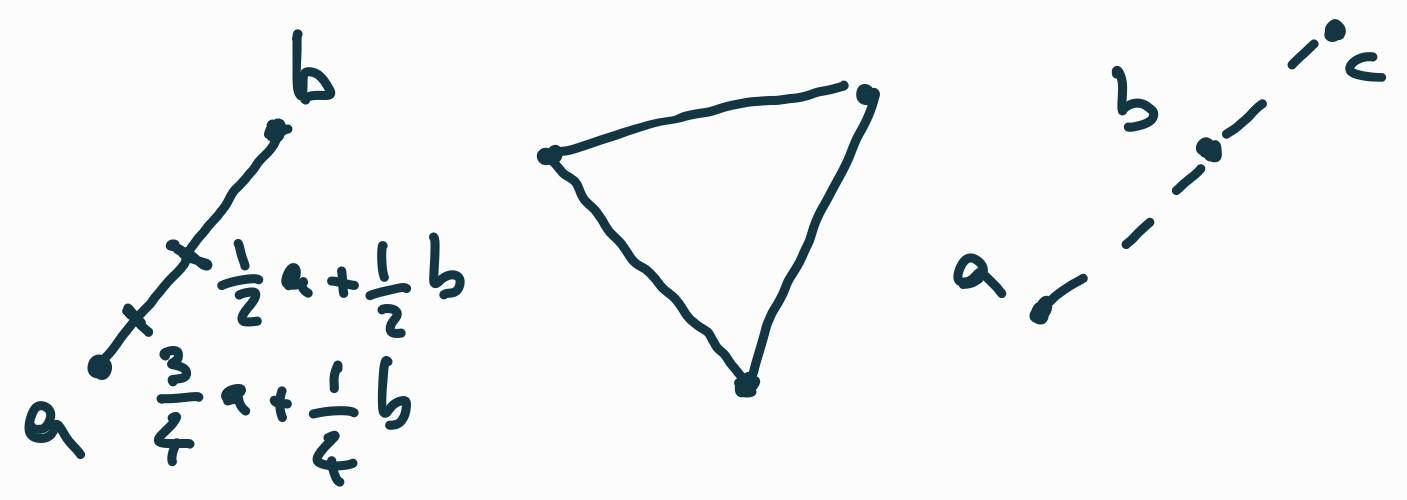
\includegraphics[width=0.5\textwidth]{tempimages/ConvexExamples.jpg}
\end{figure}

\begin{remark}
	In terms of the convex space, all the mixtures between two ensembles correspond to the segment between them; all the mixtures between three ensembles correspond to the triangle formed by the three elements and so on. An ensemble $\ens[a]$ is a component of a different ensemble $\ens[b]$ if the segment connecting $\ens[a]$ and $\ens[b]$ can be extended past $\ens[b]$. If two elements are not a component of each other, then they are the extreme points of the line that connects the two. That is, the segment cannot be extended.
\end{remark}

\begin{figure}[H]
	\centering
	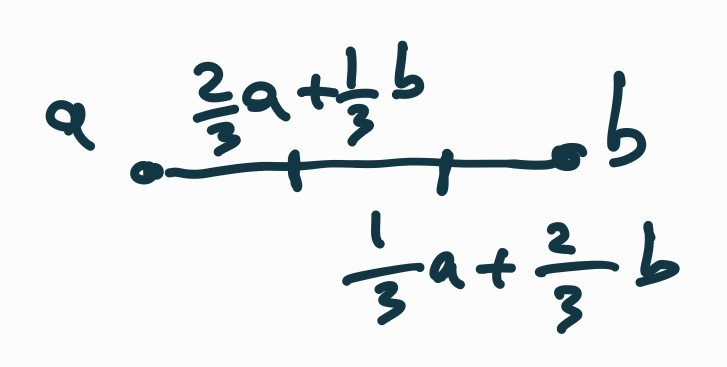
\includegraphics[width=0.4\textwidth]{tempimages/ComponentNotOrder.jpg}
\end{figure}

\begin{remark}
	Note that two ensembles can be components of each other. Consider $\frac{2}{3} \ens[a] + \frac{1}{3} \ens[b]$ and $\frac{1}{3} \ens[a] + \frac{2}{3} \ens[b]$. We can write $\frac{2}{3} \ens[a] + \frac{1}{3} \ens[b] = \frac{1}{2}\left(\frac{1}{3} \ens[a] + \frac{2}{3} \ens[b]\right) + \frac{1}{2} \ens[a]$ and $\frac{1}{3} \ens[a] + \frac{2}{3} \ens[b] = \frac{1}{2}\left(\frac{2}{3} \ens[a] + \frac{1}{3} \ens[b]\right) + \frac{1}{2} \ens[b]$ (they are both midpoints along each other). Therefore a component is not necessarily ``smaller'' or ``better defined'' than the mixture. Mathematically, ``being a component of'' is not a partial order. It is reflexive and transitive, but it is not antisymmetric. In practical terms, we need something else to tell us whether we are, for example, taking a limit with components that become ``smaller and smaller.''
\end{remark}

\begin{defn}
	Let $\Ens$ be an ensemble space and $\ens[a], \ens[b] \in \Ens$. We say that they \textbf{have a common component} if we can find $\ens[c] \in \Ens$, the common component, such that $\ens[a] = p_1 \ens[c] + \bar{p}_1 \ens_1$ and $\ens[b] = p_2 \ens[c] + \bar{p}_2 \ens_2$ for some $\ens_1, \ens_2 \in \Ens$ and $p_1, p_2 \in (0,1]$. Otherwise, we say they \textbf{have no common component}, or are \textbf{separate}, noted $\ens[a] \separate \ens[b]$. Two ensembles have a common component in $A \subseteq \Ens$ if the common component can be found in $A$, and are separate in $A$ if there is none. Two sets of ensembles $A, B \subseteq \Ens$ are separate if all the elements of one are separate from all the elements of the other. That is, $A \separate B$ if $\ens[a] \separate \ens[b]$ for all $\ens[a] \in A$ and $\ens[b] \in B$.
\end{defn}

\begin{figure}[H]
	\centering
	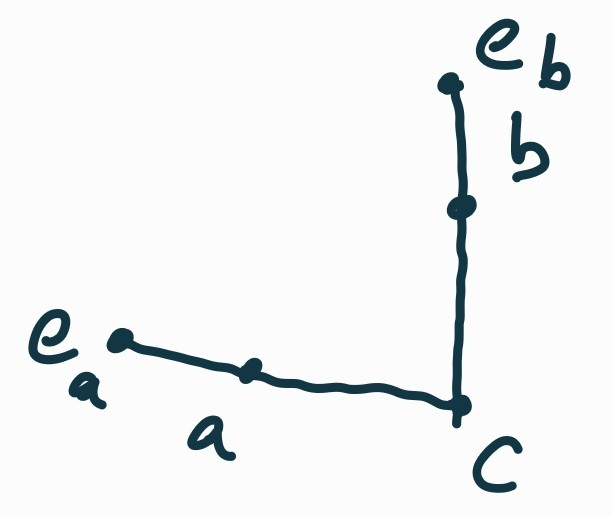
\includegraphics[width=0.3\textwidth]{tempimages/CommonComponent.jpg}
\end{figure}

\begin{remark}
	If two ensembles $\ens[a]$ and $\ens[b]$ have a common component $\ens[c]$, then the ensemble space contains a triangle where $\ens[c]$ is a vertex and $\ens[a]$ and $\ens[b]$ are points on the sides that connect to $\ens[c]$.
\end{remark}

\begin{coro}
	The previous definitions obey the following:
	\begin{enumerate}
		\item every ensemble is a component of itself
		\item if $\ens[a]$ is a component of $\ens[b]$, then $\ens[a]$ and $\ens[b]$ have a common component and therefore they are not separate
		\item separateness is an irreflexive symmetric relation
	\end{enumerate}
\end{coro}

\begin{proof}
	1. Since by idempotence $\ens = p \ens + \bar{p} \ens$ for any $p$, then every ensemble is a mixture of itself, and therefore it is a component of itself.
	
	2. By idempotence, we can write $\ens[a] = p_1 \ens[a] + \bar{p}_1 \ens[a]$ for some $p_1 \in (0,1]$. Since $\ens[a]$ is a component of $\ens[b]$, we can write $\ens[b] = p_2 \ens[a] + \bar{p}_2 \ens[e]_2$ for some $p_2 \in (0, 1]$ and $\ens[c] \in \Ens$. Therefore $\ens[a]$ and $\ens[b]$ have $\ens[a]$ as a common component.
	
	3. Since every ensemble is a component of itself, every ensemble has a common component with itself and therefore is not separate from itself. This proves that separateness is irreflexive. The definition of common component is symmetric and therefore so is separateness.
\end{proof}
\end{mathSection}

Since separateness is defined on top of mixing, it has an important relationship with mixtures: if an ensemble is separate from a mixture of two elements, it is separate from both elements and all their mixtures.

\begin{mathSection}
\begin{prop}[Separateness extends to all mixtures]\label{pm_es_separateExtendsMixtures}
	Let $\ens,\ens_1,\ens_2 \in \Ens$. If $\ens$ has no common component with a mixture of $\ens_1$ and $\ens_2$ then it has no common component with any mixture of $\ens_1$ and $\ens_2$ and with either $\ens_1$ or $\ens_2$. That is, if $\ens \separate p \ens_1 + \bar{p} \ens_2$ for some $p \in (0, 1)$ then $\ens \separate p \ens_1 + \bar{p} \ens_2$ for all $p \in [0, 1]$.
\end{prop}

\begin{figure}[H]
	\centering
	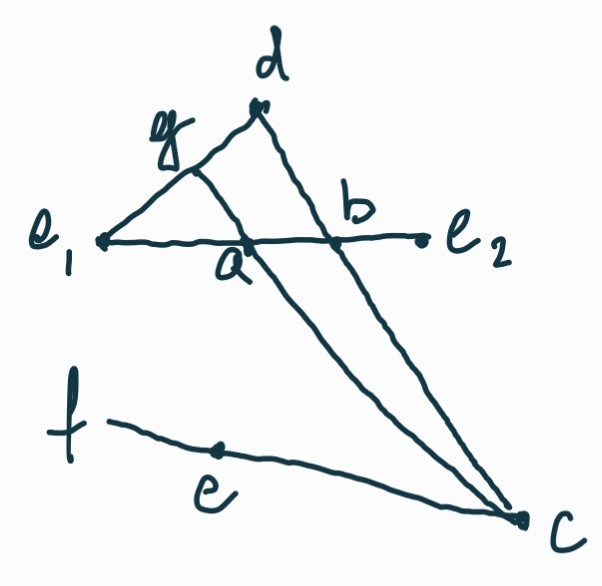
\includegraphics[width=0.3\textwidth]{tempimages/DistinctAndMixture.jpg}
\end{figure}

\begin{proof}
	Let $\ens \separate \ens[a] = p \ens_1 + \bar{p} \ens_2$ for some $p \in (0, 1)$. Let $\ens[b] = \alpha \ens_1 + \bar{\alpha} \ens_2$ with $0 \leq \alpha < p$. Suppose $\ens[b]$ is not separate from $\ens$. Then we can find $\ens[c] \in \Ens$ such that $\ens[b] = \beta \ens[c] + \bar{\beta} \ens[d]$ and $\ens = \gamma \ens[c] + \bar{\gamma} \ens[f]$ for some $\ens[d], \ens[f] \in \Ens$ and $\beta, \gamma \in (0, 1)$.
	
	Setting $\epsilon = \frac{p - \alpha}{\bar{\alpha}}$ and $\lambda = \bar{\epsilon} \beta$ we have:
	\begin{align*}
		\ens[a] &= p \ens_1 + \bar{p} \ens_2 = \left(p - \frac{\bar{p}}{\bar{\alpha}} \alpha \right) \ens_1 + \frac{\bar{p}}{\bar{\alpha}} \alpha \ens_1 + \frac{\bar{p}}{\bar{\alpha}} \bar{\alpha}\ens_2 \\
		&= \left(\frac{p\bar{\alpha} - \bar{p}\alpha}{\bar{\alpha}} \right) \ens_1 + \frac{\bar{p}}{\bar{\alpha}} (\alpha \ens_1 + \bar{\alpha} \ens_2) = \left(\frac{p - p\alpha - \alpha + p \alpha}{\bar{\alpha}} \right) \ens_1 + \frac{1 - p + \alpha - \alpha}{\bar{\alpha}} (\alpha \ens_1 + \bar{\alpha} \ens_2) \\
		&= \frac{p - \alpha}{\bar{\alpha}}  \ens_1 + \left( 1 - \frac{p - \alpha}{\bar{\alpha}}\right) (\alpha \ens_1 + \bar{\alpha} \ens_2) = \epsilon \ens_1 + \bar{\epsilon} (\alpha \ens_1 + \bar{\alpha} \ens_2) = \epsilon \ens_1 + \bar{\epsilon} \ens[b] \\
		&= \epsilon \ens_1 + \bar{\epsilon} ( \beta \ens[c] + \bar{\beta} \ens[d] ) = \bar{\epsilon} \beta \ens[c] + \epsilon \ens_1 + \bar{\epsilon} \bar{\beta} \ens[d] = \lambda \ens[c] + \bar{\lambda} \ens[g]
	\end{align*}
	where $\ens[g] = \frac{1}{\bar{\lambda}}\left( \epsilon \ens_1 + \bar{\epsilon} \bar{\beta} \ens[d] \right)$. This means $\ens[a]$ and $\ens$ have a common component, which is a contradiction. Therefore $\ens \separate \alpha \ens_1 + \bar{\alpha} \ens_2$ for all $\alpha \in [0, p]$.
	
	We can repeat the argument switching $\ens_1$ with $\ens_2$ and find $\ens \separate \alpha \ens_1 + \bar{\alpha} \ens_2$ for all $\alpha \in [0, 1]$.
\end{proof}

\begin{figure}[H]
	\centering
	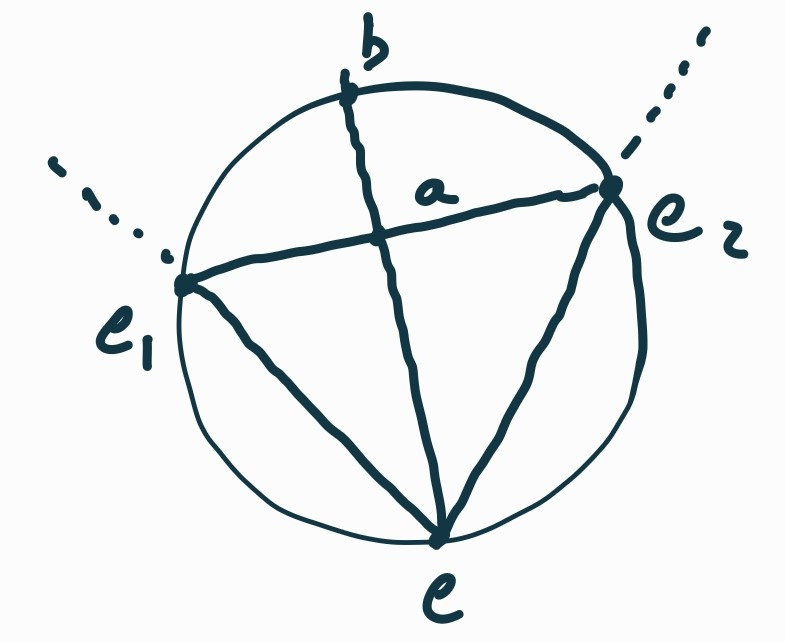
\includegraphics[width=0.3\textwidth]{tempimages/MixturesDoNotPreserveSeparateness.jpg}
\end{figure}

\begin{remark}
	Note that the property does not work the other way around, in the sense that $\ens \separate \ens_1$ and $\ens \separate \ens_2$ does not imply $\ens \separate \alpha \ens_1 + \bar{\alpha} \ens_2$ for all $\alpha \in [0, 1]$. We can find a counterexample in quantum mechanics. Suppose that $\ens$, $\ens_1$ and $\ens_2$ are three pure states within the same two-dimensional subspace. These will be points on the surface of a Bloch ball, which will identify a circle. Since they are pure states, they will be all separate. However, if we take a mixture $\ens[a]$ of $\ens_1$ and $\ens_2$, this can also be written as a mixture of $\ens$ and some $\ens[b]$. Since $\ens$ is a component of $\ens[a]$, they are not separate.
\end{remark}
\end{mathSection}

\subsection{Convex subsets and convex hull}

In many cases, we will need to discuss the set of all possible mixtures of a given set of ensembles. Mathematically, this is the convex closure meaning that we take all possible convex combinations of the given ensembles. Additionally, since the mixture is only a finite operation, we will use the topology to reach all possible limits, all possible infinite mixtures. The topology, in fact, is what defines the limits and will tell us whether a particular infinite convex combination corresponds to a valid mixture or not.

\begin{mathSection}
\begin{defn}
	Let $\Ens$ be an ensemble space. We say $A \subseteq \Ens$ is a \textbf{convex subset} of $\Ens$ if it contains all possible mixtures, including infinite ones, of its elements. Formally, it is a topologically closed set that is also closed under convex combinations. If we want to stress that we are closing only under finite mixing, we say that $A$ is closed under finite convex combination.
\end{defn}

\begin{prop}
	The set $\mathfrak{Conv}_{\Ens}$ of all convex subsets of $\Ens$ ordered by set inclusion is a topped $\bigcap$-structure and therefore is also a complete lattice.
\end{prop}

\begin{proof}
	Let $\mathfrak{Conv}_{\Ens}$ be the set of all convex subsets of $\Ens$ ordered by set inclusion. The empty set $\emptyset \subset \Ens$ is a convex set. The whole space $\Ens \subseteq \Ens$ is also a convex set. Then $\mathfrak{Conv}_{\Ens}$ is therefore a bounded ordered set.
	
	Let $A, B \in \mathfrak{Conv}_{\Ens}$ be two convex subsets. Consider $A \cap B$. Any mixture of elements in $A \cap B$ is both a mixture of elements in $A$ and a mixture of elements in $B$. Therefore any mixture of elements of $A \cap B$ is both an element of $A$ and an element of $B$. This means it is also an element of $A \cap B$, which is therefore a convex set.
	
	The previous argument generalizes to a family of convex subsets $\{A_i\}_{i \in I} \subseteq \mathfrak{Conv}_{\Ens}$. That is, an ensemble is a mixture of elements of $\bigcap_{i \in I} A_i$ if and only if is a mixture of elements of $A_i$ for every $i$. Moreover, the intersection of infinitely many closed sets is still closed. Therefore $\bigcap_{i \in I} A_i \in \mathfrak{Conv}_{\Ens}$ and $\mathfrak{Conv}_{\Ens}$ is an $\bigcap$-structure. This also means that it is a complete lattice. (TODO: find a link to the theorem)
\end{proof}

\begin{defn}
	Let $A \subseteq \Ens$ be a subset of an ensemble space. The \textbf{convex hull} of $A$, noted $\hull(A)$ is the set of all possible mixtures that can be constructed with elements contained in $A$, including infinite ones. Formally, it is the topological closure of the closure of $A$ under convex combination. That is, it is the smallest convex subset that contains $A$.
\end{defn}

\begin{coro}\label{pm_es_hullProp}
	The convex hull has the following properties
	\begin{enumerate}
		\item $A \subseteq \hull(A)$
		\item $A \subseteq B \implies \hull(A) \subseteq \hull(B)$
		\item $\hull(\hull(A)) = \hull(A)$
	\end{enumerate}
	and is therefore a closure operation
\end{coro}

\begin{proof}
	1. Every element of $A$ is trivially a mixture of elements of $A$. Therefore $A \subseteq \hull(A)$.
	
	2. Let $\ens \in \hull(A)$. Then it is a mixture of some elements of $A$. Since $A \subseteq B$, then $\ens$ is also the mixture of some elements of $B$ and therefore $\ens \in \hull(B)$.
	
	3. Since $\hull(\hull(A))$ is the smallest convex subset that contains $\hull(A)$, and since $\hull(A)$ is a convex subset, then $\hull(\hull(A))$ must be $\hull(A)$ since no smaller set can contain all elements of $\hull(A)$.
\end{proof}

\begin{coro}
	A subset $A \subseteq \Ens$ is convex if and only if it is its own convex hull.
\end{coro}

\begin{proof}
	Let $A \subseteq \Ens$ be a convex subset. By \ref{pm_es_hullProp} we have $A \subseteq \hull(A)$. By definition of convex set, we have $\hull(A) \subseteq A$. Therefore $A = \hull(A)$. Conversely, let $A \subseteq \Ens$ be a set of ensembles not necessarily convex. By definition, $\hull(A)$ is closed under mixture and is therefore a convex subset.
\end{proof}

\begin{prop}
	The hull is continuous from above. That is, $\hull(\lim\limits_{i \to \infty} A_i) = \lim\limits_{i \to \infty} \hull(A_i)$ for any decreasing sequence $A_i \subseteq \Ens$.
\end{prop}

\begin{proof}
	Since $A_i$ is a decreasing sequence, $\lim\limits_{i \to \infty} A_i = \bigcap_i A_i$. Also, since $A_{i+1} \subseteq A_i$, then $\hull(A_{i+1}) \subseteq \hull(A_i)$ and therefore $\hull(A_i)$ is a decreasing sequence. This also means $\lim\limits_{i \to \infty} \hull(A_i) = \bigcap_i \hull(A_i)$. Therefore we need to show that $\hull(\bigcap_i A_i) = \bigcap_i \hull(A_i)$.
	
	Since the arbitrary intersection of convex sets is a convex set, $\bigcap_i \hull(A_i)$ is a convex set. Therefore $\bigcap_i \hull(A_i) = \hull(\bigcap_i \hull(A_i))$. Note that a mixture of mixture of elements can always be re-expressed as a mixture of elements. Moreover, an element that is the mixture of $A_i$ for all $i$ can be re-expressed as a mixture of the common elements, since $A_{i+1} \subset A_i$. Therefore $\hull(\bigcap_i \hull(A_i)) = \hull(\bigcap_i A_i)$. This means $\hull(\bigcap_i A_i) = \bigcap_i \hull(A_i)$, which proves the proposition.
\end{proof}

\begin{remark}
	Note that the hull is not necessarily continuous from below. That is, it is not necessarily true that $\hull(\lim\limits_{i \to \infty} A_i) = \lim\limits_{i \to \infty} \hull(A_i)$ for any increasing sequence $A_i \subseteq \Ens$. The limit from below, in fact, would correspond to the infinite union of closed sets, which is not necessarily a closed set. Therefore if we take the closure after the limit, we are going to include the infinite convex combinations that require, for example, an element from each of the $A_i$.
\end{remark}
\end{mathSection}

\begin{conj}
	The topological closure of the finite convex closure is closed under convex combinations.
\end{conj}

\begin{proof}
	Using the axiom of entropy, we know that the ensemble space embeds in a vector space. If we are able to show that it embeds in a topological vector space, then we are taking the closure of a convex subset of a topological vector space. It should be a property that the convex closure should be in the same subspace of the one generated by the convex set. Therefore all limit points would can be generate as limits of elements of the convex set.
\end{proof}

\section{Axiom of entropy}

The third and final property of ensembles is that they have a well-defined entropy. The entropy quantifies the variability of the elements within the ensembles. That is, since an ensemble represents all possible preparations of equivalent systems prepared according to the same procedure, we are asking how much those preparations are different from each other. No matter what the full description of each individual preparation may be, we can assume that their variability has some specific features. It will have to be compatible with experimental verifiability (i.e. the variability must be a continuous function with respect to the topology) and with statistical mixing (i.e. the variability cannot decrease during mixing and it maximally increases when the ensembles do not overlap). The formula for entropy can then be recovered with these very broad physically justified assumptions.

\begin{mathSection}
\begin{axiom}[Axiom of entropy]
	Every element of the ensemble is associated with an \textbf{entropy} which quantifies the variability of the preparations of the ensemble. Formally, an ensemble space $\Ens$ is equipped with a function $S : \Ens \to \mathbb{R}$, defined up to a positive multiplicative constant representing the unit numerical value. The entropy has the following properties:
	\begin{itemize}
		\item \textbf{Continuity}\footnote{Currently, we are imposing that the entropy is continuous. There may be a chance that this requirement is redundant, as strict concavity and the upper variability bound may already impose this. We have found proofs that show that real valued convex/concave functions of real values are continuous. These proofs fail at the extreme points, but the upper variability bound may fix this. Another open question is whether differentiability is also an independent requirement.}
		\item \textbf{Strict concavity}: $S(p\ens[a] + \bar{p} \ens[b]) \geq p S(\ens[a]) + \bar{p} S(\ens[b])$ with the equality holding if and only if $\ens[a] = \ens[b]$
		\item \textbf{Upper variability bound}: there exists a universal function $I(p_1, p_2)$ (i.e. the same for all ensemble spaces) such that $S(p\ens[a] + \bar{p} \ens[b]) \leq I(p, \bar{p}) + p S(\ens[a]) + \bar{p} S(\ens[b])$; if the equality holds, $\ens[a]$ and $\ens[b]$ are \textbf{non-overlapping} or \textbf{orthogonal}, noted $\ens[a] \ortho \ens[b]$
		\item \textbf{Mixtures preserve orthogonality}:\footnote{It is unclear whether ``mixtures preserve orthogonality'' is an independent axiom. Intuitively, the following argument tells us that it is. Take the 2 dimensional simplex (i.e. a triangle) that represents a classical discrete probability space over three elements. Take the standard entropy, which will satisfy ``mixtures preserve orthogonality''. This is because the middle point has entropy $\log 3$. We can imagine redefining the entropy so that it is a little bit lower in the center but it is unchanged on the sides. However, one needs to provide an actual example and show that it satisfies all axioms. It may also be that only one direction is an independent axiom. That is, that orthogonality with the components implies orthogonality with the mixtures. This is what does not hold for separateness.} $\ens[a] \ortho \ens[b]$ and $\ens[a] \ortho \ens[c]$ if and only if $\ens[a] \ortho p \ens[b] + \bar{p} \ens[c]$ for any $p \in (0,1)$
	\end{itemize}
\end{axiom}

\begin{justification}
	The entropy quantifies the variability of the instances of the ensemble. Since the ensemble represents a collection of preparations of equivalent systems, and since each instance will in general be potentially different, it is legitimate to ask how much variability there is among the different instances. We are assuming that the entropy is a quantity (i.e. a linearly ordered property), meaning that it is always meaningful to tell whether one ensemble has more variability than another. If this is the case, the later requirements of continuity and strict concavity will force the entropy to be a real valued quantity. This is because the variability will change under statistical mixtures, and since statistical mixtures are performed with real valued coefficients, the variability will have to be a real valued quantity. Whether it is conceptually possible to have a characterization of variability that is not linearly ordered but still have a meaningful connection with statistical mixing is an open question, therefore we are not able to fully justify entropy's linear ordering at this time. Therefore the linear ordering of the entropy should be considered an assumption. Provided that assumption, we are justified to assume the existence of a real valued function that returns the entropy, a measure of variability of the ensemble.
	
	Since the entropy is a real valued quantity, it will have a corresponding unit. This unit is independent from all other units, and therefore the overall structure of the ensemble space must be independent of this choice. Mathematically, the physical dimension of the unit is not captured, just its numeric value. A change of unit may change the numeric value by a multiplicative constant. Since variability is an ordered quantity, we want the change of units to respect the ordering and therefore it should be a positive multiplicative constant. This justifies that the entropy function is defined up to a positive multiplicative constant.
	
	Note that the additivity of the entropy over independent systems fixes the absolute scale. If $S_{AB} = S_A + S_B$, in fact, one can't rescale all three terms by an additive factor and preserve the relationship.
	
	The variability, in the end, will have physical consequences, and it will therefore be measurable, thus experimentally verifiable: it will have to be a topologically continuous function. Moreover, small changes in the ensemble should produce small changes in the variability, which justifies analytical continuity. We are therefore justified to assume continuity of the entropy.
	
	Suppose we have two ensembles and we perform a statistical mixture. There are going to be three sources of variability: the two ensembles and the random choice at every instance. The total contribution from the original ensembles will be the average variability of the original ensembles. This is increased by the variability introduced by the random choice, which is always a positive contribution. Therefore the final variability cannot be less than the average of the original ensembles. That is, $S(p\ens[a] + \bar{p} \ens[b]) \geq p S(\ens[a]) + \bar{p} S(\ens[b])$. If we are mixing an ensemble with itself, this is equivalent to just choosing from the original ensemble, therefore the variability will not increase. Conversely, if the variability stays the same, it means that the random choice does not increase the variability, and therefore we must be choosing between equivalent ensembles. Therefore we are justified to assume that entropy is strictly concave.
	
	On the other hand, the variability cannot increase arbitrarily during mixture. The maximum variability will be given when the two ensembles are non-overlapping, when an instance of the first ensemble cannot be produced by the second ensemble. That is, a single instance is enough to determine whether we have the first ensemble or the second. In this case, the variability is increased by the variability of the random choice, which must depend only on the mixture coefficient, and not the nature of the ensembles themselves. That is, $S(p\ens[a] + \bar{p} \ens[b]) \leq I(p, \bar{p}) + p S(\ens[a]) + \bar{p} S(\ens[b])$ is the upper variability bound, which is saturated if and only if the $\ens[a]$ and $\ens[b]$ are non-overlapping. The actual function $I$ is left unspecified and, as we show in proposition \ref{pm_es_entropyUnique}, it will correspond to the Shannon entropy as it is the only indicator of variability that will satisfy the axiom of entropy. This justifies the upper variability bound.
	
	Now suppose ensemble $\ens[a]$ is non-overlapping with $\ens[b]$ and $\ens[c]$. That is, an instance of $\ens[a]$ cannot ever be produced by either $\ens[b]$ or $\ens[c]$. Then an instance of $\ens[a]$ cannot be produced by a mixture of $\ens[b]$ and $\ens[c]$, since ultimately a mixture of $\ens[b]$ and $\ens[c]$ will return an instance of one of the two. Therefore $\ens[a]$ is non-overlapping with any mixture of $\ens[b]$ and $\ens[c]$. The argument works in reverse as well: if an instance of $\ens[a]$ cannot be produced by a mixture of $\ens[b]$ and $\ens[c]$, then it cannot be produced by either. This justifies mixtures preserve orthogonality.
\end{justification}
\end{mathSection}

We should now verify that the axiom of entropy is satisfied by the standard cases.

\begin{mathSection}
	\begin{prop}
		Discrete classical ensemble spaces, continuous classical ensemble spaces and quantum ensemble spaces satisfy the axiom of entropy.
	\end{prop}
	
	\begin{proof}
		Let's first look at the classical continuous case. Every ensemble is represented by a distribution $\rho(x)$ with $\int_X \rho(x) d\mu=1$. The entropy is given by $S(\rho) = - \int_X \rho \log \rho d\mu$. This is a continuous function of $\rho$.
		
		\begin{figure}[H]
			\centering
			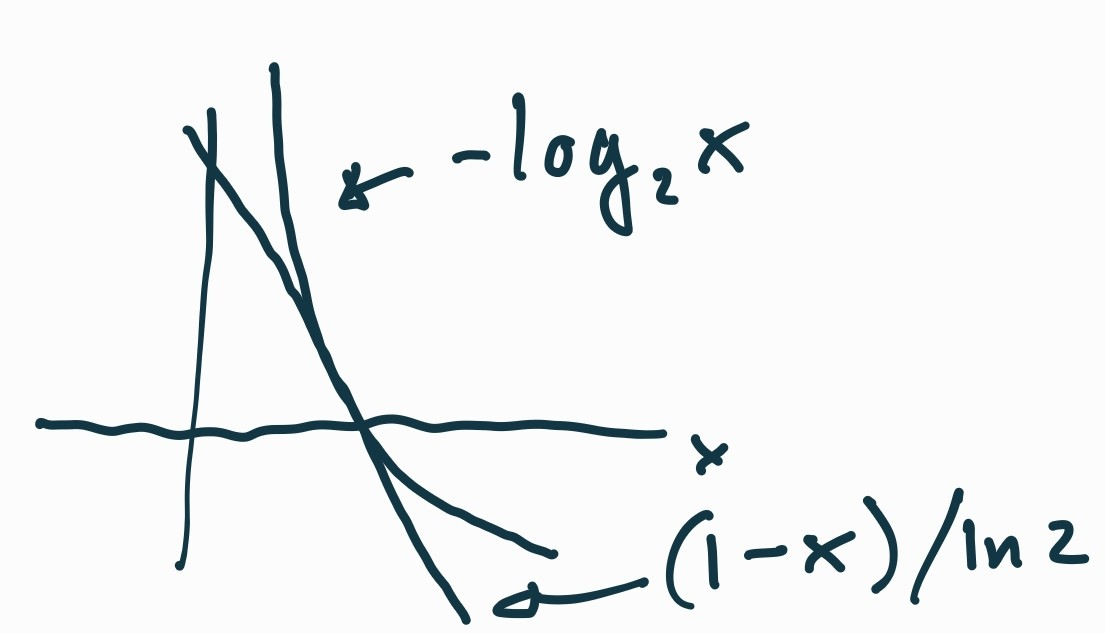
\includegraphics[width=0.5\textwidth]{tempimages/LogBound.jpg}
		\end{figure}
		
		To show strict concavity, note that $- \log x \geq \frac{1-x}{\ln 2}$ with the equality holding if and only if $x=1$. We have
		\begin{equation}
			\begin{aligned}
				S(p\rho_1 + \bar{p}\rho_2) &= - \int_X \left(p\rho_1 + \bar{p}\rho_2\right) \log \left(p\rho_1 + \bar{p}\rho_2\right) d\mu \\
				&= - \int_X p\rho_1 \log \left(p\rho_1 + \bar{p}\rho_2\right) d\mu - \int_X \bar{p}\rho_2 \log \left(p\rho_1 + \bar{p}\rho_2\right) d\mu \\
				&= - \int_X p\rho_1 \log \frac{p\rho_1 + \bar{p}\rho_2}{\rho_1} d\mu - \int_X p\rho_1 \log \rho_1 d\mu \\
				&- \int_X \bar{p}\rho_2 \log \frac{p\rho_1 + \bar{p}\rho_2}{\rho_2} d\mu - \int_X \bar{p}\rho_2 \log \rho_2 d\mu \\
				&\geq \int_X p\rho_1 \frac{1}{\ln 2} \left(1 - \frac{p\rho_1 + \bar{p}\rho_2}{\rho_1} \right)   d\mu - p \int_X \rho_1 \log \rho_1 d\mu \\
				&+ \int_X \bar{p}\rho_2 \frac{1}{\ln 2} \left(1 - \frac{p\rho_1 + \bar{p}\rho_2}{\rho_2} \right)   d\mu - \bar{p} \int_X \rho_2 \log \rho_2 d\mu \\
				&= \frac{p}{\ln 2}\left[ \int_X \rho_1 d\mu - \int_X \left(p\rho_1 + \bar{p}\rho_2\right) d\mu  \right] + p S(\rho_1) \\
				&+ \frac{\bar{p}}{\ln 2}\left[ \int_X \rho_2 d\mu - \int_X \left(p\rho_1 + \bar{p}\rho_2\right) d\mu  \right] + \bar{p} S(\rho_2) \\
				&= \frac{p}{\ln 2}\left[ 1 - 1  \right] + p S(\rho_1) + \frac{\bar{p}}{\ln 2}\left[ 1 - 1 \right] + \bar{p} S(\rho_2) \\
				&= p S(\rho_1) + \bar{p} S(\rho_2) \\
			\end{aligned}
		\end{equation}
		The equality holds if and only if $\frac{p\rho_1 + \bar{p}\rho_2}{\rho_1} = 1$ which is exactly when $\rho_1 = \rho_2$.
		
		
		\begin{figure}[H]
			\centering
			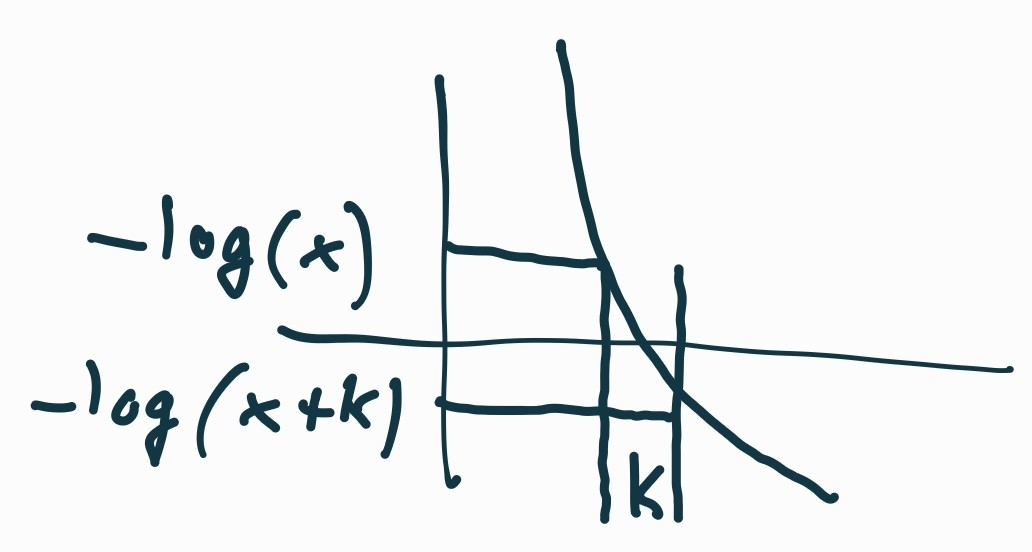
\includegraphics[width=0.5\textwidth]{tempimages/LogMonotone.jpg}
		\end{figure}
		For the upper bound, note that the logarithm is a strictly increasing function, and therefore $- \log(x + k) \leq -\log(x)$ for any $k \geq 0$, with equality holding if and only if $k=0$. We have
		\begin{equation}
			\begin{aligned}
				S(p\rho_1 + \bar{p}\rho_2) &= - \int_X \left(p\rho_1 + \bar{p}\rho_2\right) \log \left(p\rho_1 + \bar{p}\rho_2\right) d\mu \\
				&= - \int_X p\rho_1 \log \left(p\rho_1 + \bar{p}\rho_2\right) d\mu - \int_X \bar{p}\rho_2 \log \left(p\rho_1 + \bar{p}\rho_2\right) d\mu \\
				&\leq  - \int_X p\rho_1 \log p\rho_1 d\mu - \int_X \bar{p}\rho_2 \log \bar{p}\rho_2 d\mu\\
				&=  - \int_X p\rho_1 \log p d\mu - \int_X p\rho_1 \log \rho_1 d\mu - \int_X \bar{p}\rho_2 \log \bar{p} d\mu - \int_X \bar{p}\rho_2 \log \rho_2 d\mu\\
				&=  - p \log p \int_X \rho_1 d\mu - p \int_X \rho_1 \log \rho_1 d\mu - \bar{p} \log \bar{p} \int_X \rho_2 d\mu - \bar{p} \int_X \rho_2 \log \rho_2 d\mu\\
				&=  - p \log p - \bar{p} \log \bar{p} + p S(\rho_1) + \bar{p} S(\rho_2)\\
			\end{aligned}
		\end{equation}
		The equality holds if and only if $\rho_2=0$ wherever $\rho_1\neq0$ and $\rho_1=0$ wherever $\rho_2\neq0$. That is, the equality holds if and only if the two distributions have disjoint support. Therefore orthogonal distributions are exactly distributions with disjoint support.
		
		Suppose $\rho_4$ has disjoint support from $\rho_1 = p \rho_2 + \bar{p} \rho_3$, then it has disjoint support from $\rho_2$ and $\rho_3$ because the support of $\rho_1$ is the union of the supports of $\rho_2$ and $\rho_3$. Conversely, if $\rho_4$ has disjoint support from both $\rho_2$ and $\rho_3$, then $\rho_4$ has disjoint support from $\rho_1$ as well. Therefore mixtures preserve orthogonality.
		
		All these arguments are valid for discrete classical ensemble spaces, changing integrals to sums.
		
		For the quantum case, we haven't found a short proof that does not require defining the KL divergence and the entropy for a joint distribution. The result, however, is generally known and can be found, for example, in \href{https://www.cambridge.org/highereducation/books/quantum-computation-and-quantum-information/01E10196D0A682A6AEFFEA52D53BE9AE}{Nielsen-Chuang}.
	\end{proof}
\end{mathSection}


\subsection{Uniqueness of entropy of mixing coefficients}

We now prove that the function $I(p,\bar{p})$ must be the Shannon entropy.

\begin{mathSection}
\begin{thrm}[Uniqueness of entropy]\label{pm_es_entropyUnique}
	The entropy of the coefficients $I(p,\bar{p})$ is the Shannon entropy. That is, $I(p,\bar{p}) = - \kappa \left(p \log p + \bar{p} \log \bar{p}\right)$ where $\kappa>0$ is the arbitrary multiplicative constant for the entropy. For a mixture of arbitrarily many elements, $I(\{p_i\}) = - \kappa \sum_i p_i \log p_i$.
\end{thrm}

\begin{proof}
	Since the upper entropy bound has to be the same for all spaces, let us assume that $\Ens$ is such that it contains countably many orthogonal ensembles $\{\ens_l\}_{l=1}^{\infty}$. Since mixtures preserve orthogonality, for any convex combinations $\sum_i p_i \ens[a]_i$ of finitely many $\{\ens[a]_i\}_{i=1}^{n} \subset \{\ens_l\}_{l=1}^{\infty}$,  we have $S(\sum_i p_i \ens[a]_i ) = I_n(p_1, p_2, \dots, p_n) + \sum_i p_i S(\ens[a]_i)$ where $I_n : \mathbb{R}^n \to \mathbb{R}$ is a function of the coefficients only. Note that, given commutativity, the order of the $p_i$ does not matter and, since the coefficients can be zero, we must have $I_n(p_1, p_2, \dots, p_n) = I_{n+1}(p_1, p_2, \dots, p_n, 0)$. Therefore we can think of $I$ as a function of the coefficients and write $I(\{p_i\}_{i=1}^{n})$.
	
	We now show that $I\left(\left\{\frac{1}{n}\right\}_{i=1}^{n}\right) = \kappa \log n$ with $\kappa > 0$. That is, the maximum increase of entropy for a uniform distribution is proportional to the logarithm of the number of cases. Pick two positive integers $n, m \in \mathbb{Z}^+$. Pick $nm$ elements $\ens[a]_{jk} \in \{e_l\}_{l=1}^{\infty}$ where $1\leq j \leq n$ and $1 \leq  k \leq m$. We have:
	\begin{equation}
		\begin{aligned}
			S\left(\sum_{j=1}^{n}\sum_{k=1}^{m} \frac{1}{n}\frac{1}{m} \ens[a]_{jk}\right) &= I\left(\left\{ \frac{1}{n}\frac{1}{m}\right\}_{i=1}^{nm}\right) + \sum_{j=1}^{n}\sum_{k=1}^{m} \frac{1}{n}\frac{1}{m} S\left(\ens[a]_{jk}\right) \\
			= S\left(\sum_{j=1}^{n} \frac{1}{n} \sum_{k=1}^{m} \frac{1}{m} \ens[a]_{jk}\right)  &=I\left(\left\{ \frac{1}{n}\right\}_{i=1}^{n}\right) + \sum_{j=1}^{n} \frac{1}{n} S\left(\sum_{k=1}^{m}\frac{1}{m}\ens[a]_{jk}\right) \\
			&=I\left(\left\{ \frac{1}{n}\right\}_{i=1}^{n}\right) + \sum_{j=1}^{n} \frac{1}{n}\left(I\left(\left\{ \frac{1}{m}\right\}_{i=1}^{m}\right) +  \sum_{k=1}^{m}\frac{1}{m}S\left(\ens[a]_{jk}\right)\right) \\
			&=I\left(\left\{ \frac{1}{n}\right\}_{i=1}^{n}\right) + I\left(\left\{ \frac{1}{m}\right\}_{i=1}^{m}\right) + \sum_{j=1}^{n} \sum_{k=1}^{m}\frac{1}{n}\frac{1}{m}S\left(\ens[a]_{jk}\right).
		\end{aligned}
	\end{equation}
	Therefore
	\begin{equation}
		\begin{aligned}
			I\left(\left\{ \frac{1}{nm}\right\}_{i=1}^{nm}\right) &=I\left(\left\{ \frac{1}{n}\right\}_{i=1}^{n}\right) + I\left(\left\{ \frac{1}{m}\right\}_{i=1}^{m}\right).
		\end{aligned}
	\end{equation}
	Note that $f(n) = I\left(\left\{ \frac{1}{n}\right\}_{i=1}^{n}\right)$ is a function of $n$ only, such that $f(nm) = f(n) + f(m)$. Since $f$ is continuous, we have $f(n) = \kappa \log n$. Since the entropy is strictly concave, $\kappa$ must be positive. Therefore
	\begin{equation}
		I\left(\left\{ \frac{1}{n}\right\}_{i=1}^{n}\right) = \kappa \log n
	\end{equation}
	for some $\kappa>0$.
	
	We now show that if the coefficients $p_i$ are rationals, $I_n\left(\left\{ p_i\right\}_{i=1}^{n}\right) = - \kappa \sum_{i=1}^{n} p_i \log p_i$. Let $\{p_i\}_{i=1}^{n}$ be rational coefficients for a convex combination. We can write them as $p_i = \frac{m_i}{m}$ where $\{m_i\}, m \in \mathbb{Z}^+$ and $m$ is the least common denominator. Since $p_i$ are the coefficients of a convex combination, we must have $\sum_{i=1}^{n} m_i = m$. Since $m_i$ is a positive integer, we can write $m_i = \sum_{j=1}^{m_i} 1$. We now take $m$ orthogonal ensembles $\ens[a]_{ij}$ where $1 \leq i \leq n$ and $1 \leq j \leq m_i$. We have
	\begin{equation}
		\begin{aligned}
			S\left(\sum_{i=1}^{n}\sum_{j=1}^{m_i} \frac{1}{m} \ens[a]_{ij}\right) &= I\left(\left\{ \frac{1}{m}\right\}_{i=1}^{m}\right) + \sum_{i=1}^{n}\sum_{j=1}^{m_i} \frac{1}{m} S\left(\ens[a]_{ij}\right) \\
			&= \kappa \log m + \sum_{i=1}^{n}\sum_{j=1}^{m_i} \frac{1}{m} S\left(\ens[a]_{ij}\right) \\
		\end{aligned}
	\end{equation}
	\begin{equation}
		\begin{aligned}
			= S\left(\sum_{i=1}^{n} \frac{m_i}{m} \sum_{j=1}^{m_i} \frac{1}{m_i} \ens[a]_{ij}\right)  &=I\left(\left\{ \frac{m_i}{m}\right\}_{i=1}^{n}\right) + \sum_{i=1}^{n} \frac{m_i}{m}  S\left(\sum_{j=1}^{m_i} \frac{1}{m_i} \ens[a]_{ij}\right) \\
			&=I\left(\left\{ p_i\right\}_{i=1}^{n}\right) + \sum_{i=1}^{n} \frac{m_i}{m}\left(I\left(\left\{ \frac{1}{m_i}\right\}_{i=1}^{m_i}\right) + \sum_{j=1}^{m_i} \frac{1}{m_i} S\left(\ens[a]_{ij}\right)\right) \\
			&=I\left(\left\{ p_i\right\}_{i=1}^{n}\right) + \sum_{i=1}^{n} \frac{m_i}{m} I\left(\left\{ \frac{1}{m_i}\right\}_{i=1}^{m_i}\right) + \sum_{i=1}^{n} \frac{m_i}{m} \sum_{j=1}^{m_i} \frac{1}{m_i}S\left(\ens[a]_{ij}\right) \\
			&=I\left(\left\{ p_i\right\}_{i=1}^{n}\right) + \sum_{i=1}^{n} p_i \kappa \log m_i + \sum_{i=1}^{n}  \sum_{j=1}^{m_i} \frac{1}{m} S\left(\ens[a]_{ij}\right).
		\end{aligned}
	\end{equation}
	Therefore
	\begin{equation}
		\begin{aligned}
			\kappa \log m &= I\left(\left\{ p_i\right\}_{i=1}^{n}\right) + \sum_{i=1}^{n} p_i \kappa \log m_i \\
			I\left(\left\{ p_i\right\}_{i=1}^{n}\right) &= \kappa \log m - \sum_{i=1}^{n} p_i \kappa \log m_i = \sum_{i=1}^{n} p_i \kappa \log m - \sum_{i=1}^{n} p_i \kappa \log m_i \\
			&= - \sum_{i=1}^{n} p_i \kappa \log \frac{m_i}{m} = - \kappa \sum_{i=1}^{n} p_i \log p_i.
		\end{aligned}
	\end{equation}
	
	Lastly, let $\{p_i\}_{i=1}^{n}$ be coefficients for a convex combination, not necessarily rational. Since $I$ is continuous and $p_i$ can be approximated with rational values to an arbitrary level of precision, we will have $I\left(\left\{ p_i\right\}_{i=1}^{n}\right) = - \kappa \sum_{i=1}^{n} p_i \log p_i$. In the case of $n=2$, we have $I(p_1, p_2) = - \kappa p_1 \log p_1 - \kappa p_2 \log p_2$.	
\end{proof}

\begin{coro}
	The unit for the entropy is determined (up to the physical dimension) by the maximum of the entropy of the coefficients $I\left(\frac{1}{2}, \frac{1}{2}\right)$. If the entropy is measured in bits, then $I\left(\frac{1}{2}, \frac{1}{2}\right) = 1$.
\end{coro}

\begin{proof}
	A rescaling of the entropy will also rescale the entropy of the coefficients. Therefore setting the value of the maximum of $I$ will set the arbitrary multiplicative factor. If $I\left(\frac{1}{2}, \frac{1}{2}\right) = 1$, then $\kappa$ is equal to one and the logarithm is base two, which corresponds to the entropy measured in bits. Note that this does not fix the physical dimensions of the entropy, only the numerical value.
\end{proof}
\end{mathSection}

\subsection{Separateness and orthogonality}

Separateness and orthogonality are tightly related to each other. First of all, orthogonality implies separateness and is therefore a stronger property. Moreover, orthogonality is an irreflexive symmetric relation, like separateness.

\begin{mathSection}
\begin{prop}
	Orthogonality satisfies the following properties:
	\begin{enumerate}
		\item irreflexivity: $\ens[a] \northo \ens[a]$
		\item symmetry: $\ens[a] \ortho \ens[b]$ if and only if $\ens[b] \ortho \ens[a]$
		\item components are not orthogonal: if $\ens[b]$ is a component of $\ens[a]$ then $\ens[a] \northo \ens[b]$
		\item orthogonality implies separateness: if $\ens[a] \ortho \ens[b]$ then $\ens[a] \separate \ens[b]$.
	\end{enumerate}
\end{prop}

\begin{proof}
	For 1, let $\ens[a] \in \Ens$. We have $S(p\ens[a] + \bar{p}\ens[a]) = S(\ens[a]) < I(p,\bar{p}) + p S(\ens[a]) + \bar{p} S(\ens[a])$. Therefore $\ens[a]$ is not orthogonal to itself as it does not saturate the upper bound.
	
	For 2, note that the upper entropy bound is symmetric in $\ens[a]$ and $\ens[b]$.
	
	For 3, let $\ens[a] = p \ens[b] + \bar{p} \ens[c]$. Since mixtures preserve orthogonality, $\ens[b] \ortho \ens[a]$ if and only if $\ens[b] \ortho \ens[b]$ and $\ens[b] \ortho \ens[c]$. But $\ens[b]$ is not orthogonal to itself, therefore $\ens[a]$ and $\ens[b]$ are not orthogonal.
	
	For 4, we demonstrate the contrapositive: that ensembles that are not separate are not orthogonal. Let $\ens[a], \ens[b] \in \Ens$ have a common component. That is, $\ens[a] = p \ens[c] + \bar{p} \ens[d]$ and $\ens[b] = \lambda \ens[c] + \bar{\lambda} \ens[e]$. Since mixtures preserve orthogonality, $\ens[a] \ortho \ens[b]$ if and only if $\ens[a] \ortho \ens[c]$ and $\ens[a] \ortho \ens[e]$. But $\ens[c]$ is a component of $\ens[a]$, therefore they are not orthogonal. Therefore two ensembles that have a common component are not orthogonal. This means that if two ensembles are orthogonal they cannot have a common component and are therefore separate.
\end{proof}

As we did for separateness, we extend the notion of orthogonality to sets of ensembles.

\begin{defn}
	Two sets of ensembles are orthogonal if all the elements of one are orthogonal to all the elements of the other. That is, $A \ortho B$ with $A, B \subseteq \Ens$ if $\ens[a] \ortho \ens[b]$ for all $\ens[a] \in A$ and $\ens[b] \in B$. 
\end{defn}

\begin{prop}
	Let $A, B \subseteq \Ens$ be two sets of ensembles such that $A \ortho B$. Then the following are true:
	\begin{enumerate}
		\item the two sets are separate: $A \separate B$
		\item their hulls are orthogonal: $\hull(A) \ortho \hull(B)$
	\end{enumerate}
\end{prop}

\begin{proof}
	For 1, by definition $\ens[a] \ortho \ens[b]$ for all $\ens[a] \in A$ and $\ens[b] \in B$. Since orthogonality implies separateness, we also have $\ens[a] \separate \ens[b]$.
	
	For 2, since mixtures preserve orthogonality, every mixture of $A$ is orthogonal to every mixture of $B$. To show that this extends to the closure, let $\ens[a]_i \in A$ and $\ens[b]_j \in B$ be two sequences of finite mixtures that converge in $A$ and $B$ respectively. Consider $f(p,\ens[a]_i, \ens[b]_j) = S(p \ens[a]_i + \bar{p} \ens[b]_j) - p S(\ens[a]_i) - \bar{p} S(\ens[b]_j)$. Since all mixtures are orthogonal, $f(p,\ens[a]_i, \ens[b]_j) = I(p,\bar{p})$. Note that $f$ is a continuous function, therefore the limits will also converge to $I(p,\bar{p})$. This means that every element in the hull of $A$ is orthogonal to every element in the hull of $B$.
\end{proof}
\end{mathSection}

\section{Entropic constraints on the space}

The axiom of entropy not only constrains the functional form of the entropy, but it also constrains the type of space we can have. Additionally, it rules out some spaces that would seem physically pathological.

The entropic structure, in general, will constrain both the topological structure, making it metrizable, and the convex structure, making it embeddable in a vector space. The entropy is also responsible for all the geometric structure of the ensemble space.

\subsection{EXPERIMENTAL: Space of differences}

\begin{defn}
	Given an ensemble space, a difference between two ensemble represents the change required to transform one ensemble into another. Formally, an \textbf{ensemble difference}, or simply a difference, is an ordered pair of ensembles $\ens[a],\ens[b] \in \Ens$, noted $\ens[b] - \ens[a]$. Given a difference $\ens[b] - \ens[a]$, its \textbf{opposite} $-(\ens[b] - \ens[a])$, if it exists, is the pair $\ens[c] - \ens[a]$ where $\frac{1}{2}\ens[b] + \frac{1}{2} \ens[c] = \ens[a]$. Given $k \in [0,1]$, the \textbf{shrunk difference} is defined to be $k(\ens[b] - \ens[a]) = (k\ens[b] + \bar{k}\ens[a]) - \ens[a]$. Given $k \in (1,+\infty)$, a \textbf{stretched difference} $k(\ens[b] - \ens[a])$, if it exists, is a difference $\ens[c] - \ens[a]$ such that $\ens[b] = \frac{1}{k} \ens[c] - \overline{\frac{1}{k}}\ens[a]$. Given two differences $\ens[b] - \ens[a]$ and $\ens[c] - \ens[a]$ with an equal second term, the \textbf{average difference} is defined as $\frac{1}{2}(\ens[b] - \ens[a]) + \frac{1}{2}(\ens[c] - \ens[a]) =\frac{1}{2}(\ens[b] + \ens[c]) - \ens[a]$.
\end{defn}

\begin{figure}[h]
	\centering
	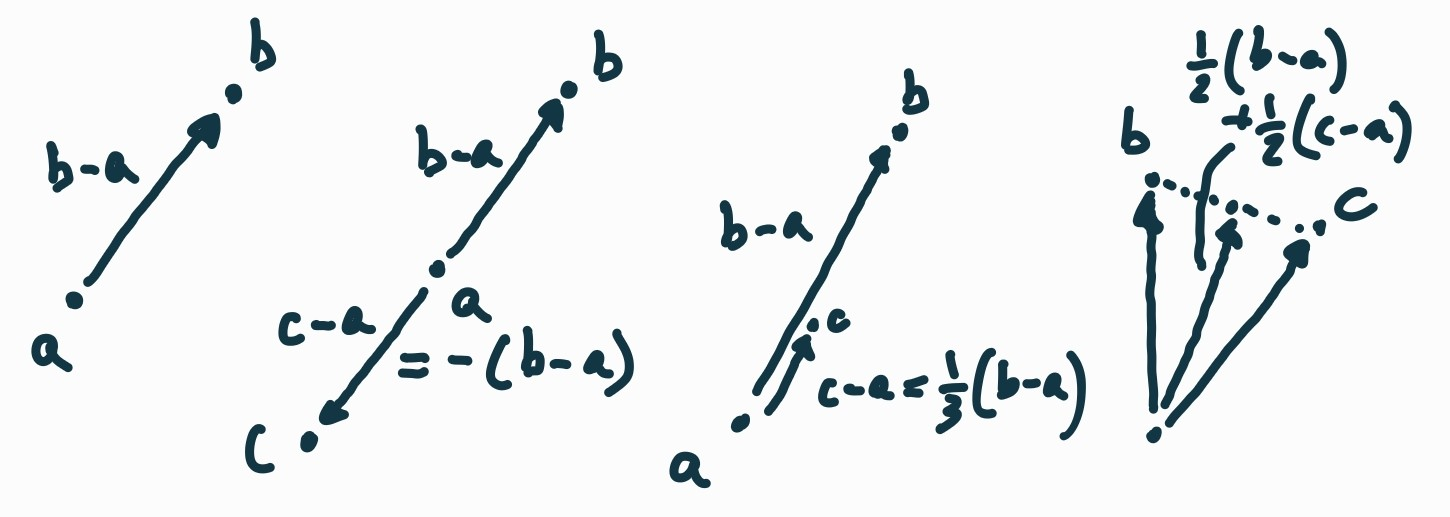
\includegraphics[width=0.7\textwidth]{tempimages/EnsembleDifferences.jpg}
	\caption{This picture represent the motivation of the definition of the operations on the space of differences.}
\end{figure}

\begin{remark}
	Note that the notation is chosen so that, effectively, we can simply manipulate differences as if we have operations on the actual ensembles. For example $k(\ens[b] - \ens[a]) = k\ens[b] - k \ens[a] = k\ens[b] - k \ens[a] + \ens[a] - \ens[a] = k\ens[b] + (1 - k) \ens[a] - \ens[a]= (k\ens[b] - \bar{k}\ens[a]) - \ens[a]$. This can be done because the ensemble space does embed into a vector space. Note that the second term in the difference plays the role of the origin, so all operations are relative to that. For example $\frac{1}{2}(\ens[b] - \ens[a]) + \frac{1}{2}(-(\ens[b] - \ens[a])) = \frac{1}{2}(\ens[b] - \ens[a]) + \frac{1}{2}(\ens[c] - \ens[a])) = \frac{1}{2}(\ens[b] + \ens[c]) - \ens[a] = \ens[a] - \ens[a]$, which shows that the sum of opposite differences does nothing.
\end{remark}

\begin{prop}
	Since an ensemble space is cancellative, given an ensemble $\ens \in \Ens$, the space of differences $\ens[a] - \ens$ relative to $\ens$ embed into a vector space and provide an affine structure to the ensemble space.
\end{prop}

\begin{proof}
	Since the space is cancellative, the stretched differences, if they exist, are unique. Therefore we have $\frac{1}{k}k(\ens[a] - \ens) =\ens[a] - \ens$ for all $\ens[a]$. At this point we can extend the space ???
\end{proof}

\subsection{Vector space embedding}

The axiom of mixture does not constrain the convex set to be a subset of a vector space. The axiom of entropy, however, does. To be specific, it is the first three properties of the entropy that constrain the space.

\begin{mathSection}
\begin{prop}
	A convex space $X$ embeds into a vector space if and only if it is \textbf{cancellative}, that is $p \ens[a] + \bar{p} \ens = p \ens[b] + \bar{p} \ens$ for some $p \in (0,1)$ implies $\ens[a] = \ens[b]$.
\end{prop}

\begin{proof}
	Theorem 4 in \href{https://arxiv.org/abs/1105.1270}{this paper} states that a convex space embeds into a real vector space with $c_\lambda(x,y) = \lambda x + \bar{\lambda}y$ if and only if
	$$ c_\lambda(x,y) = c_\lambda(x,z) \; \forall \lambda \in (0,1) \implies y = z.$$ TODO: the proof should be adapted and carried over.
\end{proof}

\begin{thrm}[Vector space embedding]
	Let $\ens[a], \ens[b], \ens \in \Ens$ such that $p\ens[a] + \bar{p} \ens = p \ens[b] + \bar{p} \ens$ for some $p \in (0,1)$. Then $\ens[a] = \ens[b]$. Therefore any ensemble space embeds into a real vector space.
\end{thrm}

\begin{proof}
	Let $\ens[a], \ens[b], \ens \in \Ens$ such that $p_0\ens[a] + \bar{p}_0 \ens = p_0 \ens[b] + \bar{p}_0 \ens$ for some $p_0 \in (0,1)$.
	
	First, we show that $p\ens[a] + \bar{p} \ens = p \ens[b] + \bar{p} \ens$ for all $p \in (0,p_0]$. In that case, since $0 < \frac{p}{p_0} \leq 1$, we have
	\begin{equation}
		\begin{aligned}
			p \ens[a] + \bar{p} \ens &= \frac{p}{p_0} (p_0 \ens[a] + \bar{p}_0 \ens) + \overline{\left(\frac{p}{p_0}\right)} \ens = \frac{p}{p_0} (p_0 \ens[b] + \bar{p}_0 \ens) + \overline{\left(\frac{p}{p_0}\right)} \ens = p \ens[b] + \bar{p} \ens.
		\end{aligned}
	\end{equation}
	
	Now we show that $p\ens[a] + \bar{p} \ens = p \ens[b] + \bar{p} \ens$ for all $p \in (0,1)$. Since we want to be able to expand multiple times, we want to be able to find a $p \in (0,1)$ such that
	\begin{equation}
		p \ens[a] + p \ens[a] + (1-2p) \ens = p \ens[a] + \bar{p} (p_0 \ens[a] + \bar{p}_0 \ens)= p \ens[a] + \bar{p} p_0 \ens[a] + \bar{p} \bar{p}_0 \ens.
	\end{equation}
	The coefficient of the middle term on both sides of the equality, then, has to match. That is, we want $p = \bar{p} p_0$, which means
	\begin{equation}
		\begin{aligned}
			p&=(1-p)p_0=p_0 - p p_0 \\
			p_0 &= p + p p_0 = (1+p_0) p  \\
			p &= \frac{p_0}{1+p_0}
		\end{aligned}
	\end{equation}
	Note that since $p_0 > 0$ we have $p>0$, and since the numerator is always less than the denominator $p < 1$. We have
	\begin{equation}
		\begin{aligned}
			2p \ens[a] + \overline{2p} \ens &=  p \ens[a] + p \ens[a] + (1-2p) \ens =  p \ens[a] + \bar{p} (p_0 \ens[a] + \bar{p}_0 \ens) = p \ens[a] + \bar{p} (p_0 \ens[b] + \bar{p}_0 \ens) \\
			&= p \ens[a] + p \ens[b] + (1-2p) \ens = p \ens[b] + p \ens[a] + (1-2p) \ens = p \ens[b] + \bar{p} (p_0 \ens[a] + \bar{p}_0 \ens) \\
			&= p \ens[b] + \bar{p} (p_0 \ens[b] + \bar{p}_0 \ens) = p \ens[b] + p \ens[b] + (1-2p) \ens \\
			&= 2p \ens[b] + \overline{2p} \ens
		\end{aligned}
	\end{equation}
	The relationship, then, is valid for $p_1 = 2p$. Note that $p_1 > p_0$. In fact
	\begin{equation}
		\begin{aligned}
			p_1 &= \frac{2p_0}{1+p_0} > p_0  \\
			2 p_0 &> (1+p_0) p_0 = p_0 + p_0^2 \\
			p_0 &> p_0^2 \\
		\end{aligned}
	\end{equation}
	which is true since $p_0 \in (0,1)$. Since now the relationship holds for $p_1 = \frac{2 p_0}{1+p_0} > p_0 $, we can repeat the process again and find that it holds for $p_2 = \frac{2 p_1}{1+p_1} > p_1$ and so on. We thus have a sequence of elements between $0$ and $1$ and we need to determine what is the limit of this sequence. The only two fixed points of the expression $f(x) = \frac{2x}{1+x}$ are $0$ and $1$, with $0$ being a repelling fixed point and $1$ an attracting fixed point. Since we start with an element that is strictly between those values, the sequence will converge to $1$. Therefore, since we can always find a greater mixing coefficient for which the relationship holds, combined with the previous result, $p\ens[a] + \bar{p} \ens = p \ens[b] + \bar{p} \ens$ for all $p \in (0,1)$.
	
	Now we show that if  $p\ens[a] + \bar{p} \ens = p \ens[b] + \bar{p} \ens$ for all $p \in (0,1)$, then we also have $p(\lambda\ens[a] + \bar{\lambda}\ens[b]) + \bar{p} \ens = p\ens[a] + \bar{p} \ens = p \ens[b] + \bar{p} \ens$ for all $\lambda \in [0,1]$. We have
	\begin{equation}
		\begin{aligned}
			p(\lambda\ens[a] + \bar{\lambda}\ens[b]) + \bar{p} \ens &= \lambda(p \ens[a] + \bar{p} \ens) + \bar{\lambda}(p\ens[b] + \bar{p} \ens) = \lambda(p \ens[a] + \bar{p} \ens) + \bar{\lambda}(p\ens[a] + \bar{p} \ens) \\
			&= p\ens[a] + \bar{p} \ens = p\ens[b] + \bar{p} \ens 
		\end{aligned}
	\end{equation}
	
	Lastly, we show that $S(\lambda \ens[a] + \bar{\lambda} \ens[b]) = S(\ens[a]) = S(\ens[b])$ for all $\lambda \in [0,1]$. Using the entropy bounds, with $\lambda \in [0,1]$, we have
	\begin{equation}
		\begin{aligned}
			\lim\limits_{p \to 1} S(p(\lambda\ens[a] + \bar{\lambda}\ens[b]) + \bar{p}\ens) &\leq \lim\limits_{p \to 1} \left[ I(p,\bar{p}) + p S(\lambda\ens[a] + \bar{\lambda}\ens[b]) + \bar{p} S(\ens) \right] = S(\lambda\ens[a] + \bar{\lambda}\ens[b]) \\
			\lim\limits_{p \to 1} S(p(\lambda\ens[a] + \bar{\lambda}\ens[b]) + \bar{p}\ens) &\geq \lim\limits_{p \to 1} \left[ p S(\lambda\ens[a] + \bar{\lambda}\ens[b]) + \bar{p} S(\ens) \right] = S(\lambda\ens[a] + \bar{\lambda}\ens[b])
		\end{aligned}
	\end{equation}
	and therefore
	\begin{equation}
		\begin{aligned}		
			\lim\limits_{p \to 1} S(p(\lambda\ens[a] + \bar{\lambda}\ens[b]) + \bar{p}\ens) &= S(\lambda\ens[a] + \bar{\lambda}\ens[b]).
		\end{aligned}
	\end{equation}
	Using the above property, we also have
	\begin{equation}
		\begin{aligned}
			S(\lambda\ens[a] + \bar{\lambda}\ens[b]) &= \lim\limits_{p \to 1} S(p(\lambda\ens[a] + \bar{\lambda}\ens[b]) + \bar{p}\ens) = \lim\limits_{p \to 1} S(p \ens[a] +\bar{p} \ens) = S(\ens[a]) \\
			&= \lim\limits_{p \to 1} S(p \ens[b] +\bar{p} \ens) = S(\ens[b]) \\
		\end{aligned}
	\end{equation}
	Since $S(\lambda\ens[a] + \bar{\lambda}\ens[b]) = \lambda S(\lambda\ens[a] + \bar{\lambda}\ens[b]) + \bar{\lambda} S(\lambda\ens[a] + \bar{\lambda}\ens[b]) = \lambda S(\ens[a]) + \bar{\lambda} S(\ens[b])$, $\ens[a] = \ens[b]$ by strict concavity.
\end{proof}

\begin{defn}
	An element $\ens \in \Ens$ can be expressed as an \textbf{affine combination} of ensembles $\ens = \sum_{i=1}^{n} p_i \ens_i$, where $\ens_i \in \Ens$, $p_i \in \mathbb{R}$ and $\sum_{i=1}^{n} p_i = 1$, if the linear combination in the vector space returns an element of $\Ens$.
\end{defn}

\begin{remark}
	In the same way that not all infinite convex combinations yield valid ensembles, not all finite or infinite affine combinations yield valid ensembles.
\end{remark}

\begin{conj}\label{pm_es_ensemblesAreTVS}
	An ensemble space embeds continuously in a topological vector space.
\end{conj}

\begin{remark}
	It is still an open question whether the ambient vector space must be a topological vector space. Axioms of ensemble and mixture are not enough to guarantee the topological nature of the vector space. See \href{https://math.stackexchange.com/questions/4921905/cancellative-convex-spaces-and-topological-vector-spaces}{this post}. The issue is that we have no guarantee of continuity on the inverse (i.e. subtraction, multiplication by a negative number). As it is shown later, the entropy provides a pseudo-distance, which allows one to create open balls. Moreover, the entropy induces a metric tensor, which may induce a suitable topology.
\end{remark}

\end{mathSection}

\subsubsection{Self-mixtures}

As an example of a convex space that is non-cancellative, does not embed in a vector space, and therefore is ruled out as an ensemble space, we consider one in which the convex combination of two different elements returns the first. We show that this can be made to satisfy the axioms of ensemble and mixture, and therefore it is really the axiom of entropy that rules it out.

\begin{example}[Self-mixture]
	Let $\Ens = \{\ens[a], \ens[b]\}$ be a set endowed with the convex structure that satisfies identity, idempotence, commutativity and such that $p \ens[a] + \bar{p} \ens[b]$ equals $\ens[a]$ if $p=1$ and $\ens[b]$ otherwise. Identity, idempotence and commutativity are satisfied by construction. For associativity, note that the final result of multiple mixtures is $\ens[a]$ if and only if all elements of the mixtures are $\ens[a]$. The order does not matter, and therefore associativity is satisfied. Therefore such structure satisfies at least the axiom of mixture without the requirement of continuity.
	
	For continuity, we need to look at the inverse image under the mixing operation. Note that $+^{-1}(\emptyset) = \emptyset$ and $+^{-1}(\Ens) = [0,1] \times \Ens \times \Ens$. Since $\emptyset$ and $\Ens$ must be in any topology of $\Ens$, the continuity condition is satisfied for these sets. Next, we have  $+^{-1}(\{\ens[a]\}) = [0,1] \times \{\ens[a]\} \times \{\ens[a]\} \cup [1] \times \{\ens[a]\} \times \{\ens[b]\} \cup [0] \times \{\ens[b]\} \times \{\ens[a]\}$. Note that $[0]$ and $[1]$ are not open sets, therefore $\{\ens[a]\}$ cannot be in the topology of $\Ens$ or mixing would not be continuous. Finally, $+^{-1}(\{\ens[b]\}) = [0,1] \times \{\ens[b]\} \times \{\ens[b]\} \cup [0,1) \times \{\ens[a]\} \times \{\ens[b]\} \cup (0,1] \times \{\ens[b]\} \times \{\ens[a]\} = [0,1) \times \Ens \times \{\ens[b]\} \cup (0,1] \times \{\ens[b]\} \times \Ens$. Since $(0,1]$ and $[0,1)$ are open subsets of $[0,1]$, \{$\ens[b]\}$ can be an open set. Since the topology must be $\textsf{T}_0$, we must include at least $\{\ens[b]\}$ and therefore $\mathsf{T}_{\Ens} = \{\emptyset, \{\ens[b]\}, \{\ens[a], \ens[b]\}\}$ is a $\mathsf{T}_0$ second countable topology for which mixing is continuous. This means that the example satisfies both the axioms of ensemble and of mixture.
\end{example}

It is therefore the entropy that rules out this case. If the entropy of the two ensembles is different, it would jump from $S(\ens[a])$ directly to $S(\ens[b])$ for an infinitesimal mixture which violates the upper bound. If $S(\ens[a])$ equals $S(\ens[b])$, the entropy of the mixture of $\ens[a]$ and $\ens[b]$ is also the same, so the two ensembles cannot possibly be different by strict concavity.

Intuitively, this tells us that we cannot have a mixture of two different elements that happens to be equal to one of the original elements.

\begin{mathSection}
	\begin{coro}
		Let $\ens[a], \ens[b] \in \Ens$ such that $p\ens[a] + \bar{p} \ens[b] = \ens[b]$ for some $p \in (0,1]$. Then $\ens[a] = \ens[b]$. 
	\end{coro}
	
	\begin{proof}
		We have $p\ens[a] + \bar{p} \ens[b] = \ens[b] = p\ens[b] + \bar{p} \ens[b]$ for some $p \in (0,1]$. Therefore $\ens[a] = \ens[b]$.
	\end{proof}
\end{mathSection}

\subsection{Boundedness of lines}

Another constraint that the entropy imposes is that every affine direction is bounded, even if there are no endpoints. That is, if we take two ensembles, these will identify a line that contains all the affine combinations in the vector space. The elements of that line that are also in the ensemble space are contained in a bounded segment of that line.

\begin{figure}[h]
	\centering
	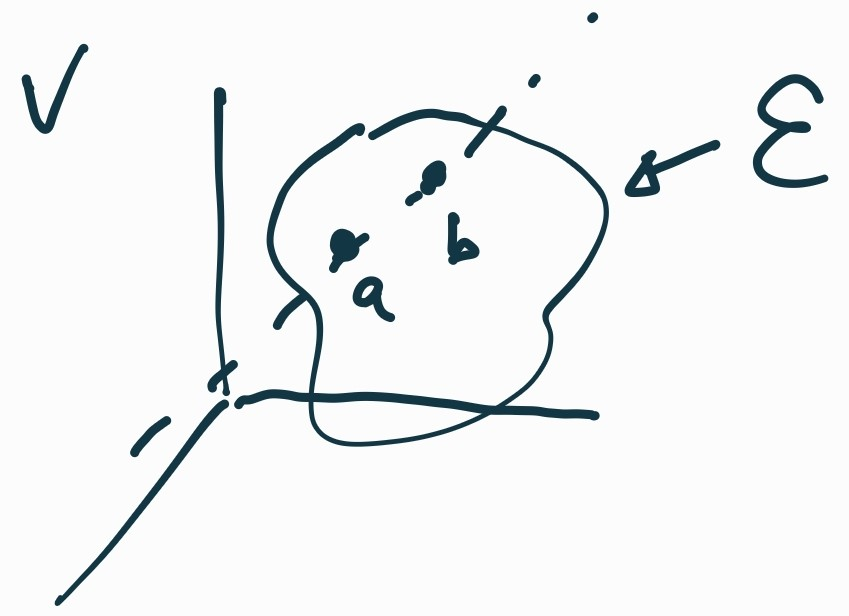
\includegraphics[width=0.4\textwidth]{tempimages/BoundedEnsembleSpace.jpg}
	\caption{$\Ens$ is the ensemble space and $V$ is the embedding vector space. Taking two ensembles, the dashed line represents all the affine combinations. Those that are in the ensemble space are a line, as defined below.}
\end{figure}

\begin{mathSection}
\begin{defn}
	A \textbf{line} $A \subseteq \Ens$ is a convex subset such that for any three elements one can be expressed as a mixture of the other two. That is, for all $\ens_1, \ens_2, \ens_3 \in A$ there exists a permutation $\sigma : \{1,2,3\} \to \{1,2,3\}$ and $p \in [0,1]$ such that $\ens_{\sigma(1)} = p \ens_{\sigma(2)} + \bar{p} \ens_{\sigma(3)}$.
\end{defn}

\begin{prop}
	Given $\ens[a], \ens[b] \in \Ens$, there is only one line that contains them.
\end{prop}

\begin{proof}
	Since an ensemble space embeds into a vector space, given two ensembles there is only one affine line that connects them. A line is the intersection of the affine line with the ensemble space.
\end{proof}

\begin{thrm}[Lines are bounded]
	Let $A \subseteq \Ens$ be a line. Then we can find a bounded interval $V \subseteq \mathbb{R}$ and an invertible function $f : A \to V$ such that $f(p \ens[a] + \bar{p} \ens[b]) = p f(\ens[a]) + \bar{p} f(\ens[b])$ for all $\ens[a], \ens[b] \in A$.
\end{thrm}

\begin{proof}
	Let $A \subseteq \Ens$ be a line. Pick $\ens_0, \ens_1 \in A$. For any $\ens[a] \in A$, we can find an affine expression between $\ens_0$, $\ens_1$ and $\ens[a]$. Rearranging the terms, we can always write $\ens[a] = \bar{x}\ens_0 + x\ens_1$ where $x \in \mathbb{R}$. Note that $x$ uniquely determines $\ens[a]$. Therefore we can define $f(\ens[a]) \mapsto x$, and it will be an invertible function.
	
	We can verify that, given $\ens[a], \ens[b] \in A$, we have
	\begin{equation}
		\begin{aligned}
			f(p\ens[a] + \bar{p} \ens[b]) &= f(p\bar{x}_a \ens_0 + px_a \ens_1 + \bar{p}\bar{x}_b \ens_0 + \bar{p}x_b \ens_1) = f((p\bar{x}_a + \bar{p}\bar{x}_b) \ens_0 + (px_a + \bar{p}x_b) \ens_1) \\
			&= px_a + \bar{p}x_b = pf(\ens[a]) + \bar{p}f(\ens[b]).
		\end{aligned}
	\end{equation}
	
	We are going to show that the image $V=f(A)$ must be a bounded set, or it would eventually violate the entropy bounds. Given a value $x \in V$, there will be an entropy value $S(f^{-1}(x))$ which we can write as a function of the real value $S(x)$. This function will need to satisfy continuity, strict concavity and the upper variability bound.

\begin{figure}[H]
	\centering
	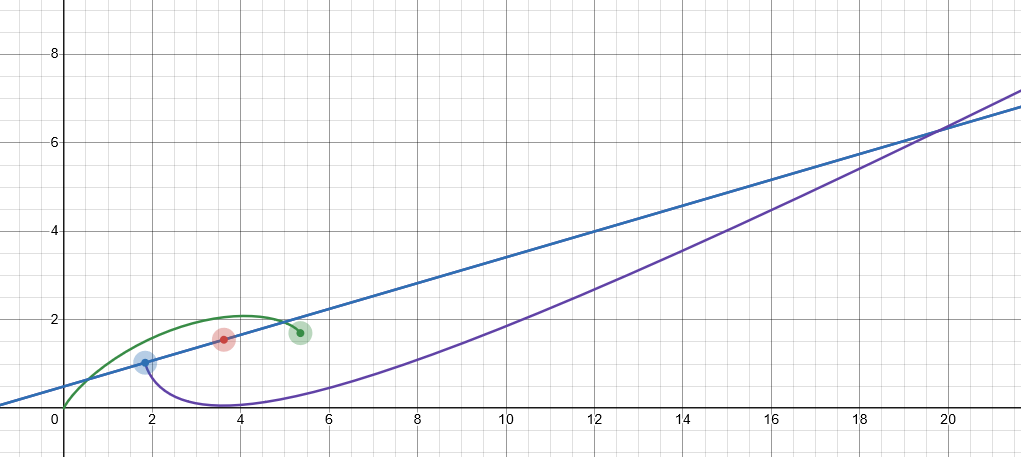
\includegraphics[width=0.7\textwidth]{tempimages/BoundsFromEntropy.png}
	\caption{Visual representation of the bounds. See proof for details.}
\end{figure}
	We are going to show that the function $S(x)$ cannot extend to plus infinity. The same argument can be applied by symmetry for minus infinity. We are going to assume that $S(0) = 0$ without loss of generality. If $S$ is not defined at zero, or if the value is different, we can apply a translation on the argument or on the value, which will not affect the concavity of the function.
	
	Let $0 < a < b \in V$ be two distinct values, with $S(a)$ and $S(b)$ their respective entropies. We are going to show that if we pick a $c > b$ sufficiently large, we are not going to find a value for $S(c)$ that satisfies the bounds. In the picture, we have the three points, $a$ in blue, $b$ in red, $c$ in green. The horizontal axis represent the value, the position of the ensemble along the affine line, while the vertical axis represents the entropy. Consider the points $a$, $b$ and $c$. Since the entropy is strictly concave, $c$ must be placed under the blue line which represents an upper bound on $S(c)$. Now consider $0$, $a$ and $c$. Since $a$ is a mixture of $0$ and $c$, $S(a)$ will need to satisfy the upper bound given by $S(0)$ and $S(c)$. In the diagram, the green line represents the upper bound on $S(a)$ for the specific choice of $c$ and $S(c)$. Since $a$ and $S(a)$ are fixed, this puts a lower bound on $S(c)$, which is represented by the purple curve. That is, the purple curve represents the minimum value we have to assign to $S(c)$ such that $S(a)$ still satisfies the upper bound between $0$ and $c$. As the picture shows, the two bounds meet at some point and cannot both be satisfied.
	
	From strict concavity, noting that $\frac{c-b}{c-a} + \frac{b-a}{c-a} = 1$, we have:
	\begin{equation}
		\begin{aligned}
			S(b) &= S\left(\frac{c-b}{c-a} a + \frac{b-a}{c-a} c\right) > \frac{c-b}{c-a} S(a) + \frac{b-a}{c-a} S(c)\\
			(b-a)S(c) &< (c-a) S(b) - (c-b) S(a) = (c-a) S(b) - (c-a) S(a) + (b-a) S(a) \\
			S(c) &< \frac{S(b) - S(a)}{(b-a)} (c-a) + S(a) \\
		\end{aligned}
	\end{equation}
	
	From the upper bound, noting that $\frac{c-a}{c} + \frac{a}{c} = 1$ and recalling we assumed $S(0) = 0$, we have:
	\begin{equation}
		\begin{aligned}
			S(a) &= S\left(\frac{c-a}{c} 0 + \frac{a}{c} c\right) \leq I\left(\frac{c-a}{c}, \frac{a}{c}\right) + \frac{c-a}{c} S(0) +\frac{a}{c} S(c) \\
			\frac{a}{c} S(c) &\geq S(a) - I\left(\frac{c-a}{c}, \frac{a}{c}\right) \\
			S(c) &\geq \frac{c}{a} \left[ S(a) - I\left(\frac{c-a}{c}, \frac{a}{c}\right) \right]
		\end{aligned}
	\end{equation}
	
	Combining the bounds, we have:
	\begin{equation}
		\begin{aligned}
			\frac{S(b) - S(a)}{(b-a)} (c-a) + S(a) &> \frac{c}{a} \left[ S(a) - I\left(\frac{c-a}{c}, \frac{a}{c}\right) \right] \\
			(c-a) S(b) - (c-a)S(a) + (b-a) S(a) &> \frac{c(b-a)}{a} S(a) - \frac{c(b-a)}{a} I\left(\frac{c-a}{c}, \frac{a}{c}\right) \\
			a (c-a) S(b) - a(c-b) S(a) &> c(b-a)S(a) - c(b-a) I\left(\frac{c-a}{c}, \frac{a}{c}\right) \\
			a (c-a) S(b) + (-ac +ab -bc +ac) S(a) &> - c(b-a) I\left(\frac{c-a}{c}, \frac{a}{c}\right) \\
			a (c-a) S(b) -b (c-a) S(a) &> - c(b-a) I\left(\frac{c-a}{c}, \frac{a}{c}\right) \\
			a  S(b) - b S(a) &> - \frac{c(b-a)}{(c-a)} I\left(\frac{c-a}{c}, \frac{a}{c}\right) \\
		\end{aligned}
	\end{equation}
	
	Since $b > a$, $c > a$ and $I(p,\bar{p}) > 0$ for all $p \in (0,1)$, the right hand side of the inequality is always negative. As $c$ increases, the right hand side will go to zero, since $\lim\limits_{c\to \infty}\frac{c(b-a)}{c-a} = b-a$ and $\lim\limits_{c\to \infty} I\left(\frac{c-a}{c}, \frac{a}{c}\right) = I(1,0) = 0$. The left hand side is a constant. If the constant is positive, the inequality is always satisfied. If it is negative, it will not be satisfied for all $c$.
	
	From strict concavity, noting that $\frac{b-a}{b} + \frac{a}{b} = 1$, we have
	\begin{equation}
		\begin{aligned}
			S(a) &= S\left(\frac{b-a}{b} 0 + \frac{a}{b} b\right) > \frac{b-a}{b} S(0) + \frac{a}{b} S(b) = \frac{a}{b} S(b)\\
			b S(a) &> a S(b)  \\
			0 &> a S(b) - b S(a)\\
		\end{aligned}
	\end{equation}
	This shows that the left hand side of the previous inequality is negative, and therefore the bounds cannot be satisfied over the whole $\mathbb{R}$.
	
	This means that $V = f(A)$ must be bounded and therefore every line is a segment as embedded in the vector space.
\end{proof}

\begin{remark}
	Note that this does not mean that, along each direction, the line is closed in the vector space. That is, it may not include the extreme points. in the convex space. An open bounded interval, in fact, is still a convex space and we would be able to define an entropy on it.
\end{remark}
\end{mathSection}

\section{Entropic geometry}

We now show that the entropy imposes a geometric structure on the ensemble space. The core idea is that, since the entropy is strictly concave, its Hessian is negative definite. The negation is therefore a positive definite, real-valued function of two variations and plays the role of a metric tensor.

\subsection{Mixing entropy as pseudo-distance}

The first observation is that the entropy can be used to define a pseudo-distance. If we mix two ensembles, in fact, the average entropy cannot decrease, and will stay the same if the two components of the mixture are the same ensemble. The increase, then, is zero if the two ensembles are equal, greater than zero if not, with the maximum if they are orthogonal. 

\begin{mathSection}
\begin{defn}
	Given two ensembles $\ens[a], \ens[b] \in \Ens$, the \textbf{mixing entropy}, also called Jensen-Shannon divergence, is the increase in entropy associated to their equal mixture. That is:
	$$MS(\ens[a], \ens[b]) = S\left(\frac{1}{2}\ens[a] + \frac{1}{2} \ens[b]\right) - \left(\frac{1}{2} S(\ens[a]) + \frac{1}{2} S(\ens[b])\right).$$
\end{defn}

\begin{prop}
	The mixing entropy $MS(\ens[a], \ens[b])$ satisfies the following:
	\begin{enumerate}
		\item \textbf{non-negativity}: $MS(\ens[a], \ens[b]) \geq 0$
		\item \textbf{identity of indiscernibles}: $MS(\ens[a], \ens[b]) = 0 \iff \ens[a]=\ens[b]$
		\item \textbf{unit boundedness}: $MS(\ens[a], \ens[b]) \leq 1$
		\item \textbf{maximality of orthogonals}: $MS(\ens[a], \ens[b]) = 1 \iff \ens[a] \ortho \ens[b]$
		\item \textbf{symmetry}: $MS(\ens[a], \ens[b]) = MS(\ens[b], \ens[a])$
	\end{enumerate}
\end{prop}

\begin{proof}
	For 1, by strict concavity, $S\left(\frac{1}{2} \ens[a] + \frac{1}{2} \ens[b]\right) \geq \frac{1}{2} S(\ens[a]) + \frac{1}{2} S(\ens[b])$, which means $S\left(\frac{1}{2} \ens[a] + \frac{1}{2} \ens[b]\right) - \left(\frac{1}{2} S(\ens[a]) + \frac{1}{2} S(\ens[b])\right) = MS(\ens[a], \ens[b]) \geq 0$.
	
	For 2, the concavity is strict and therefore the equality holds if and only if $\ens[a] = \ens[b]$.
	
	For 3, by the upper variability bound, $S\left(\frac{1}{2} \ens[a] + \frac{1}{2} \ens[b]\right) \leq I(\frac{1}{2}, \frac{1}{2}) + \frac{1}{2} S(\ens[a]) + \frac{1}{2} S(\ens[b])$, which means $S\left(\frac{1}{2} \ens[a] + \frac{1}{2} \ens[b]\right) - \left(\frac{1}{2} S(\ens[a]) + \frac{1}{2} S(\ens[b])\right) = MS(\ens[a], \ens[b]) \leq I(\frac{1}{2}, \frac{1}{2}) = 1$.
	
	For 4, the upper variability bound is saturated if and only if $\ens[a] \ortho \ens[b]$.
	
	For 5, by commutativity of mixing and of addition the definition of the mixing entropy is symmetric.
\end{proof}

\begin{prop}
	In discrete and continuous classical cases, the mixing entropy coincides with the Jensen-Shannon divergence. In quantum spaces it coincindes with the quantum Jensen-Shannon divergence.
\end{prop}

\begin{proof}
	Looking at the definitions of the \href{https://en.wikipedia.org/wiki/Jensen%E2%80%93Shannon_divergence}{Jensen-Shannon divergence}, one can see that
	$$ JSD(\ens[a], \ens[b]) = S\left(\frac{1}{2}\ens[a] + \frac{1}{2}\ens[b] \right)  - \frac{1}{2} \left(S(\ens[a]) + S(\ens[b])\right) = MS(\ens[a], \ens[b]).$$
	The same is true for the quantum case:
	$$ QJSD(\ens[a], \ens[b]) = S\left(\frac{1}{2}\ens[a] + \frac{1}{2}\ens[b] \right)  - \frac{1}{2} \left(S(\ens[a]) + S(\ens[b])\right) = MS(\ens[a], \ens[b]).$$
\end{proof}

\begin{remark}
	The mixing entropy fails to be a distance function as it does not satisfy the triangle inequality. In the classical and quantum case, in fact, the JSD and QJSD are the square of a distance function. It is unclear whether this result can be generalized to the mixing entropy itself.
	
	The lack of the triangle inequality also makes it difficult to show that the topology is Hausdorff. The mixing entropy, in fact, allows us to create open balls around each point. These open balls will shrink to each point as the radius goes to zero. However, one typically uses the triangle inequality to show that the open balls, at some point, become disjoint.
\end{remark}
\end{mathSection}

\subsection{Entropic metric}

The second observation is that the strict concavity of the entropy forces the Hessian to be negative definite. The negation of the Hessian, then, is a positive definite function of two variations. In general, the Hessian of a scalar function is not a tensor. However, the ensemble space is a linear space and that linearity has physical significance. It is only for coordinates linear with respect to the mixing coefficient that the convex combination of coordinates will equal the statistical mixture of the corresponding ensembles. Therefore the metric tensor corresponds to the Hessian calculated on that linear structure. When using non-linear coordinates, as long as the coordinates are smooth, one can always make the appropriate transformation to linear coordinates.

\begin{mathSection}
\begin{remark}
	In this section we will assume that an ensemble space embeds continuously into a topological vector space, even though we have not yet proved it. We are going to talk about variations $\delta \ens$ on the space, even though it is not yet clear exactly which mathematical approach is best to make variations well-defined. We are also going to talk about a metric tensor even though the space is not, in general, a manifold.
\end{remark}
	
\begin{defn}
	An ensemble space is \textbf{smooth} if the entropy is twice differentiable with respect to the mixing coefficients.
\end{defn}

\begin{prop}
	Discrete and continuous classical ensemble spaces and quantum ensemble spaces are smooth.
\end{prop}

\begin{proof}
	In both the discrete classical case and the quantum case the entropy of an ensemble is the Shannon entropy of a decomposition in terms of pure states. The Shannon entropy is a smooth function of the coefficients. For the continuous classical case, the differential entropy is a smooth function of the probability density, which is linear under mixture. Therefore the entropy is always smooth with respect to mixing coefficients.
\end{proof}

\begin{defn}
	Assuming $\Ens$ embeds in a topological vector space, given $\ens \in \Ens$ a \textbf{variation} $\delta \ens$ of $\ens$ is a vector in the ambient space such that $\forall t \in [0,1]$ $\ens + t \delta \ens \in \Ens$. Unless otherwise noted, we assume the variation is expressed on the affine structure. Note that it can be re-expressed through a non-linear map as long as the map is differentiable (i.e. it maps variations to variations).
\end{defn}

\begin{remark}
	Note that since an ensemble space is a convex subset of a real vector space, coordinate systems that are linear with respect to the vector space are privileged. It is only in these coordinates, in fact, that linear combinations correspond to mixtures. The strict concavity of the entropy is therefore guaranteed in these coordinates and only these coordinates. Given the special physical significance of these coordinates, all differential objects and properties will be defined in these coordinates.
\end{remark}

\begin{defn}
	Given an ensemble $\ens \subseteq \Ens$ and a variation $\delta \ens$ defined at that point, the \textbf{norm} of $\delta \ens$ is given by
	$$ \lVert \delta \ens \rVert_{\ens} = \sqrt{ 8 MS(\ens, \ens + \delta \ens) }.$$
	The \textbf{metric tensor} (i.e. the inner product between $\delta \ens_1 , \delta \ens_2 \in T_{\ens}$) is given by
	$$ g_{\ens}( \delta \ens_1, \delta \ens_2 ) = \frac{1}{2} \left( \lVert \delta \ens_1 + \delta \ens_2 \rVert_{\ens}^2 - \lVert \delta \ens_1 \rVert_{\ens}^2 - \lVert \delta \ens_2 \rVert_{\ens}^2 \right).$$
\end{defn}

\begin{thrm}
	Let $\Ens$ be a smooth ensemble space. Then, on the affine structure, we have
	$$ \lVert \delta \ens \rVert_{\ens}^2 = - \frac{\partial^2 S}{\partial \ens^2}(\delta \ens , \delta \ens) $$
	and 
	$$ g_{\ens}( \delta \ens_1, \delta \ens_2 ) = - \frac{\partial^2 S}{\partial \ens ^2}( \delta \ens_1, \delta \ens_2 ).$$
\end{thrm}

\begin{proof}
	To recover the first two expressions, we simply have to calculate the leading term. Since the entropy is twice differentiable, on the affine structure, we can expand it as
	\begin{equation}
		\begin{aligned}
			S(\ens + \delta \ens) &= S(\ens) + \frac{\partial S}{\partial \ens} \delta \ens + \frac{1}{2} \frac{\partial^2 S}{\partial \ens^2} \delta \ens \delta \ens + O(\delta \ens ^3).
		\end{aligned}
	\end{equation}
	Expanding the definition of $MS$, we have
	\begin{equation}
		\begin{aligned}
			MS(\ens, \ens + \delta \ens) &= S\left(\frac{1}{2} \ens + \frac{1}{2}(\ens + \delta \ens) \right) - \frac{1}{2} S(\ens) - \frac{1}{2} S(\ens+\delta \ens) \\
			&=  S\left(\ens + \frac{1}{2} \delta \ens \right) - \frac{1}{2} S(\ens) - \frac{1}{2} S(\ens+\delta \ens) \\
			&= S(\ens) + \frac{\partial S}{\partial \ens} \frac{1}{2}\delta \ens + \frac{1}{2} \frac{\partial^2 S}{\partial \ens^2} \frac{1}{2}\delta \ens \frac{1}{2}\delta \ens + O(\delta \ens ^3) \\
			&- \frac{1}{2} S(\ens) - \frac{1}{2} \left( S(\ens) + \frac{\partial S}{\partial \ens} \delta \ens + \frac{1}{2} \frac{\partial^2 S}{\partial \ens^2} \delta \ens \delta \ens + O(\delta \ens ^3) \right) \\
			&= S(\ens) + \frac{1}{2} \frac{\partial S}{\partial \ens} \delta \ens + \frac{1}{8} \frac{\partial^2 S}{\partial \ens^2} \delta \ens \delta \ens \\
			&- S(\ens) - \frac{1}{2} \frac{\partial S}{\partial \ens} \delta \ens - \frac{1}{4} \frac{\partial^2 S}{\partial \ens^2} \delta \ens \delta \ens + O(\delta \ens ^3) \\
			&= - \frac{1}{8} \frac{\partial^2 S}{\partial \ens^2} \delta \ens \delta \ens + O(\delta \ens ^3).
		\end{aligned}
	\end{equation}
	
	Therefore
	$$ \lVert \delta \ens \rVert^2 = 8 MS(\ens, \ens + \delta \ens) = -  \frac{\partial^2 S}{\partial \ens^2} (\delta \ens, \delta \ens).$$
	
	We can now substitute the norm in the definition of the metric tensor. We have
	\begin{equation}
		\begin{aligned}
			g_{\ens}(\delta \ens_1, \delta \ens_2 ) &= \frac{1}{2} \left( \lVert \delta \ens_1 + \delta \ens_2 \rVert^2 - \lVert \delta \ens_1 \rVert^2 - \lVert \delta \ens_2 \rVert^2 \right) \\
			&= \frac{1}{2} \left( - \frac{\partial^2 S}{\partial \ens^2} (\delta \ens_1 + \delta \ens_2, \delta \ens_1 + \delta \ens_2) + \frac{\partial^2 S}{\partial \ens^2} (\delta \ens_1, \delta \ens_1) + \frac{\partial^2 S}{\partial \ens^2} (\delta \ens_2, \delta \ens_2) \right) \\
			&= - \frac{1}{2} \left(  \frac{\partial^2 S}{\partial \ens^2} (\delta \ens_1, \delta \ens_1) + \frac{\partial^2 S}{\partial \ens^2} (\delta \ens_1, \delta \ens_2) + \frac{\partial^2 S}{\partial \ens^2} (\delta \ens_2, \delta \ens_1) + \frac{\partial^2 S}{\partial \ens^2} (\delta \ens_2, \delta \ens_2) \right. \\
			&-  \left. \frac{\partial^2 S}{\partial \ens^2} (\delta \ens_1, \delta \ens_1) - \frac{\partial^2 S}{\partial \ens^2} (\delta \ens_2, \delta \ens_2) \right) \\
			&= - \frac{\partial^2 S}{\partial \ens^2} (\delta \ens_1, \delta \ens_2). \\
		\end{aligned}
	\end{equation}
\end{proof}
\end{mathSection}

We now show that the metric tensor we defined reduces to the Fisher-Rao metric in the classical case and to its quantum equivalent in the quantum case.

\begin{mathSection}
\begin{prop}
	For a continuous classical ensemble space, the metric corresponds to the Fisher-Rao metric.
\end{prop}

\begin{proof}
	Let $\Ens$ be a continuous classical ensemble space. Each ensemble is a classical probability density $\rho$. Let $V \subseteq \Ens$ be a manifold of probability distributions over $X$ parametrized by $\theta^i$. The \href{https://en.wikipedia.org/wiki/Fisher_information_metric}{Fisher-Rao metric} is defined as:
	\begin{equation}
		g_{ij} =- \int_X \frac{\partial^2 \log \rho}{\partial \theta^i \partial \theta^j} \rho dx.
	\end{equation}
	where $\log$ will be the natural logarithm throughout this calculation. Recall that for a continuous classical ensemble, the entropy is given by
	\begin{equation}
		S(\rho) =- \int_X \rho \log \rho dx.
	\end{equation}
	
	Let us now calculate the first two terms in the Taylor expansion around $\rho$ with a variation $\delta\rho$. Recall that
	\begin{equation}
		\begin{aligned}
			\log(x+dx) &= \log(x) + d_x \log x \, dx + \frac{1}{2} d_x d_x  \log x \, dx^2 + O(dx^3) \\
			&= \log(x) + \frac{1}{x} dx - \frac{1}{2} \frac{1}{x^2} dx^2 + O(dx^3).
		\end{aligned}
	\end{equation}
	We have
	\begin{equation}
		\begin{aligned}
			S(\rho + \delta \rho) &= -\int_X (\rho + \delta \rho) \log (\rho + \delta \rho) dx \\
			&=-\int_X (\rho + \delta \rho) \left[\log \rho + \frac{1}{\rho} \delta \rho - \frac{1}{2\rho^2} \delta \rho^2 + O(\delta \rho^3)\right] dx \\
			&= - \int_X \rho \log \rho dx - \int_X \left[\log \rho + 1 \right]dx \delta \rho -\int_X \left[\frac{1}{\rho} - \frac{\rho}{2\rho^2}\right] dx \delta \rho^2 + \int_X dx O(\delta\rho^3) \\
			&= - \int_X \rho \log \rho dx - \int_X \left[\log \rho + 1 \right]dx \delta \rho - 	
			\frac{1}{2}\int_X \frac{1}{\rho} dx \delta \rho^2 + \int_X dx O(\delta\rho^3) \\
		\end{aligned}
	\end{equation}
	\begin{equation}
		\begin{aligned}
			\frac{\partial^2 S}{\partial \rho^2}(\delta \rho, \delta \rho) &= -\int_X \frac{1}{\rho} \delta \rho^2 dx = -\int_X \frac{1}{\rho} \delta \rho^2 dx + 0 = -\int_X \frac{1}{\rho} \delta \rho^2 dx + \delta^2 (1) \\
			&= -\int_X \frac{1}{\rho} \delta \rho^2 dx + \delta^2 \int_X \rho dx = -\int_X \frac{1}{\rho} \delta \rho^2 dx + \int_X \delta^2 \rho dx \\
			&= \int_X \rho dx \left[-\frac{1}{\rho^2} \delta \rho^2 + \frac{1}{\rho} \delta^2 \rho \right]
			= \int_X \rho dx \, \delta \left[\frac{1}{\rho} \delta \rho \right] \\
			&= \int_X \rho dx \, \delta^2 \log \rho.
		\end{aligned}
	\end{equation}
	
	Let us consider a family of ensembles charted by a set of parameters $\theta^i$, not necessarily forming a linear chart. We have
	\begin{equation}
		\begin{aligned}
			g_{\ens}(d\theta^i, d\theta^j) &= - \frac{\partial^2 S}{\partial \rho^2}\left(\frac{\partial 
				\rho}{\partial \theta^i} d\theta^i, \frac{\partial 
				\rho}{\partial \theta^j} d\theta^j\right) = - \int_X \rho dx \frac{\partial^2 \log \rho}{\partial \theta^i \partial \theta^j}d\theta^i d\theta^j
		\end{aligned}
	\end{equation}
	which recovers the Fisher-Rao metric.
\end{proof}

TODO: add a note/proof for the discrete version

\begin{remark}
	For quantum mechanics, the situation is more complicated as there are different definitions of Fisher metrics (see \href{https://arxiv.org/pdf/2008.11178}{RLD Fisher Information Bound for Multiparameter
		Estimation of Quantum Channels} or \href{https://link.springer.com/chapter/10.1007/978-4-431-54493-7_4}{Quantum Estimation Theory}). We will therefore just show a general connection, without worrying about the mathematical details.
	
\end{remark}

\begin{prop}
	For a quantum ensemble space, the metric corresponds to the Bures metric and the Quantum Fisher information metric.
\end{prop}

\begin{proof}
	Since we are working in a quantum ensemble space, each ensemble is a density operator $\rho$. The entropy is given by the von Neumann entropy
	\begin{equation}
		S(\rho) = - \tr\left(\rho \log \rho\right).
	\end{equation}
	We take the first variation and have
	\begin{equation}
		\begin{aligned}
			\delta S(\rho) &= - \delta \tr\left(\rho \log \rho\right)= - \tr\left(\delta \rho \log \rho + \rho \delta \log \rho\right) \\
			&= - \tr\left(\delta \rho \log \rho + \rho \rho^{-1} \delta \rho \right) \\
			&= - \tr\left(\left(\log \rho + 1 \right) \delta \rho \right).
		\end{aligned}
	\end{equation}
	We take the second variation and have
	\begin{equation}
		\begin{aligned}
			\delta^2 S(\rho) &= - \delta \tr\left(\left(\log \rho + 1 \right) \delta \rho \right) \\
			&= - \tr\left(\delta \left(\log \rho + 1 \right) \delta \rho + \left(\log \rho + 1 \right) \delta \delta \rho \right) \\
			&= - \tr\left(\rho^{-1} \delta \rho \delta \rho + \left(\log \rho + 1 \right) \delta \delta \rho \right).
		\end{aligned}
	\end{equation}
	Note that $\delta \rho$ is defined in a linear chart, therefore $\delta \delta \rho = 0$. Therefore we have 
	\begin{equation}
		\begin{aligned}
			\frac{\partial^2 S}{\partial \rho^2}(\delta \rho, \delta \rho) &= - \tr\left(\rho^{-1} \delta \rho \delta \rho \right).
		\end{aligned}
	\end{equation}
	Let us consider a family of ensembles charted by a set of parameters $\theta^i$, not necessarily forming a linear chart. We have
	\begin{equation}
		\begin{aligned}
			g_{\ens}(d\theta^i, d\theta^j) &= - \frac{\partial^2 S}{\partial \rho^2}\left(\frac{\partial 
				\rho}{\partial \theta^i} d\theta^i, \frac{\partial 
				\rho}{\partial \theta^j} d\theta^j\right) = \tr\left( \rho^{-1} \frac{\partial \rho}{\partial \theta^i }\frac{\partial \rho}{\partial \theta^j}\right) d\theta^i d\theta^j
		\end{aligned}
	\end{equation}
	which recovers one version of the Fisher-Rao metric.
	
	Recalling that the right logarithmic derivative (RLD) $L^R$ satisfies $\frac{\partial \rho}{\partial \theta} = \rho L^R$, we can write 
	\begin{equation}
		\begin{aligned}
			g_{\ens}(d\theta^i, d\theta^j) &= \tr\left( \rho^{-1} \frac{\partial \rho}{\partial \theta^i }\frac{\partial \rho}{\partial \theta^j}\right) d\theta^i d\theta^j = \tr(\rho^{-1}\rho L^R
			_i \rho L^R_j)d\theta^i d\theta^j = \tr(\rho L^R
			_i L^R_j)d\theta^i d\theta^j
		\end{aligned}
	\end{equation}
	which recovers the RLD Fisher information.
\end{proof}

\begin{remark}
	Note that these results relate also to the \href{https://en.wikipedia.org/wiki/Ruppeiner_geometry}{Ruppeiner metric}, which is the Hessian of the entropy. They also relate to the Hessian metric as described in  \href{https://web.osu.cz/~Zusmanovich/seminar/2017/wolak/ostrava-11-17-hessian-pdf.pdf}{Hessian structures} \href{https://link.springer.com/chapter/10.1007/978-3-642-40020-9_4}{1}.
\end{remark}
\end{mathSection}

\section{State capacity}

In this section we are going to develop a generalization of the link between count of states and entropy. In classical mechanics, for a uniform distribution $\rho_U$ over a region of phase space $U$, we have $S(\rho_U) = \log \mu(U)$, where $\mu$ is the Liouville measure that is taken to correspond to the count of states. The idea is to generalize this relationship to all ensembles, classical and quantum.

Given an ensemble, we want to quantify the number of distinguishable cases over which the ensemble is spread. Since entropy characterizes the variability of the preparations of the ensemble, greater variability means the ensemble is spread over more cases. Therefore the count of distinguishable states must be a monotonic function of the entropy. The question is what function.

The first hint that the exponential is the right function is the relationship $S(\rho_U) = \log \mu(U)$ mentioned before. Another hint is that we will want this size to be multiplicative over independent distributions. That is, if we have two ensembles $\rho_1 \in \Ens_1$ and $\rho_2 \in \Ens_2$ of two different ensemble spaces, we can imagine the composite system $\rho = \rho_1 \rho_2$ representing the ensemble of the two independent ensembles. While the entropy should be additive, that is $S(\rho) = S_1(\rho_1) + S_2(\rho_2)$, the count of states should be multiplicative, that is $\mu(\rho) = \mu_1(\rho_1) \mu_2(\rho_2)$. This suggests the relationship $S(\rho) = \log \mu (\rho)$ for all ensembles. The other hint is that the spread can be, at most, additive. If we mix two ensembles, the spread can be at most over the configurations of both and not more. The following shows that the exponential of the entropy has exactly that property

\begin{mathSection}
\begin{prop}[Exponential entropy subadditivity]\label{pm_es_exponentialEntropySubadditivity}
	Let $\ens[a], \ens[b] \in \Ens$ and $\ens = p \ens[a] + \bar{p} \ens[b]$ for some $p \in [0,1]$. Then $2^{S(\ens)} \leq 2^{S(\ens[a])} + 2^{S(\ens[b])}$, with the equality holding if and only if $\ens[a] \ortho \ens[b]$ and $p = \frac{2^{S(\ens[a])}}{2^{S(\ens[a])} + 2^{S(\ens[b])}}$.
\end{prop}

\begin{proof}
	If $p$ is fixed, the upper variability bound of entropy is saturated only if $\ens[a]$ and $\ens[b]$ are orthogonal by definition. Therefore the entropy maximum for the mixed ensemble will be achieved when the elements are orthogonal, for some value of $p$.
	
	Now fix the entropy of $\ens[a]$ and $\ens[b]$ to some values $S_a = S(\ens[a])$ and $S_b = S(\ens[b])$. The entropy of the mixture depends only on $p$, so we need to find the $p$ that maximizes the expression. Since $\ens[a]$ and $\ens[b]$ are orthogonal, $S(p \ens[a] + \bar{p}\ens[b]) =  - p \log p - \bar{p} \log \bar{p} + p S_a + \bar{p} S_b$ which is a smooth function of $p$.
	\begin{equation}
		\begin{aligned}
			0 &= \frac{d}{dp} S(p \ens[a] + \bar{p}\ens[b]) =\frac{d}{dp} \left( - p \log p - \bar{p} \log \bar{p} + p S_a + \bar{p} S_b \right) \\
			&= - \log p - 1 + \log \bar{p} + 1 + S_a - S_b \\
			\log \frac{p}{\bar{p}} &= \log 2^{S_a} - \log 2^{S_b} \\
			\log \frac{p}{1-p} &= \log \frac{2^{S_a}}{2^{S_b}}  \\
			p 2^{S_b} &= (1-p) 2^{S_a}  \\
			p (2^{S_a} + 2^{S_b}) &= 2^{S_a}  \\
			p &= \frac{2^{S_a}}{2^{S_a} + 2^{S_b}}  \\
		\end{aligned}
	\end{equation}
	Having found the value of $p$ that maximizes the entropy, we can calculate the maximum entropy.
	\begin{equation}
		\begin{aligned}
			\bar{p} &= 1- \frac{2^{S_a}}{2^{S_a} + 2^{S_b}} = \frac{2^{S_b}}{2^{S_a} + 2^{S_b}} \\
			S(p \ens[a] + \bar{p}\ens[b]) &= - p \log p - \bar{p} \log \bar{p} + p S_a + \bar{p} S_b  \\
			&= - \frac{2^{S_a}}{2^{S_a} + 2^{S_b}} \log \frac{2^{S_a}}{2^{S_a} + 2^{S_b}} - \frac{2^{S_b}}{2^{S_a} + 2^{S_b}} \log \frac{2^{S_b}}{2^{S_a} + 2^{S_b}} \\
			&+ \frac{2^{S_a}}{2^{S_a} + 2^{S_b}} \log 2^{S_a} + \frac{2^{S_b}}{2^{S_a} + 2^{S_b}} \log 2^{S_b} \\
			&= \frac{2^{S_a}}{2^{S_a} + 2^{S_b}} \log \left( 2^{S_a} + 2^{S_b} \right) + \frac{2^{S_b}}{2^{S_a} + 2^{S_b}} \log \left( 2^{S_a} + 2^{S_b} \right) \\
			&= \frac{2^{S_a} + 2^{S_b}}{2^{S_a} + 2^{S_b}} \log \left( 2^{S_a} + 2^{S_b} \right) \\
			\log 2^{S(p \ens[a] + \bar{p}\ens[b])} &= \log \left( 2^{S_a} + 2^{S_b} \right) \\
			2^{S(p \ens[a] + \bar{p}\ens[b])} &=  2^{S_a} + 2^{S_b}  \\
		\end{aligned}
	\end{equation}
	Therefore the maximum entropy obtainable through a mixture is $S(p \ens[a] + \bar{p}\ens[b]) = \log (2^{S(\ens[a])} + 2^{S(\ens[b])})$ which is obtained when $\ens[a]$ and $\ens[b]$ are orthogonal and $p = \frac{2^{S(\ens[a])}}{2^{S(\ens[a])} + 2^{S(\ens[b])}}$.
\end{proof}

\begin{remark}
	We have proved that the exponential of the entropy gives us subadditivity. Ideally, we should prove that this is the only function with that characteristic.
\end{remark}

\begin{conj}
	Let $f : \mathbb{R} \to \mathbb{R}$ be a continuous function such that $f(S(p\ens[a]+\bar{p}\ens[b])) \leq f(S(\ens[a])) + f(S(\ens[b]))$ and the equality can be verified in some condition. Then $f(x) = \kappa^x$ for some arbitrary constant $\kappa$.
\end{conj}
\end{mathSection}

Given a set of ensembles, we can ask what spread is reachable by a mixture in terms of the number of distinguishable states. We call this the state capacity as it represents the maximum potential spread reachable by the set, and because it turns out to be a non-additive measure.\footnote{In some literature, capacities are non-additive measures.} The state capacity is monotone, subadditive and recovers additivity over orthogonal sets.

\begin{mathSection}
\begin{defn}
	Let $A \subseteq \Ens$ be the subset of an ensemble space. The \textbf{state capacity} of $A$ is defined as $\capacity(A) = \sup(2^{S(\hull(A))}\cup\{0\})$.
\end{defn}

\begin{prop}
	The state capacity is a set function that is
	\begin{enumerate}
		\item non-negative: $\capacity(A) \in [0, +\infty]$
		\item monotone: $A \subseteq B \implies \capacity(A) \leq \capacity(B)$
		\item subadditive: $\capacity(A \cup B) \leq \capacity(A) + \capacity(B)$
		\item additive over orthogonal sets: $A \ortho B \implies \capacity(A \cup B) = \capacity(A) + \capacity(B)$ 
	\end{enumerate}
\end{prop}

\begin{proof}
	1. The state capacity takes a subset of $\Ens$ and returns a real value and is therefore a set function. The exponential can only return non-negative values, therefore the state capacity of a set is non-negative. 
	
	2. The $\hull$ is a monotone function. The image of a set through a map is a monotone function. The supremum is a monotone function. Therefore the state capacity is a monotone function.
	
	3. Let $A, B \subseteq \Ens$ and let $\ens = p \ens[a] + \bar{p} \ens[b]$ for some $p \in [0,1]$, $\ens[a] \in A$ and $\ens[b] \in B$. By \ref{pm_es_exponentialEntropySubadditivity} and the definition of state capacity, $2^{S(\ens)} \leq 2^{S(\ens[a])} + 2^{S(\ens[b])} \leq \capacity(A) + \capacity(B)$. Since this is true for any finite mixture of elements of $A$ and $B$, it will also be true for any element of $\hull(A \cup B)$ since the entropy is continuous. Consequently, the supremum of the exponential entropy cannot exceed the sum of the state capacities. Therefore $\capacity(A \cup B) \leq \capacity(A) + \capacity(B)$ (i.e. the state capacity is subadditive).
	
	4. Let $A, B \subseteq \Ens$ be two orthogonal subsets. Let $\{\ens[a]_i\} \subseteq A$ be a sequence of ensembles such that $2^{S(\ens[a]_i)} \to \capacity(A)$ and let $\{\ens[b]_i\} \subseteq B$ be a sequence of ensembles such that $2^{S(\ens[b]_i)} \to \capacity(B)$. Consider $\ens_i = p_i \ens[a]_i + \bar{p_i} \ens[b]_i$ where $p_i = \frac{2^{S(\ens[a]_i)}}{2^{S(\ens[a]_i)} + 2^{S(\ens[b]_i)}}$. Then, by \ref{pm_es_exponentialEntropySubadditivity}, $2^{S(\ens_i)} = 2^{S(\ens[a]_i)} + 2^{S(\ens[b]_i)}$. This means that $2^{S(\ens_i)} \to \capacity(A) + \capacity(B)$. Therefore $\capacity(A \cup B)$ must be at least $\capacity(A) + \capacity(B)$. Combining with the previous result, $\capacity(A \cup B) = \capacity(A) + \capacity(B)$. Therefore the state capacity, as a set function, is additive over orthogonal sets of ensembles.
\end{proof}

\begin{conj}
	The state capacity is continuous from above and below.
\end{conj}

\begin{conj}
	The state capacity is additive only on orthogonal sets.
\end{conj}

\begin{proof}
	If the state capacity adds, then the states with highest entropy satisfy the upper variability bound and are orthogonal. What needs to be shown is that this is enough to say all elements are orthogonal. There is a series of nice results possible here. If $\ens[a] \ortho \ens[b]$ then $\ens[a]$ is orthogonal to all the components of $\ens[b]$. If $\ens[a]$ is the ensemble with maximum entropy in $\hull(A)$, it should be true that all elements of the hull are components of $\ens[a]$. If one ensemble is not, we should be able to create an ensemble with higher entropy.
\end{proof}
\end{mathSection}

Note that the state capacity for a single element corresponds to the ``ensemble volume'' defined in \href{https://arxiv.org/pdf/physics/9903045}{this work} and more recently \href{https://arxiv.org/pdf/1804.01343}{here}. It is connected to various uncertainty relationships, including a stronger form of the quantum uncertainty principle. It would be interesting to understand what results can be generalized to the ensemble space.

We now show that the state capacity recovers a notion of number of cases in all three target spaces. In the discrete classical case it recovers the number of points; in the continuous classical case, it recovers the Liouville volume; in the quantum case, it recovers the number of orthogonal pure states.

\begin{mathSection}
\begin{prop}
	Let $\Ens$ be a discrete classical ensemble space. Let $U \subseteq \{s_i\}$ be a subset of the corresponding (extreme) points and $A$ be the set of probability distributions whose support is a subset of $U$. Then $\capacity(A) = \#U$.
\end{prop}

\begin{proof}
	Let $A$ be the set of probability distributions defined over a discrete countable set $U$. The highest entropy is achieved by the uniform distribution, which equals $\log (\#U)$. Therefore $\capacity(A) = 2^{\log(\#U)} = \#U$.
\end{proof}

\begin{prop}
	Let $\Ens$ be a continuous classical ensemble space. Let $U \subseteq X$ be a subset of the corresponding symplectic manifold (i.e. phase space) and $A$ be the set of probability distributions whose support is a subset of $U$. Then $\capacity(A) = \mu(U)$ where $\mu(U)$ is the Liouville measure.
\end{prop}

\begin{proof}
	Let $A$ be the set of probability distributions whose support is a subset of $U$. The highest entropy is achieved by the uniform distribution, which equals $\log(\mu(U))$. Therefore $\capacity(A) = 2^{\log(\mu(U))} = \mu(U)$.
\end{proof}

\begin{prop}
	Let $\Ens$ be a quantum ensemble space. Let $U \subseteq \mathcal{H}$ be a subspace of the corresponding Hilbert space and $A$ be the set of density operators defined on that subspace (i.e. zero eigenvalues outside). Then $\capacity(A) = \dim(U)$ where $\dim(U)$ is the dimensionality of the subspace.
\end{prop}

\begin{proof}
	Let $A$ be the set of density operators defined on a subspace $U$. The highest entropy is achieved by the maximally mixed state, which equals $\log(\dim(U))$. Therefore $\capacity(A) = 2^{\log(\dim(U))} = \dim(U)$.
\end{proof}
\end{mathSection}

\section{Fraction capacity and probability}

Having seen how the strict concavity of the entropy leads to geometric structures, we are going to see how mixing is responsible for the measure theoretic structures. In the same way we derived a geometric structure on the ensembles, we are going to first define a measure theoretic structure on the ensembles as well. This measure, the fraction capacity, will tell us how much of an ensemble can be seen as a mixture of a set of others. It is not additive in general, but subadditive.

We are then going to find necessary and sufficient conditions for a subset of ensembles to form a classical probability context, so that each element can be understood as a classical probability measure over a set of cases, over the spectrum of the context. We will see that all classical ensemble spaces are classical probability contexts, while in quantum mechanics the set of mixed states that commutes with a complete set of commuting observables corresponds to a classical probability context.\footnote{In the future we will want to generalize the construction of the spectrum to the whole space.}

\subsection{Fraction and fraction capacity}

%DONE: subsection reviewed by Sharif and Christine

In this section we are going to define \textbf{fraction capacity}, which can be understood as a generalization of probability that works with any ensemble space. The typical way to understand probability is through outcomes of a process: $50\%$ probability for tails means that if we repeated the coin toss multiple times, we would expect roughly half to be tails. In classical mechanics, it can also be understood as the probability of preparation: roughly half the times we selected a preparation procedure that prepared tails. In quantum mechanics, this does not work as the probability used during the mixing is the same as the probability of the outcome only if we are mixing orthogonal states. Effectively, probability in the usual sense is defined only on outcomes. The fraction capacity, instead, defines a measure on preparations.

The fraction capacity tells us how much of an ensemble $\ens$ can be constructed through a mixture of ensembles from a set $A$. It is a non-negative, unit bounded, subadditive, monotone continuous measure, and it reduces to the probability measure in the classical case, and over measurement contexts in the quantum case. The goal is to create a measure theoretic generalization of probability theory that can work on all ensemble spaces.

\begin{figure}[h]
	\centering
	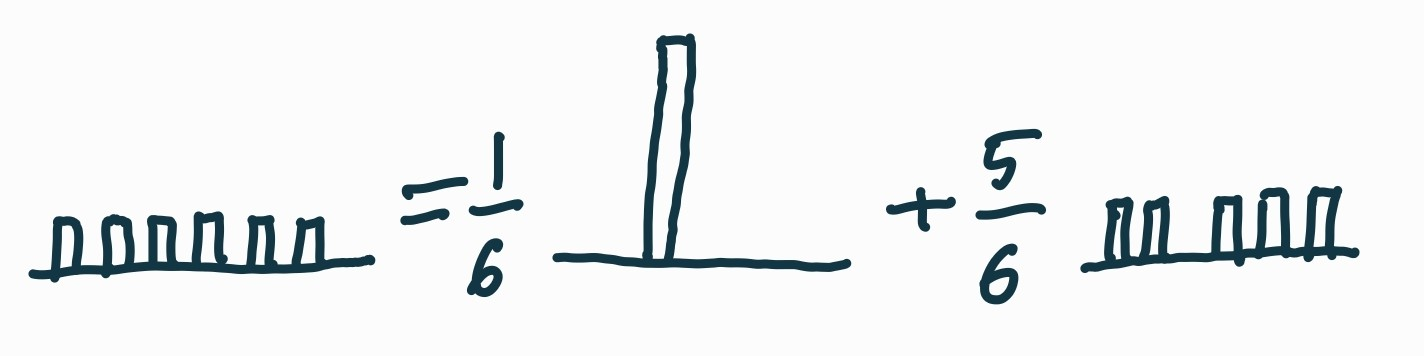
\includegraphics[width=0.6\textwidth]{tempimages/Fraction.jpg}
\end{figure}

First we define the \textbf{fraction} of one element within another. For example, suppose $\ens$ is a uniform distribution for a six-faced die. Suppose $\ens[a]$ represents the outcome 3 with $100\%$ probability. Then $\ens$ can be understood as $\ens = \frac{1}{6} \ens[a] + \frac{5}{6} \ens[b]$ where $\ens[b]$ is the uniform distribution over the outcomes 1,2,4,5 and 6. Note that $\frac{1}{6}$ is the highest coefficient we can put in front of $\ens[a]$ in a convex combination and have $\ens$ as a result, which coincides with the probability of obtaining 3 from a uniform distribution over six outcomes. That is what we define the fraction of $\ens[a]$ in $\ens$ to be.

\begin{mathSection}
	\begin{defn}
		Let $\ens, \ens[a] \in \Ens$ be two ensembles. The \textbf{fraction} of $\ens[a]$ in $\ens$ is the greatest mixing coefficient for which $\ens$ can be expressed as a mixture of $\ens[a]$. That is, $\size_{\ens}(\ens[a]) = \sup(\{ p \in [0,1] \, | \, \exists \, \ens[b] \in \Ens \text{ s.t. }  \ens = p \ens[a] + \bar{p} \ens[b] \})$.
	\end{defn}
\begin{figure}[H]
	\centering
	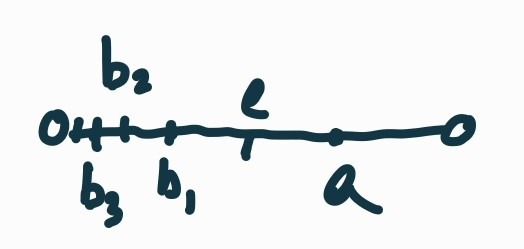
\includegraphics[width=0.4\textwidth]{tempimages/CapacitySupremum.jpg}
\end{figure}
	
	\begin{remark}
		We need to take the supremum as the maximum may not exist. For example, consider a discrete classical ensemble space and remove the extreme points. At the moment, there is no reason to rule out such space as unphysical.
	\end{remark}
	
	\begin{coro}
		Let $\ens, \ens[a] \in \Ens$, then $\size_{\ens}(\ens[a]) = 0$ if and only if $\ens[a]$ is not a component of $\ens$.
	\end{coro}
	
	\begin{proof}
		Note that $\ens[a]$ is a component of $\ens$ if we can write $\ens = \lambda \ens[a] + \bar{\lambda} \ens[b]$ for some $\lambda \in (0,1]$ and $\ens[b] \in \Ens$. In this case, $\size_{\ens}(\ens[a]) \geq \lambda > 0$. Conversely, if $\size_{\ens}(\ens[a]) > 0$ we can find $\size_{\ens}(\ens[a]) \geq \lambda > 0$ such that $\ens = \lambda \ens[a] + \bar{\lambda} \ens[b]$ for some $\ens[b] \in \Ens$.
	\end{proof}
\end{mathSection}

\begin{figure}[h]
	\centering
	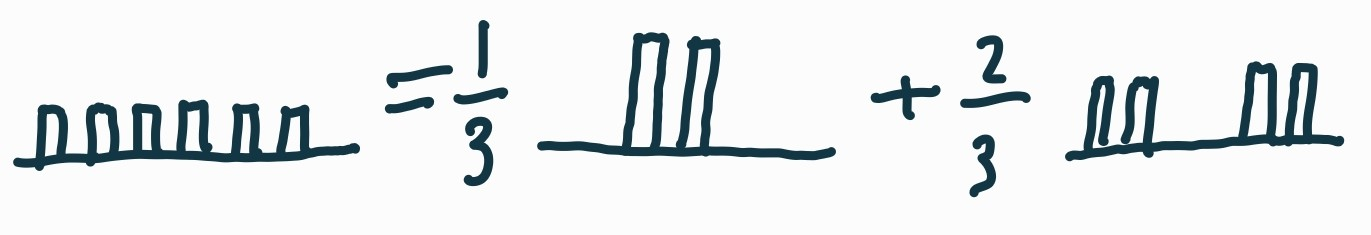
\includegraphics[width=0.6\textwidth]{tempimages/FractionCapacity.jpg}
\end{figure}

We now define \textbf{fraction capacity} of a set of ensembles for another ensemble. Like before, suppose $\ens$ is a uniform distribution for a six-faced die, but now take $A = \{ \ens[a], \ens[b] \}$ as, respectively, the outcomes $3$ and $4$ with $100\%$ probability. Then $\ens$ can be understood as $\ens = \frac{1}{3} \left(\frac{1}{2} \ens[a] + \frac{1}{2} \ens[b] \right) + \frac{2}{3} \ens[c]$, where $\ens[c]$ is the uniform distribution over outcomes 1,2,5 and 6. Again, note that $\frac{1}{3}$ is the highest coefficient we can put in front of any convex combinations of elements of $A$, and still make a convex combination that has $\ens$ as a result. That is what we define the fraction capacity of $A$ for $\ens$ to be.

The fraction capacity, then, defines how much of the ensemble $\ens$ can be constructed with elements of $A$. The term capacity is used first because, intuitively, it tells us how much $A$ can hold, and second because capacity is a name used to describe non-additive measures. The fraction capacity, in fact, has several nice properties. First, its value is always between zero and one, since the coefficient of a convex combination must be so bound. Second, it is monotone in the sense that if $A$ gets bigger, the fraction capacity cannot decrease. Third, it is subadditive, meaning that the fraction capacity of the union of two sets must be the sum of the respective fraction capacities or less. Fourth, it is continuous. Note that if subadditivity is replaced by additivity, these are exactly the defining properties of a probability measure, since additivity and continuity are equivalent to $\sigma$-additivity.

\begin{mathSection}
	\begin{defn}
		Let $\ens \in \Ens$ be an ensemble and $A \subseteq \Ens$ a Borel set. The \textbf{fraction capacity} of $A$ for $\ens$ is the biggest fraction achievable with convex combinations of $A$. That is, $\fcap_{\ens}(A) = \sup(\size_{\ens}(\hull(A))\cup\{0\})$.
	\end{defn}
	
	\begin{coro}
		The fraction capacity uniquely identifies an ensemble. That is, let $\ens[a], \ens[b] \in \Ens$ such that $\ens[a] \neq \ens[b]$. Then $\fcap_{\ens[a]} \neq \fcap_{\ens[b]}$.
	\end{coro}
	
	\begin{proof}
		Note that $\ens = 1 \ens[a] + 0 \ens[b]$ if and only if $\ens = \ens[a]$. Therefore, let $\ens[a], \ens[b] \in \Ens$ such that $\ens[a] \neq \ens[b]$. We have $\fcap_{\ens[a]}(\{\ens[a]\}) = 1$ and $\fcap_{\ens[b]}(\{\ens[a]\}) \neq 1$. Which means $\fcap_{\ens[a]} \neq \fcap_{\ens[b]}$.
	\end{proof}
	
	\begin{prop}
		The fraction capacity for an ensemble is a set function that is
		\begin{enumerate}
			\item non-negative and unit bounded: $\fcap_{\ens}(A) \in [0,1]$
			\item monotone: $A \subseteq B \implies \fcap_{\ens}(A) \leq \fcap_{\ens}(B)$
			\item subadditive: $\fcap_{\ens}(A \cup B) \leq \fcap_{\ens}(A) + \fcap_{\ens}(B)$
			\item continuous from below: $\fcap_{\ens}(\lim\limits_{i \to \infty} A_i) = \lim\limits_{i \to \infty} \fcap_{\ens}(A_i)$ for any increasing sequence $\{A_i\}$
			\item continuous from above: $\fcap_{\ens}(\lim\limits_{i \to \infty} A_i) = \lim\limits_{i \to \infty} \fcap_{\ens}(A_i)$ for any decreasing sequence $\{A_i\}$
		\end{enumerate}
	\end{prop}
	
	\begin{proof}
		1. The fraction capacity takes a subset of $\Ens$ and returns a real value and is therefore a set function. The mixture coefficients are real values between zero and one. The supremum of a set of numbers between zero and one is between zero and one, and therefore the fraction capacity for an ensemble is non-negative and unit bounded.
		
		2. The $\hull$ is a monotone function. The image of a set through a map is a monotone function. The supremum is a monotone function. Therefore the fraction capacity is a monotone function.
		
		3. Let $A, B \subseteq \Ens$ and let $p \in [0,1]$ such that $\ens = p \ens_1 + \bar{p} \ens_2$ for some $\ens_1 \in \hull(A \cup B)$ and $\ens_2 \in \Ens$. Since $\ens_1 \in \hull(A \cup B)$, we can write $\ens_1 = \lambda \ens[a] + \bar{\lambda} \ens[b]$ for some $\lambda \in [0,1]$, $\ens[a] \in A$ and $\ens[b] \in B$. Therefore we have $\ens = p \lambda \ens[a] + p \bar{\lambda} \ens[b] + \bar{p} \ens_2$. By the definition of fraction capacity, we must have $p\lambda \leq \fcap_{\ens}(A)$ and $p\bar{\lambda} \leq \fcap_{\ens}(B)$, therefore $p = p\lambda + p\bar{\lambda} \leq \fcap_{\ens}(A) + \fcap_{\ens}(B)$. 	Since $\fcap_{\ens}(A \cup B)$ is the supremum for a set of $p$s for which the expression always holds, we have $\fcap_{\ens}(A \cup B) \leq \fcap_{\ens}(A) + \fcap_{\ens}(B)$. The fraction capacity is subadditive.
		
		4. Let $\{A_i\} \subseteq \Sigma_{\Ens}$ be an increasing sequence. That is $A_i \subseteq A_{i+1}$ for all $i$. Given that the fraction capacity is monotone, $\{\fcap_{\ens}(A_i)\}$ is an increasing sequence. Note that $\fcap_{\ens}(A_i) \leq 1$ for all $i$, therefore the sequence will have an upper bound which will coincide with the limit. Let $A = \lim\limits_{i \to \infty} A_i$. We have $A = \bigcup A_i$ and $A_i \subseteq A$ for all $i$. Since fraction capacity is monotone, we have $\fcap_{\ens}(A_i) \leq \fcap_{\ens}(A)$ for all $i$ and therefore $\lim\limits_{i \to \infty} \fcap_{\ens}(A_i) \leq \fcap_{\ens}(A)$. Suppose $\lim\limits_{i \to \infty} \fcap_{\ens}(A_i) < \fcap_{\ens}(A)$. Then there would be an $\ens[a] \in \hull(A)$ such that $\size_{\ens}(\ens[a]) > \size_{\ens}(\ens[b])$ for all $\ens[b] \in \hull(A_i)$ for all $i$. But if $\ens[a] \in \hull(A)$, then it is the limit of a sequence of convex combination $\ens[c]_k$ of finitely many elements of $A$. We Then we will be able to find a $\hat{k}$ such that $\size_{\ens}(\ens[c]_{\hat{k}}) > \size_{\ens}(\ens[b])$ for all $\ens[b] \in \hull(A_i)$ for all $i$. Given that $\{A_i\}$ is an increasing sequence, there will be a $A_k$ that will contain those finitely many elements, and therefore $\ens[c]_{\hat{k}} \in \hull(A_k)$ which is a contradiction. Therefore $\lim\limits_{i \to \infty} \fcap_{\ens}(A_i) = \fcap_{\ens}(A)$.
		
		5. The previous argument works in the same way for decreasing sequences by inverting the order.
	\end{proof}
\end{mathSection}

\begin{conj}
	The fraction capacity is additive over sets whose convex closures are separate. Therefore it is additive over orthogonal sets.
\end{conj}

\begin{conj}
	The fraction capacity is $\sigma$-subadditive. That is, $\fcap_{\ens}(\bigcup A_i) \leq \sum_i \fcap_{\ens}(A_i)$.
\end{conj}

\begin{remark}
	In \href{https://link.springer.com/book/10.1007/978-3-319-30690-2}{Set Functions, Games and Capacities in Decision Making}, it is claimed that finite additivity plus continuity implies $\sigma$-additivity. The conjecture is that this generalizes to $\sigma$-subadditivity.
\end{remark}

\subsection{Topological measures}
Before showing when and how the fraction capacity reduces to a standard probability measure, we need to find which requirements a measure must satisfy to describe a well-posed physical problem. The issue is that the set of all probability measures defined over a space is too broad. Here we try to find the correct relationship a measure should have with respect to the topology of the space mathematically, which physically captures its relationsihp with experimental verifiability.

If we restrict ourselves to the real line, given the Lebesgue measure $\mu$, \href{https://en.wikipedia.org/wiki/Lebesgue%27s_decomposition_theorem}{Lebesgue's decomposition theorem} assures us that every measure $\nu$ can be divided into these three components: an \href{https://en.wikipedia.org/wiki/Absolute_continuity#Absolute_continuity_of_measures}{absolutely continuous} part $\nu_{ac}$ with respect to the Lebesgue measure (i.e. $\nu_{ac}(U)=0$ for all sets $U$ for which $\mu(U)=0$), a pure point part $\nu_{pp}$ (i.e. there is a set of countable points $\{x_i\}$ such that $\nu_{pp}(\{x_i\})=0$) and a singular continuous part $\nu_{sc}$ (i.e. $\mu(\{x\})=0$ for all $x$ and there is a set $U$ such that $\mu(U)=0$ and $\nu_{sc}(U^{\complement})=0$).

To make this more concrete, let us assume that we are working on phase space, $\mu$ is the Liouville measure, which in statistical mechanics quantifies the states in a region, and $p$ is a probability measure. If $p$ is absolutely continuous with respect to $\mu$, it means that if a region has no states, it will have zero probability. This is the requirement under which the \href{https://en.wikipedia.org/wiki/Radon%E2%80%93Nikodym_theorem}{Radon-Nikodym theorem} applies and a probability density $\frac{dp}{d\mu}$ exists. Without this requirement, for example, the entropy cannot even be defined. On physics grounds, this requirement makes a lot of sense. A pure point measure would correspond to the case where the probability is concentrated into a few isolated points. In physics, these are often represented with delta functions. There is an inherent unphysicality of these measures: if we really have a continuum, it would make no sense to say that we are are able to prepare an exact value with certainty. We are essentially saying that we are able to concentrate the whole distribution on a set that is not experimentally verifiable (i.e. it is a closed set with no interior) and contains no states (i.e. the Liouville measure is zero). Yet, there are some cases where the distribution is over real values, but only certain values are allowed. For example, the mass spectrum for particles or the energy spectrum for a bound quantum system can only take certain values. In this case, the Lebesgue measure is the one that is meaningless, because the region in between the allowed value contains no physically meaningful cases. A singular continuous measure may be something physically irrelevant, like the \href{https://en.wikipedia.org/wiki/Cantor_distribution}{Cantor distribution} which is defined only on a Cantor set, but it may also represent a constrained distribution. For example, a uniform distribution over the surface of a sphere, if defined over three dimensional space, would have support on a measure zero set, and have zero probability at every point. The issue, again, is that the imposition of the constraint has to be applied to the whole mathematical structure, not just the probability measure.

Physically, we see that the requirement of experimental verifiability poses constraints on the measure. Mathematically, experimental verifiability is captured by the topology. Therefore the question is: when can we way that a measure is compatible with a topology? That is, instead of having relationships between measures, which ignore the topology, we should have a direct relationship between each measure and the topology. If two measures are compatible with the topology, then they should be automatically well-behaved with respect to each other.

Let us step back and think more broadly. Recall that an open set corresponds to an experimentally verifiable statement. Imagine we prepared a distribution over some variable, and have a test that tells us whether the value of an instance is within a specific range $U$. Then the open set $U$ corresponds to the positive outcome of the test. The exterior $\exterior(U)$ corresponds to the negative outcomes of our test. The boundary $\partial U$ corresponds to those cases we are not able to adjudicate experimentally: they are not in $U$, but are too close to $U$ to discern from $U$. That is, there is no test that can tell us we have an element of $\partial U$, these cases are not experimentally verifiable. Assigning a non-zero probability or count of states to these sets, then, would be physically unjustifiable. On physical grounds, $\mu(\partial U) = 0$ for every open set $U$.

The requirement now depends on the topology, and is satisfied by the standard measures on their respective topology. For example, if we have a discrete topology, every open set is also closed, therefore the boundary of every open set is the empty set, which will have measure zero. On the other hand, if we have the real line with the standard topology, the boundary of an open interval is the two extreme points, which will have measure zero. If a probability measure is absolutely continuous with respect to the Lebesgue measure, it will have measure zero over all boundaries of all open sets as well. In fact, that requirement is enough to show it is absolutely continuous.

To sum up, given a topological space $X$, we are interested in measures that are compatible with its topology. This requirement can be simply stated: the measure over an open set has to be equal to the measure on its closure. 

\begin{mathSection}
\begin{defn}
	Let $X$ be a topological space. We say a measure $\mu : \Sigma_X \to \mathbb{R}$ is compatible with the topology if it satisfies the following:
	\begin{enumerate}
		\item constant on closures of open sets: $\mu(U) = \mu(\bar{U})$ for every open set $U$ and it is locally finite
		\item locally finite on open sets: for any open set $U$, there is an open set $V \subseteq U$ such that $\mu(V) \in (0,+\infty)$
	\end{enumerate}
\end{defn}
\begin{justification}
	Recall that if $X$ is a topological space that represents an experimental domain, each open set represents a verifiable statement. If a measure quantifies a physically well-defined quantity associated to the statement, it has to be associated only to the part of the statement that can be experimentally verified or falsified. The undecidable part, then, is physically indistinguishable from an empty set and therefore have zero measure. This means we are justified to assume the measure on an open set is the same as the measure on its closure.
	
	Given that infinite values are not measurable but represent limit cases, any infinite open set must be a superset of a finite open set.
\end{justification}
\end{mathSection}

We stress that $\mu(U) = \mu(\overline{U})$ is not necessarily true for all Borel sets, just for open sets. Consider, in fact, the set of rationals $\mathbb{Q}$ as a subset of the reals $\mathbb{R}$. This is a measure zero subset whose closure is the whole space. Therefore, if $p$ is a probability measure over the reals, we would have $p(\mathbb{R}) = p(\overline{\mathbb{Q}}) = p(\mathbb{Q})$ which would mean that the probability is all concentrated on a set of measure zero, which is exactly what we do not want. On the other hand, we are also not saying that all sets of measure zero are boundaries of open sets. The set of rationals is not the boundary of an open set. Additionally, since all boundaries of open sets have no interior (i.e. are nowhere dense sets), one may be tempted to say that all nowhere dense sets have measure zero. This, again, does not work. To better understand the requirement both mathematically and physically, let us find a bigger class of sets that will have the same property.

Conceptually, we are saying that it does not make sense to assign probability to non-termination. The prediction that a test will never terminate cannot be verified and we cannot gather statistics about it. Since the boundary of a set corresponds to the possibilities that are associated with an undefined outcome, the first instinct would be to simply say that any set that is a boundary of another set has zero probability. This does not work. Consider the statement \statement{the mass of the electron is rational in $eV$.} This statement corresponds to the rationals $\mathbb{Q}$ as a subset of the reals $\mathbb{R}$. Since the statement is undecidable, the associated test will never terminate. The boundary of $\mathbb{Q}$ is the whole $\mathbb{R}$, the whole space, which must have probability one. That is, we can never verify or falsify that a continuous quantity is exactly a rational or not as it would require infinite precision. The issue here is that the termination condition is specific to a particular set, to a particular statement. No set is intrinsically a boundary or not. However, if the boundary has no interior, it means that there is no additional test that can tell us whether we are in one of the non-terminating conditions. In the previous case, we know a priori that the test will never terminate in any case. Therefore, if we are able to predict that the test for a particular statement will never terminate, and we are able to verify that prediction with a verifiable statement, we would be able to say that \statement{there is a probability $p$ that the test will not terminate}. The correct characterization, then, is that a boundary set with an empty interior cannot be assigned non-zero probability.

Mathematically, this leads to the notion of a nicely bounded set, a set whose boundary is nowhere dense. Measures that behave nicely with open sets are exactly those that behave nicely with nicely bounded sets.

\begin{mathSection}
\begin{defn}
	Let $X$ be a topological space. A set $A \subseteq X$ is \textbf{nicely bounded} if its boundary is nowhere dense.
\end{defn}

\begin{coro}
	The following statements are equivalent:
	\begin{enumerate}
		\item $A$ is nicely bounded
		\item $\overline{A} = \overline{\interior(A)}$
		\item $\exterior(A) = \exterior(\interior(A))$
	\end{enumerate}
\end{coro}

\begin{proof}
	To show that 1 and 2 are equivalent, consider a nicely bounded set $A$. Like any set, $X$ will be partitioned into the three disjoint sets $\interior(A)$, $\partial A$ and $\exterior(A)$. Let $U \supset \emptyset$ be a non-empty open set. Since $\interior(\partial A) = \emptyset$, either $U \subseteq \interior(A)$, $U \subseteq \exterior(A)$ or it will overlap with more than one of the regions. This means that any open set that is disjoint from the exterior is either already in the interior or the union of an open set and a set of limit points. Therefore any open set that is disjoint from the exterior is in the closure of the interior. Conversely, if $A$ and $\interior(A)$ have the same closure, then any open set in the closure must overlap with a set in the interior. Therefore there is no open set in the closure that is disjoint from the interior, and therefore the boundary has an empty interior.
	
	To show that 3 is equivalent to 2, note that the exterior is the complement of the closure. Therefore two sets have the same closure if and only if they have the same exterior.
\end{proof}

\begin{prop}
	Open and closed sets are nicely bounded. The complement of a nicely bounded set is nicely bounded. The intersection and the union of nicely bounded sets are nicely bounded. The closure of open sets under complement, finite intersection and finite union is a Boolean algebra $R_X$ of nicely bounded sets.
\end{prop}

\begin{proof}
	Let $A \subset X$ be an open set. Since $A$ is an open set, $A = \interior(A)$. Since $\partial A$ and $\interior(A)$ are disjoint, $\partial A$ and $A$ are disjoint. Let $U$ be an open set such that $U \subseteq \partial A$. Therefore $U$ must be disjoint from $A$. We also have $U \subseteq \partial A \subseteq \bar{A}$. Since $U$ is an open set, it will be a subset of the interior of the closure of $A$, which is $A$ since $A$ is an open set. Putting it all together, $U$ must be an open set that is disjoint from $A$ but also a subset of $A$. Therefore $U$ is the empty set. Therefore the interior of the boundary of $A$ must be the empty set, which means it is nowhere dense.
	
	Let $A$ be a nicely bounded set. Since the boundary of a set is equal to the boundary of its complement, the complement of $A$ must also be a nicely bounded set. A closed set is the complement of an open set, which is a nicely bounded set, therefore all closed sets are nicely bounded.
	
	Let $A, B \subseteq X$ be two nicely bounded sets. The boundary \href{https://proofwiki.org/wiki/Boundary_of_Union_is_Subset_of_Union_of_Boundaries}{satisfies} the property $\partial (A \cup B) \subseteq \partial A \cup \partial B$. The union of two nowhere dense sets is nowhere dense and \href{https://proofwiki.org/wiki/Subset_of_Nowhere_Dense_Subset_is_Nowhere_Dense}{a subset of a nowhere dense set is nowhere dense}. Therefore $\partial (A \cup B)$ is nowhere dense and $A \cup B$ is a nicely bounded set. Since complements and unions of nicely bounded sets are nicely bounded, by De Morgan intersections are nicely bounded as well.
	
	Let $R_X$ be the closure of open sets under complement, finite intersection and finite union. This forms a Boolean algebra as it is closed under the given operations and it includes $\emptyset$ and $X$. Moreover, since the algebra is generated from the open sets, which are nicely bounded, all sets will be nicely bounded.
\end{proof}

\begin{remark}
	Note that the algebra $R_X$ does not contain all the nicely bounded sets. Consider a circle in $\mathbb{R}^2$. Let $U$ be the open set of all the interior points and $B$ be the points on the circle at a rational angle. Now consider $A = U \cup B$: $U$ is the interior of $A$ and $B$ its boundary. The boundary is is nowhere dense, therefore $A$ is a nicely bounded set. However, we cannot generate $A$ with finite operations from open sets of $\mathbb{R}^2$.
\end{remark}

\begin{prop}
	Given a topological space $X$ and a measure $\mu$ on its Borel algebra, the following propositions are equivalent:
	\begin{enumerate}
		\item $\mu$ is compatible with the topology
		\item $\mu(A) = \mu(\bar{A})$ for any nicely bounded set $A$
		\item $\mu(A) = \mu(\interior(A))$ for any nicely bounded set $A$
		\item $\mu(\partial A) = 0$ for any nicely bounded set A
		\item $\mu(\interior(A)) + \mu(\exterior(A)) = \mu(X)$ for any nicely bounded set $A$
	\end{enumerate}
\end{prop}

\begin{proof}
	To show that 2 implies 1, every open set is a nicely bounded set. Therefore $\mu(A) = \mu(\bar{A})$ for all open sets.
	
	To show that 2, 3 and 4 are equivalent, first note that if $A$ is nicely bound then $\interior(A)$ is also nicely bound since $A$ and $\interior(A)$ have the same boundary. Given that $\bar{A} = \interior(A) \cup \partial A$ and $\interior(A) \cap \partial A = \emptyset$, we have $\mu(\bar{A}) = \mu(\interior(A) \cup \partial A) = \mu(\interior(A)) + \mu(\partial A)$. Given that $\interior(A) \subseteq A \subseteq \bar{A}$, $\mu(\interior(A)) \leq \mu(A) \leq \mu(\bar{A})$. Therefore $\mu(\interior(A)) = \mu(A) = \mu(\bar{A})$ if and only if $\mu(\partial A) = 0$.
	
	To show that 1 implies 4, note that if $A$ is a nicely bounded set, then $\interior(A)$ is an open set that has the same boundary as $A$. If $\mu$ is compatible with the topology, $\mu(\interior(A)) = \mu(\bar{A})$ which means $\mu(\partial A) = 0$.
	
	To show that 5 is equivalent to 4, first note that $X = \interior(A) \cup \partial A \cup \exterior(A)$ for any $A$. Also note that the interior, the exterior and the boundary are all disjoint. Therefore $\mu(X) = \mu(\interior(A)) + \mu(\partial A) + \mu(\exterior(A))$. Therefore $\mu(\partial A) = 0$ for any nicely bounded set if and only if $\mu(X) = \mu(\interior(A)) + \mu(\exterior(A))$.
\end{proof}
\end{mathSection}

Given that we are stressing the importance of the topology, one is led to ask: can we just define the measure purely in terms of the topology, with no reference to the Borel algebra? That is, can we define a measure-theoretic object that is purely topological? The answer is positive. Once the measure is defined on the open sets, it can first be extended to the algebra of nicely bounded sets and then to the whole Borel algebra.

\begin{mathSection}
\begin{defn}
	Let $X$ be a topological space. A \textbf{topological measure} is a set function $\mu$ over the topology that satisfies the following:
	\begin{enumerate}
		\item non-negative: $\mu(U) \geq 0$
		\item topologically additive: $\mu\left(\interior\left(\overline{U \cup V}\right)\right) = \mu(U)+\mu(V)$ whenever $U \cap V = \emptyset$
		\item continuous from above and below: $\mu(U) = \lim\limits_{i \to \infty}\mu(U_i)$ for any increasing or decreasing sequence of open sets $U_i$ such that $U_i \to U \in \mathsf{T}_X$ and if $\mu(U_i)<+\infty$
		\item locally finite: for any $U$, we can find $V \in \textsf{T}_X$ such that $\emptyset \subseteq V \subseteq U$ and $\mu(V) \in (0, + \infty)$.
	\end{enumerate}
	The measure is finite if $\mu(X) < \infty$. Given a topological measure $\mu$, $U$ is a \textbf{null set} if $\mu(U) = 0$, a \textbf{finite set} if $\mu(U) \in (0,+\infty)$ and an \textbf{infinite set} if $\mu(U) = +\infty$. 
\end{defn}

\begin{remark}
	Note that continuity from above and below is imposed only on finite sets. This makes the definition more symmetric in the two cases. The corollary recovers the conditions for infinite sets.
\end{remark}

\begin{coro}
	Let $\mu$ be a topological measure, then the following are true:
	\begin{enumerate}
		\item the measure is monotone: $U \subseteq V$ implies $\mu(U) \leq \mu(V)$
		\item the empty set is a null set: $\mu(\emptyset) = 0$
		\item $\mu(U) = \mu(\interior(\overline{U}))$ for every open set $U$
		\item $\mu(U) = \mu(V) + \mu(\interior(U \setminus V))$ if  $U \supseteq V$.
		\item for any increasing sequence $U_i$ such that $U_i \to U \in \mathsf{T}_X$, $\mu(U) = \lim\limits_{i \to \infty}\mu(U_i)$
		\item for any decreasing sequence $U_i$ such that $U_i \to U \in \mathsf{T}_X$ and $\mu(U_i) < \infty$ for some $i$, $\mu(U) = \lim\limits_{i \to \infty}\mu(U_i)$
		\item given an infinite open set $U$ and a finite open set $V$ such that $V \subset U$, there exists a finite open set $W$ such that $V \subset W \subset U$ and $\mu(V) < \mu(W) < \mu(U)$
		\item given an infinite open set $U$, there exists an increasing sequence $U_i$ such that $U_i \to U$ and $\mu(U_i) \to +\infty$.
	\end{enumerate}
\end{coro}

\begin{proof}
	For 1, let $U \subseteq V$ then $V = U \cup (V \setminus U)$ where $U$ and $(V \setminus U)$ are disjoint. This means that $U$ and $\interior(V \setminus U)$ are also disjoint. We have $\mu(V) = \mu(\interior(\overline{U \cup \interior(V \setminus U)})) = \mu(U) + \mu(\interior(V \setminus U)) \geq \mu(U)$.
	
	For 2, since $\emptyset$ is open, it is disjoint from itself and it is its own closure, $\mu(\emptyset) + \mu(\emptyset) = \mu(\interior(\overline{\emptyset\cup\emptyset}))= \mu(\emptyset)$. This means the empty set has either zero measure or infinite measure. Since the measure is monotone and locally finite, the empty set has zero measure.
	
	For 3, let $U$ be an open set. We have $\mu(U) = \mu(U) + \mu(\emptyset) = \mu(\interior(\overline{U\cup\emptyset}))= \mu(\interior(\overline{U}))$.
	
	For 4, let $V \subseteq U$. Since $\interior(U \setminus V)$ and $V$ are two disjoint open sets, we have $\mu(\interior(U \setminus V)) + \mu(V) = \mu(\interior(\overline{\interior(U \setminus V)\cup V}))=\mu(\interior(\overline{(U \setminus V)\cup V}))=\mu(\interior(\overline{U}))=\mu(U)$.
	
	For 5, we simply need to extend to the infinite case. If $\mu(U_i) = + \infty$ from some $i$, we have $\lim\limits_{i \to \infty}\mu(U_i) = +\infty$. Since $U \supseteq U_i$ and the measure is monotone, $\mu(U) = +\infty$.
	
	For 6, simply start the sequence from an element that is finite and apply continuity from above.
	
	For 7, consider $A = \interior(U \setminus V)$. Suppose $A = \emptyset$. Then $U$ would be in the closure of $V$. But we would have $+ \infty > \mu(V) = \mu(\overline{V}) \geq \mu(U) = +\infty$, which is a contradiction. Therefore $A \neq \emptyset$. Since $A = \interior(U \setminus V)$, $\mu(U) = \mu(A) + \mu(V)$. Since $U$ is an infinite set and $V$ is finite, then $A$ is infinite. Therefore, since $\mu$ is locally finite, we can find a finite open set $B$ such that $B \subset A$. Consider $W = \interior(\overline{V \cup B})$. Since $V$ and $B$ are disjoint open sets and $W$ is an open set, we have $\mu(W) = \mu(V) + \mu(B)$. Since both $V$ and $B$ are finite, $W$ is finite and $\mu(W) > \mu(V)$.
	
	For 8, consider all the finite open subsets of $U$. Let $V$ be the union of all those sets. Then $V$ cannot be a finite set: if it were we could find another finite open subset of $U$ that is greater than $V$. Therefore $V$ must be an infinite set and there is no upper value for the measure of finite subsets of an infinite set. Therefore there exists an increasing sequence of $U_i$ such that $\mu(U_i) \to +\infty$.
\end{proof}

\begin{thrm}[Topological measure extension theorem]
	Let $X$ be a topological space and $\mu$ a topological measure on that space. Then there exists a measure $\overline{\mu}$ defined on the Borel algebra such that $\left.\overline{\mu}\right|_{\textsf{T}_X} = \mu$. If $X$ is second countable or if $\mu$ is finite the extension is unique.
\end{thrm}

\begin{proof}
	The strategy is first to extend the topological measure $\mu$ to a pre-measure $\mu'$ over the algebra of nicely bounded sets generated by the open sets and then use \href{https://en.wikipedia.org/wiki/Carath%C3%A9odory's_extension_theorem}{Carath\'{e}odory's extension theorem} to extend to a measure $\bar{\mu}$ on the whole Borel algebra.
	
	First we show that if we want to extend the topological measure $\mu : \mathsf{T}_X \to [0,+\infty]$ to a pre-measure $\mu' : R_X \to [0,+\infty]$ over $R_X$, the algebra generated by closing the open sets under complement and finite intersection, the pre-measure of a closed set must be the same as the topological measure of its interior. That is, $\mu'(U) = \mu(\interior(U))$ for any closed set $U$. Let $U$ be a closed set and $V$ an open superset of $U$. Then $W = V \setminus U = V \cap U^{\complement}$ is an open set since it is the intersection of two open sets. Since $\mu'$ must be additive, we must have $\mu(V) = \mu'(V) = \mu'(U) + \mu'(W) = \mu'(U) + \mu(W)$. Note that $\interior(U)$ and $W$ are two disjoint open sets, therefore we have $\mu(\interior(U)) + \mu(W) = \mu(\interior(\overline{W \cup \interior(U)})) = \mu(\interior(\overline{W \cup U})) = \mu(\interior(\overline{V})) = \mu(V)$. Therefore $\mu'(U) = \mu(\interior(U)) = \mu'(\interior(U))$.
	
	Now we show that for any nicely bounded set $U$, $\mu'(U) = \mu'(\overline{U}) = \mu'(\interior(U)) = \mu(\interior(U))$. For a generic set, we have $\interior(U) \subseteq U \subseteq \overline{U}$. Therefore $\mu'(\interior(U)) \leq \mu'(U) \leq \mu'(\overline{U})$. Since $\interior(U)$ is an open set, we have $\mu'(\interior(U)) = \mu'(\interior(\overline{\interior(U)}))$. Since $U$ is nicely bounded, $\overline{U} = \overline{\interior(U)}$ and therefore $\mu'(\interior(\overline{\interior(U)})) = \mu'(\interior(\overline{U}))$. Since $\overline{U}$ is a closed set, $\mu'(\interior(\overline{U})) = \mu'(\overline{U})$. Putting it all together, $\mu'(\interior(U)) = \mu'(\overline{U})$. Since $\mu'(U)$ must be between the two values, $\mu'(U) = \mu'(\interior(U)) = \mu'(\overline{U}) = \mu(\interior(U))$.
	
	The only way to extend the topological measure $\mu$ to a pre-measure $\mu'$ over all nicely bounded sets while satisfying finite additivity is by setting $\mu'(U) = \mu(\interior(U))$. We now have to prove that the pre-measure satisfies $\sigma$-additivity. Let $A_i \in R_X$ be a sequence of nicely bounded sets such that $A_i \cap A_j = \emptyset$ for all $i \neq j$ and $\bigcup_{i = 1}^{\infty}A_i = A \in R_X$. Since $A$ is a nicely bounded set, we have $\mu(A) = \mu(\interior(A))$. This means that it is only the interior of $A$ that will contribute to the measure of $A$. The issue is that the interior of $A$ in not simply the union of all interiors of $A_i$. For each $i$, $A_i \cap \partial A_i$ represents the extra elements that are in $A_i$ but not in the interior. Let us call this the ``interior boundary.'' The union of interior boundaries can, potentially, form an open set. For finite unions, since the measure is topologically additive, an open set that if is formed by interior boundaries of nicely bounded sets has to have measure zero. For the pre-measure to be $\sigma$-additive, we need to show that this happens with infinite unions as well.
	
	Let $B = \interior(A)$, which means $\mu(A) = \mu(B)$. Let $B_n = B \cap \bigcup_{i = 1}^{n}A_i$ and $B_0 = \emptyset$. Each $B_n$ is the finite intersection and union of nicely bounded sets, and is therefore nicely bounded. Since $A_i \subset A \subset \overline{A} = \overline{B}$, $\overline{B_n} = \overline{\bigcup_{i = 1}^{n}A_i} = \bigcup_{i = 1}^{n}\overline{A_i}$. Therefore $\mu'(B_n) = \mu'(\overline{B_n}) = \mu'(\bigcup_{i = 1}^{n}\overline{A_i}) = \sum_{i=1}^{n} \mu'(\overline{A_i}) = \sum_{i=1}^{n} \mu'(A_i)$. Now let $C_n = B \setminus \overline{B_n}$. Every $C_n$ is the intersection of an open set with the complement of a closed set, and is therefore an open set. Note since $B_i$ is an increasing sequence whose union is $B$, every element of $B$ is eventually in a $B_i$. Therefore $C_n$ is a sequence of open sets such that $C_n \to \emptyset$. Moreover, since $B_n \subset B$, $C_n \cup \overline{B_n} = B$. Therefore, keeping in mind all sets are nicely bounded, we have $\mu'(B) = \mu'(\overline{B}) = \mu'(\overline{C_n \cup \overline{B_n}}) = \mu'(\overline{C_n \cup \overline{\interior(B_n)}}) = \mu'(\overline{C_n \cup \interior(B_n)}) = \mu'(C_n) + \mu'(\interior(B_n)) = \mu'(C_n) + \mu'(B_n)$. Therefore $\mu'(B_n) = \mu'(B) - \mu'(C_n) = \mu(B) - \mu(C_n)$.
	
	In case that $\mu'(A_i) = \infty$ for some $i$, given the monotonicity of the measure, $\mu'(A) = \infty$ therefore $\sum_{i=1}^{n} \mu'(A_i) \to \infty = \mu'(A)$. If all $A_i$ are finite sets, $A$ may be finite or infinite. If it is finite, then all $C_n$ are finite sets since $B$ and all $B_n$ are finite sets. In that case, since the measure is continuous from above, we have $\lim\limits_{n \to \infty} \sum_{i=1}^{n} \mu'(A_i) = \lim\limits_{n \to \infty} \mu'(B_n) = \lim\limits_{n \to \infty} \mu(B) - \lim\limits_{n \to \infty} \mu(C_n) = \mu(B) - \mu(\emptyset) = \mu(B) = \mu'(B) = \mu'(A)$. The last case is when all $A_i$ are finite sets but $A$ is infinite. This means that $\mu(C_n) = \infty$ for all $n$, but jumps to zero at infinity therefore continuity from above does not work. Note that $\mu'(A_i) = \mu(\interior(A_i))$. Therefore if $\mu(\interior(A_i)) \to \infty$ then $\sigma$-additivity is satisfied. The only case remaining is when $\mu(\interior(A_i)) \to k < \infty$ but $\mu(A) = \infty$. The only way this can happen is if the union of all internal boundaries of $A_i$ includes an infinite open set $W$, which is a subset of $A$, but never intersects with the interior of any $A_i$. However, since the measure is locally finite, we would be able to find a finite subset $V \subseteq W$. We could, then, create a new sequence $A'_i = A_i \setminus (W \setminus V)$ which reduces the internal boundary of all $A_i$ to be within $V$. These new sets are still nicely bounded, as all we have done is reduce the internal boundary. This would give us a sequence of finite nicely bounded sets $A'_i$ for which $\sigma$-additivity is not verified. But we proved that this cannot happen, therefore, even in this last case, the pre-measure $\mu'$ is $\sigma$-additive.
	
	The pre-measure $\mu'$, then, satisfies the prerequisites of Carath\'{e}odory's extension theorem, and it can therefore be extended to measure $\bar{\mu} : \Sigma_X \to [0,+\infty]$ over the full Borel algebra $\Sigma_X$.
	
	The extension is unique if the pre-measure $\mu'$ is $\sigma$-finite, which means, for example, that we can find a countable cover of the space where each open set is finite. Note that if $X$ is second countable, and since the measure is locally finite, we are going to be able to find a countable basis of the space where each element of the basis is finite. Therefore we are guaranteed $\sigma$-finite. If the topological measure is finite, then it is $\sigma$-finite regardless of the space.
\end{proof}

\begin{coro}
	The extension of the topological measure is compatible with the topology.
\end{coro}
\begin{proof}
	By construction of the pre-measure, $\bar{\mu}(U) = \bar{\mu}(\overline{U})$ for every open set. Since the topological measure is locally finite, its extension retains the property as it applies to open sets.
\end{proof}

\begin{prop}
	Let $X$ be a topological space and $\mu : \Sigma_X \to [0,+\infty]$ be a measure compatible with the topology. Then $\left.\mu\right|_{\textsf{T}_X}$ is a topological measure.
\end{prop}

\begin{proof}
	It suffices to prove that the restriction of $\mu$ to the topology is a topological measure.
	
	Since $\mu$ is non-negative on all Borel sets, it is also non-negative on all open sets.
	
	Let $U$ and $V$ be two open disjoint sets. Since open and closed sets are nicely bounded and the union of open sets is open, we have $\mu(U) + \mu(V) = \mu(U \cup V) = \mu(\overline{U \cup V}) = \mu(\interior(\overline{U \cup V}))$. Therefore $\mu$ is topologically additive.
	
	Since $\mu$ is continuous from above and below for sequences of Borel sets, it will also be continuous from above and below for sequences of open sets in particular.
	
	Since $\mu$ is locally finite on open sets, its restriction will be locally finite.
\end{proof}

\begin{remark}
	We need to impose that measures compatible with the topology are locally finite on open sets specifically, as being locally finite on Borel sets is not enough. Consider the natural numbers with the right order topology (or the cofinite topology). The counting measure satisfies $\mu(U) = \mu(\overline{U})$ since every open set has infinite measure and the measure is monotone. Every open set has a Borel subset that is finite. However, no open set is finite.
\end{remark}

\end{mathSection}

\subsection{Flats and affine combinations}

Having seen the type of classical probability measure each ensemble should reduce to, we now need to identify the correct closure condition for a set of ensembles to form a space of probability measures. Roughly speaking, we want to be able to think of the set of ``all'' the probability distributions over a set of cases. We have to clarify what we mean by ``all.''

Requiring the set of probability measures to be closed under convex combinations is not enough. The cut triangle \ref{pm_es_cutTriangle}, for example, is a subset of a discrete classical ensemble space where not all ensembles can be understood as a unique convex combination of the extreme points, precisely because some cases are missing. This convex subset is leaving out some ensembles, making a classical space not look classical. On the other hand, if we take a Bloch ball, we can take three points on the surface. These would form a triangle, which could be understood as a discrete classical probability space. Here the convex closure is leaving out some ensembles, making a non-classical space look classical. Therefore we first have to understand what the correct closure is before we can determine whether it forms a set of classical probability measures or not.

As an early attempt, we considered extending the closure to both mixtures and components. That is, closure on the mixtures would require $\ens[a] = p \ens[b] + \bar{p} \ens[c]$ to be in the set if both $\ens[b]$ and $\ens[c]$ are present. Closure on the components would also require $\ens[b]$ and $\ens[c]$ to be in the set if $\ens[a]$ is present. This seems to take too much in. In quantum mechanics, for example, a single mixed state would bring in all the mixed states in the smallest subspace that contains it. The problem is that we would never be able to carve out the spaces of classical probability measures that are associated with each quantum measurement context.

The correct closure seems to be to include all affine combinations. That is, if $\ens[a] = p \ens[b] + \bar{p} \ens[c]$ and two of the ensembles are in the set, then the other one is in the set as well. This allows us to get all the ensembles in the same hyperplane. We call this a flat. In the triangle example, the only flats available are the single vertexes, each side and the whole triangle. For the Bloch ball, if we took two elements, we would get the whole segment that connects them and extends to the surface. But if we get three points, we get a circle, which is not a simplex. This affine closure, essentially, allows us to remove ``ensembles from each other'' as much as possible, so that we can get to their most distinct, most separate, form.

% Reviewed with Christine start

\begin{mathSection}
\begin{defn}
	A \textbf{simplex} is a subset $U \subset \mathbb{R}^n$ that is the hull of finitely many affinely independent points. That is, $U = \hull(\{x_i\}_{i=0}^{n})$ such that $\{x_i - x_0\}_{i=1}^{n}$ are linearly independent.
\end{defn}

\begin{defn}
	A \textbf{flat} $A \subseteq \Ens$ is a closed convex subset that contains all lines between all elements. That is, for any $\ens[a], \ens[b] \in A$, $A$ also contains the line that contains $\ens[a]$ and $\ens[b]$. Given a set $U \subseteq \Ens$, the \textbf{flat closure} of $U$ is the smallest flat that contains $U$. A flat is \textbf{finite} if it can be generated by a finite number of elements. An $n$-flat is a flat that must be generated by a set with at least $n$ elements.
\end{defn}

\begin{figure}[H]
	\centering
	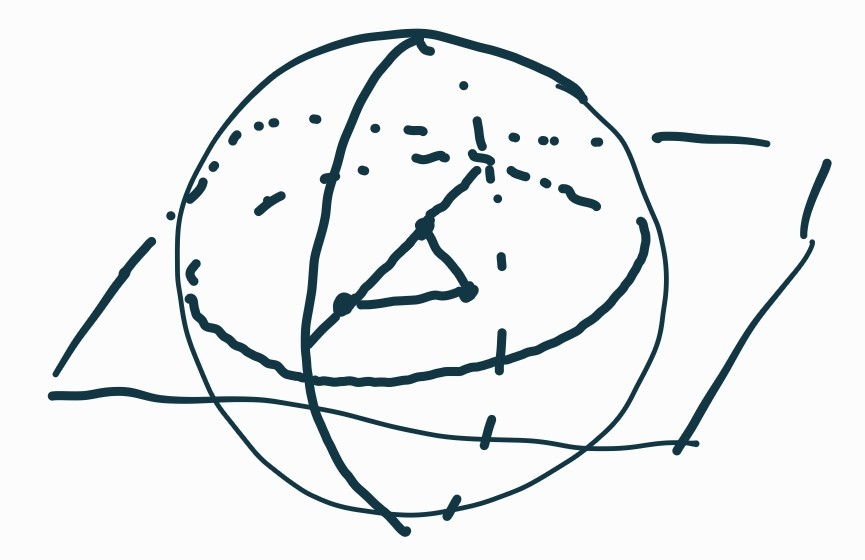
\includegraphics[width=0.4\textwidth]{tempimages/FlatVsConvex.jpg}
	\caption{Flat vs convex set. The ball is the ensemble space. The triangle represents a convex subset. The disc containing the triangle is the flat closure of the triangle. The plane is the affine closure of the triangle.}
\end{figure}


\begin{prop}
	A flat includes all possible affine combinations of elements of $\Ens$ that are contained in $\Ens$. The flat closure of $U \subseteq \Ens$ is the intersection of $\Ens$ with the affine closure of $U$ in the embedding vector space.
\end{prop}

\begin{proof}
	Let $A \subseteq \Ens$ be a flat and let $V$ be the real vector space that embeds $\Ens$. A line between two elements $\ens[a], \ens[b] \in A$ can be extended in $V$ and can be written as $\ens[a] + x \left(\ens[b] - \ens[a]\right)$ with $x \in \mathbb{R}$. Therefore any ensemble that can be written as an affine combination of two ensembles in $A$ is an element of the flat. Recursively, this means that any ensemble that can be written as an affine combination of finitely many ensembles in $A$ is also in the flat. Moreover, since the flat is a closed set, it will also include all its limits. Therefore every affine combination of $A$ that is also an element of $\Ens$ is in $A$, which means $A$ is the intersection of an affine subspace of the embedding vector space and the ensemble space.
	
	Now let $U \subseteq \Ens$ be a set of ensembles. The affine closure of $U$ will be an affine subspace of the embedding vector space. The flat closure will be the intersection of the affine closure with $\Ens$. Since the affine closure is the smallest closed affine subspace that contains $U$, its intersection with $\Ens$ will be the smallest flat that contains $U$, which is the flat closure of $U$.
\end{proof}

\begin{conj}
	An $n$-flat is a simplex if and only if its $3$-flats are simplexes (i.e. triangles).
\end{conj}

\begin{remark}
	In classical discrete ensemble spaces, any flat is a simplex. In classical continuous ensemble spaces, infinite dimensional flats will depend on what limits are allowed. In a quantum ensemble space, if we take three ensembles inside a Bloch ball, the corresponding flat will be a circle. If we take three orthogonal pure states, however, the corresponding flat will be a simplex.
\end{remark}
\end{mathSection}

\subsection{Classical probability contexts}

Now that we have identified the correct closure, we need to find the right characterization of a flat to identify a classical probability context: a set of ensembles that can be characterized by a family of classical probability measures. For finite discrete spaces, we want to recover the notion of a simplex. In a simplex, every element has a single decomposition in terms of extreme points. This characterization does not work in infinite dimensions as there are no extreme points. As we saw before, the pure point probability measures are not, in general, continuous with respect to the topology. The trick, again, is being able to express this lack of multiple decompositions for finite mixtures.

%A classical probability context will be a set of ensembles that we will map to a space of measures. From the ensembles we will need to define the points over which the probability are defined, the spectrum of the context (in analogy to the spectrum of a linear operator). The general idea is that these will be limits of ensembles that become more and more concentrated, which will be characterized using tools from order theory and topology. Once the spectrum is defined, we will use the fraction capacity to define the probability measure over the topology of the spectrum.

%Technical details aside, we want definitions that capture the intuition of spaces of classical probability distributions in a way that works well for infinite dimensional spaces, is compatible with both discrete and continuous classical ensemble spaces but also with measurement contexts in quantum ensemble spaces. It is instructive to go through some of the different attempts to understand why we settled on these definitions, so that one can understand why they work.

\begin{mathSection}
\begin{defn}
	An ensemble is \textbf{decomposable} if it can be expressed as a mixture of two ensembles. An ensemble is \textbf{separately/orthogonally decomposable} if it can be expressed as a mixture of two separate/orthogonal ensembles. An ensemble is \textbf{separately multidecomposable} if it can be expressed as two decompositions where a component of one is separate from both components of the other. That is, $\ens = p \ens[a]_1 + \bar{p} \ens[a]_2 = \lambda \ens[b]_1 +\bar{\lambda} \ens[b]_2$ and either $\ens[a]_1 \separate \ens[b]_j$ or $\ens[a]_2 \separate \ens[b]_j$.
\end{defn}

\begin{figure}[H]
	\centering
	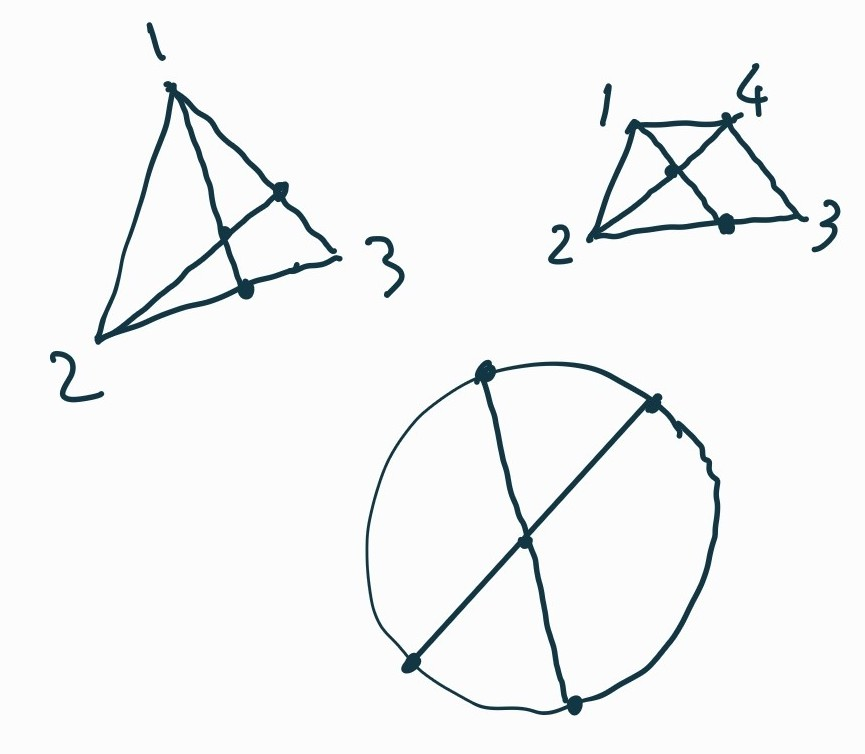
\includegraphics[width=0.4\textwidth]{tempimages/MultipleDecomposition.jpg}
\end{figure}

\begin{remark}
	Take a classical discrete space for three points which is a triangle (simplex). The only three elements that are not decomposable are the extreme points. Mixtures of two points are decomposable and are also separately decomposable in only one way. Mixtures of three points are also separately decomposable, but in multiple ways: as a mixture of $\ens_1$ and a mixture of $\ens_2$ and $\ens_3$, or as a mixture of $\ens_2$ and a mixture of $\ens_1$ and $\ens_3$. Note, however, that they are not separately multidecomposable as the different components are not separate.
	
	Take a Bloch ball for quantum mechanics. All the elements of the surface are not decomposable and they are all pairwise separate. The middle point can be seen as the equal mixture of any pair of opposite points. Therefore the middle point, as well as any other point not on the surface, is not only separately decomposable but also multidecomposable.
	
	To see why we require only one component to be separate from the other two, consider the cut triangle. Here we can have multiple decompositions where not all elements are separate.
\end{remark}

\begin{figure}[H]
	\centering
	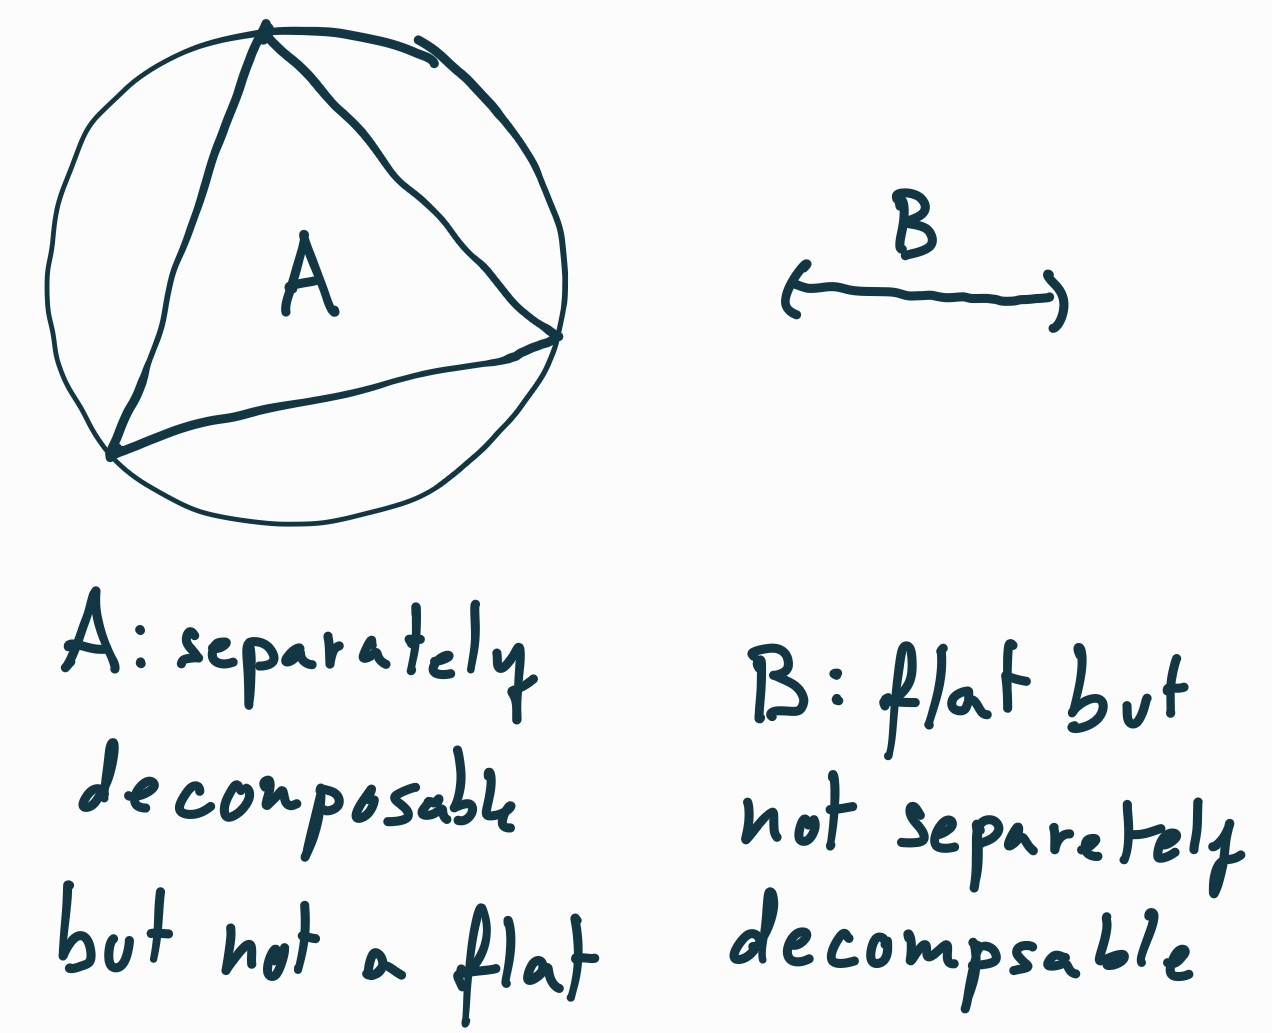
\includegraphics[width=0.4\textwidth]{tempimages/SeparableButNotFlat.jpg}
\end{figure}

\begin{remark}
	A convex set that is separately decomposable is not necessarily a flat (i.e. triangle within a sphere). A flat is not necessarily separately decomposable (i.e. open segment as a whole is a flat, but is not separately decomposable).
\end{remark}

\begin{defn}
	Let $\Ens$ be an ensemble space. A \textbf{classical probability context} is a flat $C \subseteq \Ens$ where each decomposable element in $C$ is separately decomposable in $C$ but not separately multidecomposable in $C$.
\end{defn}

\begin{conj}
	A flat $C \subseteq \Ens$ is a classical probability context if and only if every decomposable element is separately decomposable and mixtures preserve separateness in $C$. That is, if $\ens \separate \ens[a]$ and $\ens \separate \ens[b]$, then $\ens \separate p\ens[a] + \bar{p} \ens[b]$ in $C$ for all $\ens, \ens[a], \ens[b] \in C$ and $p \in [0,1]$.
\end{conj}

\begin{conj}
	A convex subset $U \subseteq \Ens$ is a classical probability context if and only if all finite flats are simplexes.
\end{conj}

\begin{prop}
	Let $C \subseteq \Ens$ be a classical probability context. Let $U \subseteq C$ be a set of ensembles. Then $A=U^\separate=\{ \ens[a] \in C \, | \, \forall \ens \in U, \ens[a] \separate \ens \}$ and $B=(U^\separate)^\separate=\{ \ens[b] \in C \, | \, \forall \ens[a] \in A, \ens[b] \separate \ens[a] \}$ are two probability contexts such that $C = \hull(A \cup B)$.
\end{prop}

\begin{proof}
	First we show that $C$ contains only three types of ensembles: those that are limits of convex mixtures of $A$, those that are limits of convex mixtures of $B$ and those that are limits of convex mixtures of both $A$ and $B$. Any ensemble in $C$ is one of these three types. For $\ens[c] \in C$ to not be a mixture of $A$ or $B$, then $\ens[c]$ cannot be in either $A$ or $B$. This means that it must be separate from both $A$ and $B$. But $B$ contains all the elements that are separate from $A$, which is a contradiction. Since separate multidecomposition is forbidden, an ensemble $\ens$ cannot be written both as a convex combination of $A$ and as a convex combination with an element of $B$. This would yield two decompositions in which one component, the one chosen from $B$, is separate from all the components of the other. This means that an element of $C$ is either a mixture of $A$, a mixture of $B$ or a mixture of both $A$ and $B$.
	
	Now we show that both $A$ and $B$ are convex sets. Since a mixture of $A$ can only be expressed as a mixture of components of $A$, it is separate from all elements of $B$. Therefore $A$ contains all its mixtures. With the same logic, $B$ will contain all its mixtures. The argument works for infinite convex combinations as well. If $\ens = \sum_{i=1}^{\infty} p_i \ens[a]_i$ with $p_i \in [0,1]$ and $\sum_{i=1}^{\infty} p_i = 1$, it can be understood as the limit of the series $\frac{p_1}{P_n} \ens[a]_1 + \frac{\bar{p}_1}{P_n} \sum_{i=2}^{n} p_i \ens[a]_i$ where $P_n = \sum_{i=1}^{n} p_i$. Therefore
	\begin{equation}
		\begin{aligned}
			\ens &= \sum_{i=1}^{\infty} p_i \ens[a]_i = \lim\limits_{n \to \infty}  \sum_{i=1}^{n} \frac{p_i}{P_n} \ens[a]_i = \lim\limits_{n \to \infty} \frac{p_1}{P_n} \ens[a]_1 + \lim\limits_{n \to \infty}\frac{\bar{p}_1}{P_n} \sum_{i=2}^{n} \frac{p_i}{\bar{p}_1} \ens[a]_i = p_1 \ens[a]_1 + \bar{p}_1 \sum_{i=2}^{\infty} \frac{p_i}{\bar{p}_1} \ens[a]_i \\
			&= p_1 \ens[a]_1 + \bar{p}_1 \hat{\ens[a]}_1
		\end{aligned}
	\end{equation}
	where $\hat{\ens[a]}_1 = \sum_{i=2}^{\infty} \frac{p_i}{\bar{p}_1} \ens[a]_i$. Since $\ens$ and $\ens[a]_1$ are elements of the ensemble space, the series converges to $\hat{\ens[a]}_1$, which is in the hull of $A$. It will also be an element of $A$ because multidecompositions are forbidden.
	
	To see that $C$ is the hull of $A$ and $B$, note that all the elements in $C$ that are not already in $A$ or $B$ are the mixtures of $A$ and $B$. These are exactly added when taking the hull of $A \cup B$.
	
	Now we show that $A$ and $B$ are classical probability contexts. First we have to show that they are flats. Let $L$ be the line that connects two elements $\ens[a]_1, \ens[a]_2 \in A$. Take $\ens[a]_3 \in L$. If it is a mixture of $\ens[a]_1$ and $\ens[a]_2$ then it is an element of $A$. If $\ens[a]_1$ is a mixture of $\ens[a]_2$ and $\ens[a]_3$, since $\ens[a]_1$ cannot have a common component with $B$, and $\ens[a]_3$ is a component of $\ens[a]_1$, $\ens[a]_3$ cannot have components in $B$ as well. Therefore $\ens[a]_3$ must be a mixture of elements of $A$. Similarly if $\ens[a]_2$ is a mixture of $\ens[a]_1$ and $\ens[a]_3$. Therefore $A$ is a flat. Similarly, $B$ is a flat.
	
	Now we show that $A$, and by symmetry $B$, is a classical probability context. We have seen that $A$ is a flat. If an element of $A$ is decomposable in $A$ it is also decomposable in $C$ and is therefore separately decomposable in $C$. Because multidecomposability in $C$ is not allowed, it must be separately decomposable into elements of $A$. Lastly, if multidecomposability were allowed in $A$, it would also be allowed in $C$. Therefore it is not allowed in $A$. This means that $A$ is a classical probability context.
\end{proof}

\begin{figure}[H]
	\centering
	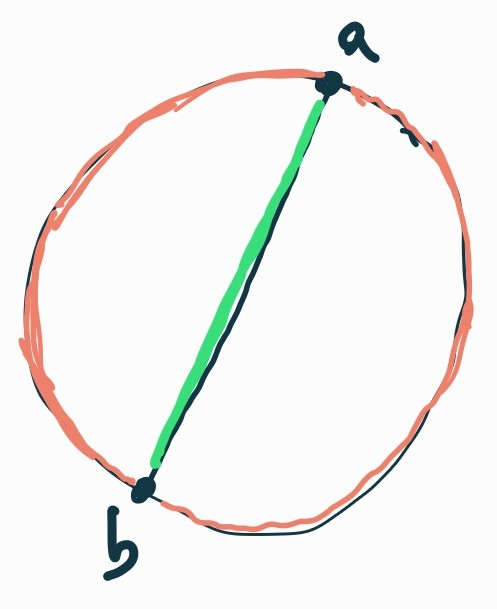
\includegraphics[width=0.25\textwidth]{tempimages/CounterexampleProbabilityContexts.jpg}
	\caption{TODO: make the final picture not go through the center, change the label for the points to $\ens_1$ and $\ens_2$}
\end{figure}

\begin{remark}
	Note that if multiple separate decompositions are not ruled out, the sub-contexts will not include all convex combinations. Take a disk as a convex space. Suppose $U$ is made of two points $\ens_1$ and $\ens_2$. All other points on the surface are separate from both and therefore belong to $A$. Now consider the convex combinations of $\ens_1$ and $\ens_2$. These are not separate from $U$ but they are also not separate from all the other elements on the surface. Therefore they are neither in $A$ nor $B$. Moreover, any other point in the interior can be seen as a convex combination of $\ens_1$ and another element of the surface that is not $\ens_2$. Therefore no point in the interior is in either $A$ or $B$. Thus $A$ and $B$ are not necessarily convex sets if $C$ is not a classical probability context.
\end{remark}

\begin{figure}[H]
	\centering
	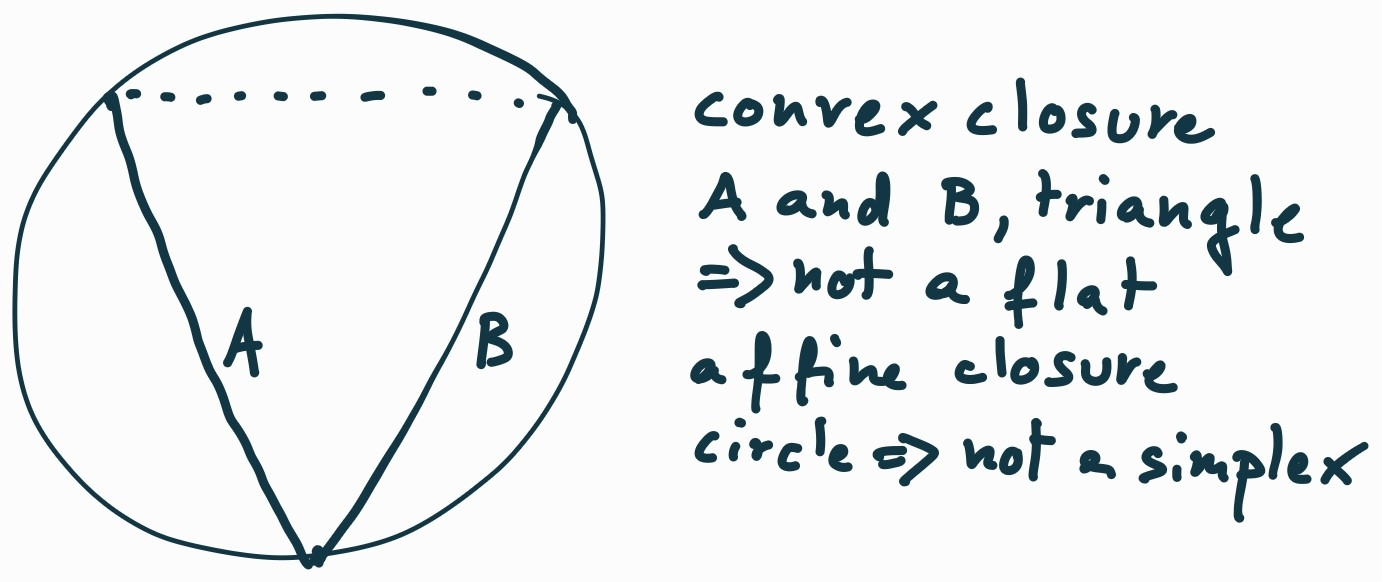
\includegraphics[width=0.75\textwidth]{tempimages/ContextClosureNotContext.jpg}
\end{figure}

\begin{remark}
	While a classical probability context can be decomposed into classical probability contexts whose closure is the original context, the converse is not true. That is, given two classical probability contexts, their convex or flat closure is not in general a classical probability context. Take a disk (the ensemble space) and two lines connecting three points (the two probability contexts). The convex closure is the triangle, which is not a flat as it misses some affine combinations. The flat closure is the disk, which is not a probability context.
\end{remark}

\begin{conj}
	Let $A, B \subseteq \Ens$ be two classical probability contexts. Then their flat closure and convex closure coincide if and only if these closures are a classical probability context.
\end{conj}

\begin{conj}
	The defining property of a classical probability context is exactly that property that allows $A$ and $B$ so constructed to be convex sets whose closure is $C$.
\end{conj}

\begin{prop}
	Let $C \subseteq \Ens$ be a classical probability context. Let $\mathfrak{L}$ be the lattice of $\separate$-subspaces. Then the fraction capacity is an additive set function on the lattice. That is, for all $\ens \in C$ and $A, B \in \mathfrak{L}$ such that $A \cap B = \emptyset$,  $\fcap_{\ens}(A \vee B) = \fcap_{\ens}(A) + \fcap_{\ens}(B)$.
\end{prop}

\begin{proof}
	Let $A, B\in \mathfrak{L}$ such that $A \cap B = \emptyset$. Then $A$ is separate from $B$. Therefore $A \vee B$ is a classical probability context that is the convex closure of two separate probability contexts. Therefore, as we saw in a previous proof, $A \vee B$ consists of convex combinations of $A$, which are all in $A$, of convex combinations of $B$, which are all in $B$, and of convex combinations of both, which are in neither $A$ nor $B$.
	
	We want to show that $\fcap_{\ens}(A \vee B) = \fcap_{\ens}(A) + \fcap_{\ens}(B)$ if $\ens \in A \vee B$. Let $\ens \in A \vee B$ be an ensemble that is the mixture of elements of $A$. Then $\ens \in A$ and it has no components in $B$. Therefore $\fcap_{\ens}(A \vee B) = 1$ and $\fcap_{\ens}(A) = 1$ while $\fcap_{\ens}(B) = 0$. This means $\fcap_{\ens}(A \vee B) = 1 = 1 + 0 = \fcap_{\ens}(A) + \fcap_{\ens}(B)$. If $\ens$ is a mixture of elements of $B$, we get the same conclusion. The last case is when $\ens$ is a mixture of elements of $A$ and $B$. That is, $\ens = \sum_i p_i \ens[a]_i + \sum_j \lambda_j \ens[b]_j$ with $\ens[a]_i \in A$, $\ens[b]_j \in B$, $p_i, \lambda_j \in [0,1]$ and $\sum_i p_i + \sum_j \lambda_j = 1$. By definition of fraction capacity, $\sum_i p_i \leq \fcap_{\ens}(A)$. Suppose $\sum_i p_i < \fcap_{\ens}(A)$. Then there is $\hat{\ens[a]} \in A$ such that $\ens = \sum_i p_i \ens[a]_i + p \hat{\ens[a]} + \lambda \ens[c]$ for some $p,\lambda \in [0,1]$ and $\ens[c] \in A \vee B$. But then $\ens$ would be separately multidecomposable, which is a contradiction since it is an element of a classical probability context. Therefore $\sum_i p_i = \fcap_{\ens}(A)$. Similarly, we find that $\sum_j \lambda_j = \fcap_{\ens}(B)$. Since $\sum_i p_i + \sum_j \lambda_j = 1$, $\fcap_{\ens}(A) + \fcap_{\ens}(B) = 1 = \fcap_{\ens}(A \vee B)$ for all $\ens \in A \vee B$.
	
	Now let $\ens \in C$. We have $(A \vee B)^\separate \in \mathfrak{L}$ and $(A \vee B) \cap (A \vee B)^\separate = \emptyset$. Therefore $\fcap_{\ens}(C) = \fcap_{\ens}(A \vee B)+ \fcap_{\ens}((A \vee B)^\separate)$. Note that $\ens$, in general, is a convex combination of elements of $A\vee B$ and $(A \vee B)^\separate$. Components in $A \vee B$ are convex combinations of elements of $A$ and $B$, which also disjoint. Therefore $\ens$ is a convex combination of elements of $A$, $B$ and $(A \vee B)^\separate$, which are pairwise disjoint. As before, since multidecomposability is forbidden in a classical probability context, the sum of the coefficients for each part will have to match the fraction capacity of its subcontext. Therefore $\fcap_{\ens}(A) +  \fcap_{\ens}(B) + \fcap_{\ens}((A \vee B)^\separate) = \fcap_{\ens}(C) = \fcap_{\ens}(A \vee B) + \fcap_{\ens}((A \vee B)^\separate)$. Thus $\fcap_{\ens}(A \vee B) = \fcap_{\ens}(A) +  \fcap_{\ens}(B)$ for all $\ens \in C$.
\end{proof}
\end{mathSection}

\subsection{Spectrum of a classical probability context}

To recover classical probability distributions, we need to recover the possible cases (i.e. the sample space) and the events (i.e. the $\sigma$-algebra) over which the probability distributions are defined. These are not necessarily states. For example, in the countinuous classical case, the sample space corresponds to the sets of possible values of position and momentum (i.e. the symplectic manifold over which the values are defined). In quantum mechanics, the sample space is the range of possible values defined by an observable (i.e. the spectrum of the operator). The goal here is to identify a single physically meaningful construction that will be able to work for all these cases.

Intuitively, we are taking ensembles and decomposing them into mixtures of ensembles with narrower and narrower spread. The points over which the classical distributions are defined are limits where the spread goes to zero. Note, however, that the limit of sequences with narrower and narrower spread will not, in general, be itself an ensemble. For example, we can imagine a sequence of uniform distributions over $[-\frac{1}{i}, \frac{1}{i}]$. As $i$ increases, the spread will converge to the single value $0$, though the sequence of ensembles will not converge to an ensemble. Similarly, we can imagine a sequence of density matrices, or even wave-functions, for the quantum case. The points, then, should be understood as a convenient tool for representation and calculation, not as physically realizable objects. What is physically realizable, at least conceptually in the model, is the sequence of finer and finer decomposition at an arbitrary level of precision. That is, conceptually we are not starting from the sample space (i.e. the possible idealized values) and then constructing probability distributions on top; we start with a set of ensembles, which are the physical objects we are studying, and obtain the points and the corresponding probability distributions as the limit of recursive decomposition.

Mathematically, the construction uses the notion of subspaces defined in \ref{pm_es_subspaceSection} applied to separateness. We use separateness to construct sets of ensembles that share the same support. These are the $\separate$-subspaces and are constructed by looking for pairs of sets such that all the elements of one are separate from all the elements of the other. These subspaces form a lattice: they have a partial order according to set inclusion. Therefore we can find sequences of subspaces that become more and more refined, whose elements have a narrower and narrower support. Using a standard technique in topology, the points are identified by a collection of subspaces (called ultrafilters) that become smaller and smaller. A limiting sequence can be understood as taking an element from each of these shrinking subspaces. We call the set of all these points the spectrum of the context.

Every subspace can then be understood as a set of limits, a set of ultrafilters, that are open sets in the topology of the spectrum. The topology is the one generated by those sets.

\begin{mathSection}
\begin{defn}
	Given a classical probability context $C \subseteq \Ens$, the \textbf{spectrum} $\sigma(C)$ is the set of equivalence classes of sequences of ensembles that eventually become separate from each other. More rigorously, given a probability context, the spectrum is the collection of the ultrafilters of the lattice of $\separate$-subspaces $\mathfrak{L}^\separate(C)$. The spectrum of each $\separate$-subspace is given by $\sigma(A) \mapsto \{ x \in \sigma(C) \, | \, A \in x \}$. The standard topology of the spectrum is the one generated by the spectra of all $\separate$-subspaces (i.e. $\sigma(\mathfrak{L}^\separate(C))$.
\end{defn}

\begin{prop}
	Let $C \subseteq \Ens$ be a classical probability context and $\sigma(C)$ its spectrum. Then the following are true:
	\begin{enumerate}
		\item $A \subseteq B$ if and only if $\sigma(A) \subseteq \sigma(B)$
		\item $\exterior(\sigma(A)) = \sigma(A^{\separate})$
		\item $\partial \sigma(A) = \{ x \in \sigma(C) \, | \, A \notin x, A^{\separate} \notin x \}$
		\item $\sigma(A)^{\complement} = \overline{\sigma(A^{\separate})}$
		\item $\sigma(\bigwedge_{i \in I} A_i) = \interior\left(\bigcap_{i \in I} \sigma(A_i)\right)$
		\item $\sigma(\bigvee_{i \in I} A_i) = \interior\left(\overline{\bigcup_{i \in I} \sigma(A_i)}\right)$
		\item if $U$ open, then $U = \bigcup_{i \in I} \sigma(A_i)$ for some family of $A_i \in \mathfrak{L}^\separate(C)$
	\end{enumerate}
\end{prop}

\begin{proof}
	For 1, since all $x \in \sigma(C)$ are upward closed, $A \in x$ means $B \in x$ as well. Therefore if $x \in \sigma(A)$ then $x \in \sigma(B)$, which means $\sigma(A) \subseteq \sigma(B)$. Conversely, if $\sigma(A) \subseteq \sigma(B)$ then all downward sets of $\mathfrak{L}^\separate(C)$ that contain $A$ must also contain $B$, which means $B \supseteq A$.
	
	For 2 and 3, note that $\sigma(A) = \{ x \in \sigma(C) \, | \, A \in x \}$ and therefore $\sigma(A)^{\complement} = \{ x \in \sigma(C) \, | \, A \notin x \}$. Since $\sigma(A)$ is an open set, $\sigma(A)^{\complement} = \exterior(\sigma(A)) \cup \partial \sigma(A)$. Now consider $\sigma(A^{\separate})$. This is an open set and it is disjoint from $\sigma(A)$. In fact, if $x \in \sigma(A) \cap \sigma(A^{\separate})$ then $A, A^{\separate} \in x$. But this would mean that $\emptyset \in x$, which can't be because $x$ is a proper filter and cannot contain $\emptyset$. Since $A^{\separate}$ is the largest $\separate$-subspace that is separate from $A$, there is no set in $\sigma(\mathfrak{L}^\separate(C))$ that is larger than $A^{\separate}$ and still disjoint from $A$. Therefore $\sigma(A^{\separate}) = \exterior(\sigma(A))$. We have $\partial \sigma(A) = \sigma(C) \setminus (\interior(\sigma(A))\cup\exterior(\sigma(A))) = \{ x \in \sigma(C) \, | \, A \notin x, A^{\separate} \notin x \}$.
	
	For 4, since $\sigma(A)$ is an open set, the complement is the closure of the exterior. Therefore, given 2, $\sigma(A)^{\complement} = \overline{\sigma(A^{\separate})}$.
	
	For 5, consider $\bigwedge_{i \in I} A_i$. This is the largest $\separate$-subspace that is contained by all $A_i$. Then, given 1, $\sigma\left(\bigwedge_{i \in I} A_i\right)$ must be the largest open set that is contained by all $\sigma(A_i)$. This corresponds to $\interior\left(\bigcap_{i \in I} \sigma(A_i)\right)$.
	
	For 6, we have
	\begin{align*}
		\sigma(\bigvee_{i \in I} A_i) &= \exterior(\exterior(\sigma(\bigvee_{i \in I} A_i))) = \exterior(\sigma((\bigvee_{i \in I} A_i)^{\separate})) = \exterior(\sigma(\bigwedge_{i \in I} A_i^{\separate})) \\
		&= \exterior(\interior(\bigcap_{i \in I} \sigma(A_i^{\separate}))) = \exterior(\bigcap_{i \in I} \sigma(A_i^{\separate})) =  \\
		&= \exterior\left(\bigcap_{i \in I}\overline{\sigma(A_i)}^{\complement}\right) = \exterior\left(\left(\bigcup_{i \in I}\overline{\sigma(A_i)}\right)^{\complement}\right) \\
		&= \interior\left(\bigcup_{i \in I}\overline{\sigma(A_i)}\right)
	\end{align*}
	For the last step, note that the union of the closure is not necessarily the closure of the union, but they have the same interior. (TODO: check that the ext of int is really ext in the second line)
	
	For 7, note that an open set $U$ is generated from $\sigma(\mathfrak{L}^\separate(C))$ through finite intersection and arbitrary union. Note that the finite intersection of open sets is an open set, so we have $\bigcap_{i \in I} \sigma(A_i) = \interior\left(\bigcap_{i \in I} \sigma(A_i)\right) = \sigma(\bigwedge_{i \in I} A_i)$. Therefore the finite intersection corresponds to a $\separate$-subspace. This means that we can can generate all open sets with arbitrary unions of sets from $\sigma(\mathfrak{L}^\separate(C))$.
\end{proof}

\begin{remark}
	Note how the infinite joins/meets on the lattice of the $\separate$-subspaces do not correspond to the infinite operations on the lattice of the topology or of the Borel sets. For example, suppose we are taking the lattice of probability measures defined over the interval $[0,1]$ that are absolutely continuous with respect to the Lebesgue measure. Each $\separate$-subspace will correspond to a set of measures whose support lives in a particular region. A singleton will not correspond to any subspace as it cannot support an absolutely continuous measure. Therefore, if we take all the $\separate$-subspaces of all measures that have $1/2$ within the support, the intersection of all those subspaces will be the empty set, which is a $\separate$-subspace. However, the intersection of the sets representing their support is the singleton $\{1/2\}$, which is not the empty set. However, its interior is the empty set.
	
	The fact that a single probability measure is an equivalence class of probability densities is related to this distinction. Consider a uniform distribution over $[0,1]$. The related probability density can be understood as a constant between those values and zero everywhere else. However, the same constant over $[0,1/2) \cup (1/2,1]$ will also work. That is, the same element of the ensemble space can be represented in different ways as a function over the spectrum.
\end{remark}
\end{mathSection}

\subsection{Probability measures from classical probability contexts}

We now show that each ensemble in a classical probability context can be understood as a probability measure over the spectrum of the context. That is, each ensemble can either be understood as a convex combination of smaller and smaller components that are separate from each other.

\begin{mathSection}
\begin{thrm}
	Let $C \subseteq \Ens$ be a probability context and $\ens \in C$ be an ensemble in the context. The set function $p^*_{\ens} : \textsf{T}_{\sigma(C)} \to[0,1]$, defined such that $p^*_{\ens}(U) = \inf(\{ \fcap_{\ens}(A) \, | \, \sigma(A) \supseteq U \})$, is a topological measure. Therefore an ensemble in a classical probability context can be represented by a unique measure over its spectrum that is continuous with respect to its topology.
\end{thrm}

\begin{proof}
	Since $p^*_{\ens}$ is finite, it is locally finite. We need to show that is topologically additive. If $U$ is a generic open set, then we are looking for the smallest subspace $A$ such that $\sigma(A) \subseteq U$. If $U$ corresponds to a $\separate$-subspace $A$, that is $U = \sigma(A)$, then $p^*_{\ens} = \fcap_{\ens}(A)$. If not, $U$ can still be written as the union of the spectra of a family of subspaces. That is, $U = \bigcup_{i \in I} \sigma(A_i)$ for some family of $A_i \in \mathfrak{L}^\separate(C)$. The smallest subspace that contains them all, then is the join of all $A_i$. Therefore we have $p^*_{\ens}(U) = p^*_{\ens}(\sigma(A)) = p^*_{\ens}(\sigma(\bigvee_{i \in I} A_i)) = p^*_{\ens}\left(\interior\left(\overline{\bigcup_{i \in I} \sigma(A_i)}\right)\right)$. Lastly, let $U_i$ be a family of disjoint open sets and let $A_i$ be the corresponding smallest subspaces such that $\sigma(A_i) \supseteq U_i$. Since $U_i$ are disjoint, $A_i$ will also be disjoint, and therefore they will be separate. But the fraction capacity is additive across separate subspaces. We have $\sum_{i \in I} p^*_{\ens}(U_i) = \sum_{i \in I} \fcap_{\ens}(A_i) = \fcap_{\ens}(\bigvee_{i \in I} A_i) = p^*_{\ens}\left(\interior\left(\overline{\bigcup_{i \in I} \sigma(A_i)}\right)\right) = p^*_{\ens}\left(\interior\left(\overline{\bigcup_{i \in I} U_i}\right)\right)$. Therefore $p^*_{\ens}$ is a topological measure.
	
	The measure, then, can be extended uniquely to the whole $\sigma$-algebra, since the measure is finite.
	
	Lastly, we need to show that two different ensembles will correspond to two different measures. Let $\ens[a],\ens[b] \in C$ be two distinct ensembles in the probability context. TODO
\end{proof}
\end{mathSection}

\begin{conj}
	A convex subset $U \subset \Ens$ is a classical probability context if and only if it is the subset of probability measures of a vector space of measures over a sample space $\Omega$.
\end{conj}

We now want to show that, in standard ensemble spaces, we recover the standard notions of probability.

\begin{mathSection}
\begin{prop}
	Let $\Ens$ be a discrete classical ensemble space over a set $X$ of outcomes. Then $\Ens$ is a probability context, the spectrum is $X$ and its topology is the discrete topology. The probability measures over the spectrum recover the original probability measures.
\end{prop}

\begin{proof}
	Let $\Ens$ be a discrete classical ensemble space. The whole space is a flat as it contains all its affine combinations. Note that two ensembles are separate if and only if they have disjoint support. Suppose $\ens = p \ens[a]_1 + \bar{p} \ens[a]_2 = \lambda \ens[b]_1 + \bar{\lambda} \ens[b]_2$. Then the union of the support of each pair must be the same. Therefore the support of at least one element of each pair must overlap with the support of another element of another pair. This means that separate multidecomposability is not allowed. Therefore $\Ens$ is a classical probability context.
	
	Since ensembles are separate if and only if they have disjoint support, the $\separate$-subspace of a subset $A \subseteq \Ens$ of ensembles corresponds to all ensembles whose support is a subset of the union of the supports of the elements of $A$. Each $\separate$-subspace, then, is associated to one unique subset $U \subseteq \Omega$ of the sample space. Given that for any subset $U$ we can find a measure whose support is $U$, every subset corresponds to a unique $\separate$-subspace. If the support of a measure is a subset of $U$, it will also be a subset of any other set $V \supseteq U$. Therefore the ordering of the lattice of $\separate$-subspaces is the same as inclusion on the lattice of supports. The two lattices are isomorphic.
	
	Since the singletons are elements of the lattice, all ultrafilters are principal, meaning that they are all of the form $\uparrow\mathclose{x} = \{A \in \mathfrak{L}^\separate(C) \, | \, \{x\} \in A\}$ where $x \in \Omega$ is an element of the sample space. Therefore the sample space and the spectrum coincide. Each singleton is an open set, since it is an element of the lattice. The topology is therefore the discrete topology.
	
	Now consider $p^*_{\ens}(\{x\})$ for some $x \in X$. Since $\{x\}$ is a $\separate$-subspace, $p^*_{\ens}(\{x\}) = \fcap_{\ens}(\{x\}) = \size_{\ens}(x)$. Note that the ensemble $\ens$ corresponds to a probability measure $p$ which can be written as a convex combination $\ens = \sum_{x_i \in X} p(\{x_i\}) x_i$. Given an $x \in X$, then, $p(\{x\})$ is the greatest mixing coefficient that can be associated to $x$ in a convex combination, which corresponds to the fraction capacity. Therefore $p^*_{\ens}(\{x\}) = p(\{x\})$ for all $x \in X$, which means the two measures are the same.
\end{proof}
\end{mathSection}

\begin{prop}
	Let $\Ens$ be a continuous classical ensemble space over a symplectic manifold $X$. Then $\Ens$ is a probability context, the spectrum is $X$ and its topology is locally the standard topology of $\mathbb{R}^n$.
\end{prop}

\begin{proof}
	Let $\Ens$ be a continuous classical ensemble space. The whole space is a flat as it contains all its affine combinations. Note that two ensembles are separate if and only if they have disjoint support. Suppose $\ens = p \ens[a]_1 + \bar{p} \ens[a]_2 = \lambda \ens[b]_1 + \bar{\lambda} \ens[b]_2$. Then the union of the support of each pair must be the same. Therefore the support of at least one element of each pair must overlap with the support of another element of another pair. This means that separate multidecomposability is not allowed. Therefore $\Ens$ is a classical probability context.
	
	Since ensembles are separate if and only if they have disjoint support, the $\separate$-subspace of a subset $A \subseteq \Ens$ of ensembles corresponds to all ensembles whose support is a subset of the union of the supports of the elements of $A$. Each $\separate$-subspace, then, is associated to a subset $U \subseteq \Omega$ of the sample space. If the support of a measure is a subset of $U$, it will also be a subset of any other set $V \supseteq U$. Therefore the ordering of the lattice of $\separate$-subspaces is the same as inclusion on the lattice of supports. The two lattices are isomorphic. Unlike the discrete version, in the continuous case not all sets can be the support of a probability measure that is part of the ensemble space. For example, a set of measure zero with respect to the Liouville measure cannot support a probability measure absolutely continuous with respect to the Liouville measure.
	
	Recall that the support of a probability measure is the smallest closed set such that $p(A) = 1$. Given that the ensemble space is formed by probability measures that are absolutely continuous with respect to the Liouville measure, the measure over the support is equal to the measure of the interior. Therefore a set $U$ corresponds to a $\separate$-subspace if and only if the $U = \overline{\interior(U)}$. Given that the measure is zero on the boundary, we can really think of each $\separate$-subspace as corresponding to those open sets that are the interior of their own closure.
	
	Note that any open coordinate ball is the interior of its closure. Since any point can be recovered as the limit of a decreasing sequence of open coordinate balls, every $x \in X$ corresponds to an ultrafilter of $\mathfrak{L}^\separate(C)$. That is, the ultrafilters are not principal because there is no absolutely continuous measure that has support only on $x$, but they are still associated with a single point: they corresponds the supports that contain an open neighborhood of $x$. Each $\separate$-subspace, then, corresponds to the interior of the support as there is no open neighborhood of limit points. Since $\mathfrak{L}^\separate(C)$ contains all open ball, the topology generated is the one of the manifold $X$.
	
	Now consider $p^*_{\ens}(U)$ for some open set $U \subseteq X$. Since $p^*_{\ens}(U) = p^*_{\ens}(\interior(\overline{U}))$ and $\interior(\overline{U})$ corresponds to a $\separate$-subspace, noted $A(\interior(\overline{U}))$, $p^*_{\ens}(U) = \fcap_{\ens}(A(\interior(\overline{U})))$. Given an absolutely continuous probability measure $p$ and a set $U$, we can write $p = p(U) \frac{\left.p\right|_{U}}{p(U)} + p(U^{\complement}) \frac{\left.p\right|_{U^{\complement}}}{p(U^{\complement})}$, which is a convex combinations of two absolutely continuous probability measures. Moreover, $p(U)$ corresponds to the greatest mixing coefficient that can be associated to a probability measure with support $U$. Therefore $p(U) = \fcap_{\ens}(A(\interior(\overline{U}))) = p^*_{\ens}(U)$, which means $p = p^*_{\ens}$.
\end{proof}

\begin{remark}
	TODO: organize. There are different types of limits. One limit of convex combinations. Physically, these are mixtures over infinitely many elements. Limit of ensemble sequences. Physically, these are sequences of ensembles, taken one after the other, for example in temporal succession. Limits of ensembles taken from $\separate$-subspaces strictly included into each other. This is the limit of ensemble that are finer and finer.
\end{remark}

We now want to show the relationship between classical probability context for classical and quantum ensembles spaces. For classical ensemble spaces the connection is simple: every classical ensemble space is classical probability context. The reverse is not true. We could have, for example, an ensemble space that is exactly like the discrete classical one except for the entropy of the pure states, which are all assumed to be zero in a discrete classical ensemble space. The convex space structure would be exactly the same, but the entropy wouldn't match. We could also have a space of probability functions defined on a space that is not symplectic. This would be classical probability contexts, but not a space of classical ensembles.

\begin{conj}
	Discrete and continuous classical ensemble spaces are classical probability contexts.
\end{conj}

%\begin{proof}
%	Let $\Ens$ be a classical probability space and let $\mu, \nu \in \Ens$ be probability measures on some space $\Omega$. The space of probability measures is a subset of the space of signed measures. This space can be equipped with an inner product. The space of signed measures with support $U \subseteq \Omega$ forms a subspace. This means that, if we can find a $U \subseteq \Omega$ such that both $\mu(U) \neq 0$ and $\nu(U) \neq 0$, we can find a probability measure that is a component of both. That is, two probability measures that have overlapping support have a common component. Conversely, given that convex combination can only expand the support of measures, two probability measures that have no overlapping support have no common components. (TODO: if all measure are allowed, we may get also measures we do not want - Dirac measures, measures that have no continuous derivative. If not all measures are allowed, we have no existence of a measure that can be a component, and therefore there may be overlapping measures that have no common components.)
	
%	Now, suppose $\ens \separate \ens[a]$ and $\ens \separate \ens[b]$. This means that the support of $\ens$ is disjoint from the support of both $\ens[a]$ and $\ens[b]$, which will also be disjoint from the support of any mixture of $\ens[a]$ and $\ens[b]$ since the support of the mixture will be the union of the individual supports. This means that $\ens$ will be separate from all mixtures of $\ens[a]$ and $\ens[b]$. The property holds, then, in any classical ensemble space.
%\end{proof}

A quantum ensemble space, however, does not allow a description in terms of classical probability precisely because it allows separate multidecompositions.

\begin{prop}
	A quantum ensemble space is not a classical probability context.
\end{prop}

\begin{proof}
Let $\Ens$ be a quantum ensemble space. Let $A \subseteq \Ens$ the space of mixtures of a two dimensional subspace (i.e. a Bloch sphere) and consider the states $x^+$, $x^-$, $z^+$, and $z^-$, which are points on the surface that form a square. These are all separate ensembles. We have $\frac{1}{2} x^+ + \frac{1}{2} x^- = \frac{1}{2} z^+ + \frac{1}{2} z^-$ therefore the space allows separate multidecomposition and is not a classical probability context.
\end{proof}

However, given a maximal set of commuting observables, we can define a classical probability context as the set of all mixed states that commute with all the observables. This makes the spectrum of all the density operator coincide with the product of the spectra of all commuting observables, and therefore those mixed states can be characterized by a measure over the spectra.

\begin{conj}
	Let $\Ens$ be a quantum ensemble space. Let $O_i$ a maximal set of commuting observables. Let $C \subseteq \Ens$ be the set of mixed state that commute with all $O_i$. Then $C$ is a classical probability context.
\end{conj}

\section{Statistical properties and quantities}

Given our ensembles first approach, we define statistical quantities as linear functions of ensembles. The idea is that a statistical quantity represents an expectation over ensembles. The possible value of the quantities will need to be recovered with constructions that mimic spectral theory, though we will not want to talk about eigenstates and eigenvalues in the general case since these are not properly defined for a continuous quantity.

\subsection{Properties and quantities}

These definitions extend the notion of properties and quantities that we defined for an experimental domain. In that case, we simply required that a property we a continuous map to a set of possible values for the property. For a statistical property, the set of values are a topological convex space, so that the property allows statistical mixing. For a quantity is simply a linearly ordered property, which in this case will always be a real valued quantity. The convexity, the averaging operation, fills in the gaps in the linear order in case that not all intermediate values can be obtained.

\begin{defn}
	A \textbf{statistical property}, or simply property, is an attribute that allows statistical handling. Formally, it is a continuous map $F : \Ens \to \mathcal{Q}$ where $\mathcal{Q}$ is a convex topological space such that $F(p \ens_1 + \bar{p} \ens_2) = p F(\ens_1) + \bar{p} F(\ens_2)$.
	
	A \textbf{statistical quantity}, or statistical variable, or simply variable, is a numerical statistical property. That is, it is a continuous linear real valued operator $F : \Ens \to \mathbb{R}$.
\end{defn}

\begin{justification}
	This definition extends the general definition of properties and quantities we already gave to the statistical case. As before, continuity is required since verifying the value of the quantity corresponds to verifying that we are dealing with a specific subset of ensembles.
	
	The ability to create convex combinations corresponds to the ability to create statistical averages. Therefore $\mathcal{Q}$ must be a convex set. Given that preparations are assumed to be independent, the a mixture of the preparation will produce a mixture of the properties according to the same fractions. 
	
	Quantities are simply properties that are linearly ordered. The ability to create convex combinations becomes the ability to take weighted averages of the quantities. Regardless of whether one starts from integers, rationals or real valued quantities, the statistical averages will, in general, be a real number.
	
	Note that the numerical value cannot be infinite. The only way to measure infinity is if the measured average keeps increasing in time. This would be a contradiction on the assumption that the ensemble represent a reproducible collection of preparations.
\end{justification}

\begin{remark}
	Note that variables will have a contiguous range on the ensembles because, given two ensembles with different values, we can mix them to obtain any intermediate value. This does not mean that the variable can take all possible values on pure states. For example, the number of particles in a pure state will necessarily be a non-negative integer, but we can mix those to create ensembles that have non-integer average number of particles.
\end{remark}

\begin{coro}
	A set of statistical quantities $\{F_i\}_{i \in I}$ can be collected into a single statistical property $F : \Ens \to \mathbb{R}^I$ where $F(\ens) = \{F_i(\ens)\}_{i \in I}$.
\end{coro}

Here we show that statistical quantities recover the standard random variables of classical mechanics and observables of quantum mechanics.

\begin{prop}
	Let $\Ens$ be a classical probability space. Then each statistical quantity is the expectation of a random variable and vice-versa.
\end{prop}

\begin{proof}
	Let $\Ens$ be an ensemble space where each ensemble is a probability measure $\mu$ over some sample space $\Omega$. Let $f : \Omega \to \mathbb{R}$ be a random variable, then the expectation $F(\mu) = \int_{\Omega} f d\mu$ is a statistical quantity. Conversely, let $F : \Ens \to \mathbb{R}$ be a linear functional of the measures. Then, by Riesz representation theorem, we can write $F(\mu) = \int_{\Omega} f d\mu$ from some $f : \Omega \to \mathbb{R}$.
\end{proof}

\begin{conj}
	Let $\Ens$ be a quantum ensemble space. Then each statistical quantity is the expectation of an observable and vice-versa.
\end{conj}

\begin{proof}
	TODO: need to find a quantum correspondent of the Riesz representation theorem.
\end{proof}

\subsection{Quantifiable spaces and locally convex vector spaces}

A common case is when all ensembles are identifiable by a set of statistical variables.

\begin{defn}
	A \textbf{quantifiable} ensemble space is an ensemble space where each ensemble can be identified by a set of statistical variables. That is, there is family of statistical variables $F_i : \Ens \to \mathbb{R}$ such that, given $\ens_1, \ens_2 \in \Ens$, $F_i(\ens_1) = F_i(\ens_2)$ for all $i$ if and only if $\ens_1 = \ens_2$. Moreover, the topology is generated by those variables.
\end{defn}

\begin{remark}
	Ideally, we would want to show that the topology must be generated by those variables instead of imposing it.
\end{remark}

\begin{prop}
	A statistical variable $F$ induces a semi-norm on the vector space that embeds $\Ens$.
\end{prop}

\begin{proof}
	Let $F$ be a variable on $\Ens$ and let $V$ be the vector space that embeds $\Ens$. Extend $F$ on $V$ such that $F(a\ens) = |a| F(\ens)$. Then, according to the definition given after 1.1 in \url{https://personal.math.ubc.ca/~cass/research/pdf/TVS.pdf} $F$ is a semi-norm.
\end{proof}


\begin{prop}
	A quantifiable ensemble space embeds continuously into a Hausdorff locally convex topological vector space.
\end{prop}

\begin{proof}
	The topology of the ensemble space is generated by the statistical variables, which induce semi-norms on the ambient vector space. This means that the topology of the vector space is generated by a countable set of semi-norms, and is therefore a locally convex topological vector space. See Prop 2.2 in \url{https://personal.math.ubc.ca/~cass/research/pdf/TVS.pdf}.
	
	The statistical variables fully identify each ensemble, which means that, if two elements are different, one semi-norm will give a non-zero value for the distance function associated with it. This means that the topology is Hausdorff. See Prop 2.6 in \url{https://personal.math.ubc.ca/~cass/research/pdf/TVS.pdf}.
\end{proof}

\begin{coro}
	A quantifiable ensemble spaces is fully determined by countably many statistical variables.
\end{coro}

\begin{proof}
	The topology of an ensemble space is second countable. A Hausdorff second countable locally convex topological vector space can always be generated by countably many semi-norms.
\end{proof}

\begin{remark}
	Note that we are missing completeness in terms of the semi-norms to obtain a Fr\'echet space. It is not clear whether this is required since, for example, $L^1(\mathbb{R}^{2n}) \cap C(\mathbb{R}^{2n})$ is not Fr\'echet.
\end{remark}

\begin{conj}
	Discrete/continuous classical ensemble spaces and quantum ensemble spaces are quantifiable.
\end{conj}

\begin{proof}
	For discrete classical spaces, the expectation of the indicator of each extreme point defines a countable set of quantities that fully identifies the distribution.
	
	For continuous classical spaces, note that $L^1(\mathbb{R}^{2n})$ is a Hausdorff locally convex topological spaces.
	
	TODO Quantum (note that we are looking at the space of density operators with finite expectation value for position and momentum).
\end{proof}

\begin{conj}
	If all ensembles can be connected by linear transformations parameterized by real quantities, then the ensemble is quantifiable.
\end{conj}

\begin{remark}
	Not clear whether this is true. The idea is that the time interval can be used to define variables. A more sophisticated conjecture may look at the space of generators of Lie groups. This would link the topology of time to the topology of the ensemble space. If the topology of time is not that of the real numbers, then, the ensemble space must change significantly.
\end{remark}

\subsection{Macrostates and thermodynamics}

In this section we try to recover some elements of thermodynamics on the generalized ensemble space. We want to recover Gibbs' thermodynamics, which means an equation of state in terms of extensive quantities. Instead of extensive quantities, we are going to use statistical quantities. Note that the idea that all extensive quantities are statistical (i.e. the average during mixing) seems to work. The energy and the number or particles average during mixture. The idea that volume averages during mixture can be understood as the system oscillating between the different volumes defined by the components. It also seems that intensive quantities do not average during mixing. Temperature, for example, is only defined on equilibria (i.e. of Boltzmann distributions) and the mixture of two equilibria at different temperature is not an equilibrium. Still, we would need a general proof, which would require the notion of product spaces (i.e. intensitive/extensive quantities represent system/subsystem relationship).

\begin{defn}
	Let $\Ens$ be an ensemble space. Let $F : \Ens \to \mathcal{Q}$ be a statistical property. The \textbf{coarse graining} of $\Ens$ over $F$ is the set $\mathcal{M} \subseteq \Ens$ represented by the ensemble that maximize the entropy for each fixed value of the property. That is, there exists a map $\psi : \mathcal{Q} \to \mathcal{M}$ such that $F(\psi(x)) = x$ and $S(\psi(x)) \geq \ens$ for all $\ens \in \Ens$ such that $F(\ens) = x$. The \textbf{equation of state} is the map $S(x) \mapsto S(\psi(x))$ that returns the entropy given the value of the statistical property.
\end{defn}

\begin{conj}
	Let $F : \Ens \to \mathbb{R}^n$ be a vector of statistical quantities. Then the corresponding coarse graining of $\mathcal{M}$ is a manifold. The equation of state $S : \mathbb{R}^n \to \mathbb{R}$ returns the entropy as a function of the statistical values.
\end{conj}

\begin{remark}
	We need to prove that $\mathcal{M}$ inherits the topology from $\Ens$. Are we be able to recover the topological isolation of phase transitions? The quantities will typically be energy plus other extensive quantities (i.e. volume, number of particles, ...).
\end{remark}

\begin{prop}
	The equation of state is strictly concave. That is, $S(\lambda x + \bar{\lambda} y) \geq \lambda S(x) + \bar{\lambda} S(y)$ and the equality holds if and only if $x=y$.
\end{prop}

\begin{proof}
	Let $x, y \in \mathcal{Q}$ be two possible values for the statistical property, and let $\lambda x + \bar{\lambda} y$ be a convex combination. We have $F(\psi(\lambda x + \bar{\lambda} y)) = \lambda x + \bar{\lambda} y = F(\lambda \psi(x) + \bar{\lambda} \psi(y))$. That is, $\psi(\lambda x + \bar{\lambda} y)$ and $\lambda \psi(x) + \bar{\lambda} \psi(y)$ are two ensembles that share the same value for the statistical property. By definition, the entropy of the first cannot be lower than the entropy of the second. We have
	\begin{equation}
		\begin{aligned}
			S(\lambda x + \bar{\lambda} y) &= S(\psi(\lambda x + \bar{\lambda} y)) \\
			&\geq S(\lambda \psi(x) + \bar{\lambda} \psi(y)) \\
			&\geq \lambda S(\psi(x)) + \bar{\lambda} S(\psi(y)) \\
			&= \lambda S(x) + \bar{\lambda} S(y),
		\end{aligned}
	\end{equation}
	which shows that the equation of state is concave.
	
	Now suppose that $x=y$. Then on one side $S(\lambda x + \bar{\lambda} y) = S(x)$ and on the other side $\lambda S(x) + \bar{\lambda} S(y) = S(x)$. $S(\lambda x + \bar{\lambda} y) = \lambda S(x) + \bar{\lambda} S(y)$. Conversely, suppose that $x\neq y$. Then $\psi(x) \neq \psi(y)$. By the strict concavity of the entropy, we have
	\begin{equation}
		\begin{aligned}
			S(\lambda x + \bar{\lambda} y) &= S(\psi(\lambda x + \bar{\lambda} y)) \\
			&\geq S(\lambda \psi(x) + \bar{\lambda} \psi(y)) \\
			&> \lambda S(\psi(x)) + \bar{\lambda} S(\psi(y)) \\
			&= \lambda S(x) + \bar{\lambda} S(y),
		\end{aligned}
	\end{equation}
	which shows that the equation of state is strictly concave.
\end{proof}

\begin{remark}
	In the case of thermodynamics, where the statistical property is a vector of statistical values, the equation of state will be concave in all arguments and in all combination of arguments.
\end{remark}


\section{R-subspaces (orthogonality spaces)}\label{pm_es_subspaceSection}

Here we present a generic construction that we will be using in a couple of different ways to construct lattice of subspaces. The structure we are going to define is sometimes called orthogonality space or orthomodular space, and it sometimes appears in the context of Galois connections.

The general idea can be understood by looking at vector spaces with an inner product. The inner product defines a notion of orthogonality between vectors and this notion of orthogonality can be used to construct subspaces in the following way. If we take a set $U \subseteq V$ of vectors, we can define the set $U^{\perp}$ of all the vectors that are orthogonal to all elements of $U$. This will return the subspace orthogonal to all elements of $U$. We can also define $(U^{\perp})^{\perp}$ as the set of all the vectors that are orthogonal to all elements of $U^{\perp}$. The set $(U^{\perp})^{\perp}$ will contain all the elements of $U$, because they are all perpendicular to all elements of $U^{\perp}$ by definition, but it will also include all the elements in the same subspace. If $U$ were a subspace to begin with, then $U = (U^{\perp})^{\perp}$. We can now proceed in the opposite way, and use just the relationship of orthogonality to define subspaces, by looking for sets such that $U = (U^{\perp})^{\perp}$.\footnote{This type of construction is similar some construction related to Galois connections.}

The construction work for any binary relationship that is symmetric and irreflexive. For example, given two distributions, the fact they have disjoint support is a symmetric and irreflexive relationship: a distribution does not have disjoint support with respect to itself, and the order of comparison does not matter. We can then construct subspaces based on this relationship, and find sets of function that are all defined within different regions.

In our case, separateness, as defined by the mixing function, and orthogonality, as defined by the entropy, are symmetric and irreflexive.

\subsection{Irreflexive symmetric relations and topped $\cap$-structures}

We start with a generic set $X$ and a symmetric relation (i.e. if $aRb$ then $bRa$). We define the $R$-complement $U^R$ of all elements that are $R$-related to $U$ and study some useful properties. The symmetry of the relation is already enough to recover most of the properties we will need.

\begin{mathSection}
	\begin{defn}
		Let $X$ be a set and $R \subseteq X \times X$ a symmetric relation. Given a subset $U \subseteq X$, we define the \textbf{$R$-complement} to be
		$$ U^{R} = \{ a \in X \, | \, \forall b \in U, aRb  \}. $$
	\end{defn}
	
	\begin{prop}\label{pm_es_rComplProps}
		Let $X$ be a set and $R \subseteq X \times X$ a symmetric relation. Then:
		\begin{enumerate}
			\item $U \subseteq V \implies V^{R} \subseteq U^{R}$
			\item $U \subseteq (U^{R})^{R}$
			\item $U^{R} = ((U^{R})^{R})^{R}$
			\item $U^{R} = (V^{R})^{R} \iff (U^{R})^{R} = V^{R}$
			\item $(\bigcup_{i \in I} U_i )^{R} = \bigcap_{i \in I} (U_i)^{R}$
			\item $\emptyset^{R} = X$
		\end{enumerate}
	\end{prop}
	
	\begin{proof}
		1. Suppose $a \in V^{R}$. Then, by definition, $\forall b \in V, aRb$. Since $U \subset V$, it is also true that $\forall b \in U, aRb$. Therefore $a \in U^{R}$ by definition. Since $a$ was arbitrary, $V^{R} \subseteq U^{R}$.
		
		2. By expanding the definition of complement, we have $(U^{R})^{R}=\{ a \in X \, | \, \forall b \in U^{R}, aRb \} = \{ a \in X \, | \, \forall b \in \{ c \in X \, | \, \forall d \in U, cRd  \}, aRb \} = \{ a \in X \, | \, \forall b \in X \, s.t. (\forall d \in U, bRd), aRb \}$.
		
		Let $a \in U$ and let $b \in X$ such that $\forall d \in U, bRd$. Since $a \in U$ and $bRd$ for all $b \in U$, we have $bRa$ in particular. Since $R$ is symmetric, $aRb$. Given that $b$ was arbitrary, we conclude that $\forall b \in X \, s.t. (\forall d \in U, bRd), aRb$. Therefore $a \in (U^{R})^{R}$ by definition of complement. Given that $a$ was arbitrary, $U \in (U^{R})^{R}$.
		
		3. We again expand the definition and have $((U^{R})^{R})^{R} = \{ a \in X \, | \, \forall b \in (U^{R})^{R}, aRb \}$.
		
		Let $x \in ((U^{R})^{R})^{R}$. Then $\forall b \in (U^{R})^{R}, xRb$ by definition of the complement. Since by 1. $U \subset (U^{R})^{R}$, we can restrict the previous expression to only the elements of $U$, and therefore $\forall b \in U, xRb$. But this means that $x \in U^{R}$ by definition of the complement. Since $x$ was arbitrary, $((U^{R})^{R})^{R} \subseteq U^{R}$. But by 1., we also have $U^{R} \subseteq ((U^{R})^{R})^{R}$ since $U^{R}$ is just a set onto which we can apply the complement twice . By two-way containment, we have $U^{R} = ((U^{R})^{R})^{R}$.
		
		4. Let $U, V \subseteq X$ such that $U^{R} = (V^{R})^{R}$. Applying the complement on each side, $(U^{R})^{R} = ((V^{R})^{R})^{R}$. By the previous property $((V^{R})^{R})^{R} = V^{R}$ and therefore $(U^{R})^{R} = V^{R}$. Switching $U$ and $V$ proves the other direction.
		
		5. We have:
		\begin{equation*}
			\begin{aligned}
				(\bigcup_{i \in I} U_i )^{R} &= \{ a \in X \, | \, \forall b \in \bigcup_{i \in I} U_i, aRb \} \\
				&= \{ a \in X \, | \, \forall U_i, \forall  b \in U_i, aRb \} \\
				&= \{ a \in X \, | \, \forall U_i, a \in \{ c \in X \, | \,  \forall  b \in U_i, cRb \} \} \\
				&= \bigcap_{i \in I} \{ c \in X \, | \, \forall  b \in U_i, cRb\} \\
				&= \bigcap_{i \in I} (U_i)^{R}
			\end{aligned}
		\end{equation*}
		Note that this property does not rely on the symmetry of $R$.
		
		6. Let $a \in X$. There is no $b \in \emptyset$ such that $aRb$. Therefore $\forall b \in \emptyset, aRb$. This means that $a \in \emptyset^{R}$. Since $a$ was arbitrary, $X = \emptyset^{R}$.
	\end{proof}
\end{mathSection}

The last two properties depends on both the symmetry and the irreflexivity.

\begin{mathSection}
	\begin{prop}\label{pm_ensmblespaces_symirreflproperties}
		Let $X$ be a set and $R \subseteq X \times X$ a symmetric and irreflexive relation. Then
		\begin{enumerate}
			\item $U \cap U^{R} = \emptyset$
			\item $X^{R} = \emptyset$
		\end{enumerate}
	\end{prop}
	
	\begin{proof}
		1. Let $a \in U$. Since $R$ is irreflexive,  $aRa$ is false. Therefore it is not true that, for all $b \in U$, $aRb$. This means that $a \notin U^{R}$. Since that $a$ was arbitrary, $U \cap U^{R} \emptyset$.
		
		2. Suppose $a \in X^{R}$. Then for all $b \in X$, $aRb$. In particular, we would have $aRa$, which can't be true since $R$ is irreflexive. Therefore $a \notin X^{R}$ and, since $a$ is arbitrary, $X^{R} = \emptyset$.
	\end{proof}
\end{mathSection}

We now define a notion of $R$-subspace by requiring that a subspace is the $R$-complement of its $R$-complement. We then construct the lattice of subspaces and show it satisfies properties we would expect from a lattice of subspaces.

\begin{mathSection}
	\begin{defn}
		Let $X$ be a set and $R \subseteq X \times X$ a symmetric relation. Let $U \subseteq X$. The \textbf{$R$-closure of $U$} is $\langle U \rangle_R = (U^{R})^{R}$. An \textbf{$R$-subspace} of $X$ is a set $U \subseteq X$ such that $U = \langle U \rangle_R$. The \textbf{lattice of $R$-subspaces} is the set $\mathfrak{L} = \{ U \subseteq X \, | \, U = \langle U \rangle_R \}$ ordered by inclusion.
	\end{defn}
	
	\begin{coro}
		The lattice of $R$-subspaces $\mathfrak{L}$ is a topped $\bigcap$-structure on $X$ and therefore is also a complete lattice.
	\end{coro}
	\begin{proof}
		The set $\mathfrak{L}$ is a collection of subsets of $X$. Let $\{U_i\}_{i \in I} \subseteq \mathfrak{L}$ be a non-empty family. Then, using the definition of subspace, and the third and fifth properties of \ref{pm_es_rComplProps}, we have
		\begin{align*}
			\bigcap_{i \in I} U_i &= \bigcap_{i \in I} (U_i^{R})^{R} = (\bigcup_{i \in I} U_i^{R})^{R} \\
			&= (((\bigcup_{i \in I} (U_i^{R})^{R})^{R})^{R} = ((\bigcap_{i \in I} (U_i^{R})^{R})^{R})^{R} \\
			&= ((\bigcap_{i \in I} U_i)^{R})^{R}.
		\end{align*}
		Therefore $\bigcap_{i \in I} U_i \in \mathfrak{L}$. This means $\mathfrak{L}$ is an $\bigcap$-structure. Using the second property of \ref{pm_ensmblespaces_symirreflproperties}, $X = \emptyset^{R} = (X^{R})^{R}$. Therefore $\mathfrak{L}$ is a topped $\bigcap$-structure. This also means that it is a complete lattice.
	\end{proof}
	
	\begin{coro}\label{pm_es_subspaceClosure}
		The $R$-closure satisfies the following properties
		\begin{enumerate}
			\item $U \subseteq \langle U \rangle_R$
			\item $U \subseteq V \implies \langle U \rangle_R \subseteq \langle V \rangle_R$
			\item $\langle \langle U \rangle_R \rangle_R = \langle U \rangle_R $
		\end{enumerate}
		and is therefore a closure operation.
	\end{coro}
	
	\begin{proof}
		1. The first property is true by the second property of \ref{pm_es_rComplProps}.
		
		2. Using the first property of \ref{pm_es_rComplProps} we have $U \subseteq V$ implies $V^{R} \subseteq U^{R}$ which in turns implies $(U^{R})^{R} \subseteq (V^{R})^{R}$. Therefore $\langle U \rangle_R \subseteq \langle V \rangle_R$.
		
		3. Using the fifth property of \ref{pm_es_rComplProps} we have $\langle \langle U \rangle_R \rangle_R = (((U^{R})^{R})^{R})^{R} = (U^{R})^{R} = \langle U \rangle_R$.
	\end{proof}
	
	\begin{prop}
		Let $X$ be a set and $R \subseteq X \times X$ a symmetric and irreflexive relation. Then
		\begin{enumerate}
			\item $\langle U \rangle_R$ is the smallest $R$-subspace containing $U$
			\item if $U, V \in \mathfrak{L}$ then $U = V^{R} \iff U^{R} = V$
		\end{enumerate}
	\end{prop}
	
	\begin{proof}
		1. Let $U \subseteq X$ and $V \in \mathfrak{L}$ such that $U \subseteq V$ and $V \subseteq \langle U \rangle_R$. Since $U \subseteq V$, using the second property of \ref{pm_es_subspaceClosure}, $\langle U \rangle_R \subseteq \langle V \rangle_R = V$. Since $V \subseteq \langle U \rangle_R$ and  $\langle U \rangle_R \subseteq  V$, $\langle U \rangle_R = V$. This means that no $R$-subspace that contains $U$ is smaller than $\langle U \rangle_R$.
		
		2. Since $U, V \in \mathfrak{L}$, $U = (U^{R})^{R} = V^{R}$ which, by the fourth property of \ref{pm_es_rComplProps}, implies $U^{R} = (V^{R})^{R} = V$. Switching $U$ and $V$ proves the other direction.
	\end{proof}
\end{mathSection}

Lastly, we show that if we start with the mere notion of orthogonality defined from an inner product vector space, we recover the notion of orthogonal component and subspaces. That is, the full structure of subspaces of an inner product space can be fully recovered only from pairwise orthogonality.

\begin{mathSection}
	\begin{prop}
		Let $X$ be an inner product space and $R = \{(a,b) \,|\, \langle a , b\rangle = 0\}$. Then:
		\begin{enumerate}
			\item $R$ is an irreflexive and symmetric relation
			\item $U^{R} = U^{\perp}$
			\item $\langle U \rangle_R = \cl_X (\vspan(U))$
		\end{enumerate}
	\end{prop}
	
	\begin{proof}
		1. Given that the inner product is symmetric, so will be $R$. Given that no vector is orthogonal to itself, $R$ is irreflexive.
		
		2. The orthogonal complex is defined as $U^\perp = \{ a \in X \, | \, \forall b \in U, \langle a , b\rangle = 0 \}$. Since $aRb \iff \langle a , b\rangle = 0$, $U^{R} = U^{\perp}$.
		
		3. We have $\langle U \rangle_R = (U^{\perp})^\perp$ which returns the smallest closed subspace that contains $U$.
	\end{proof}
\end{mathSection}


\section{Examples}

In this section we explore some examples that appear throughout the discussion to exemplify some corner cases, some wanted and some unwanted.

\begin{example}[Cut triangle]\label{pm_es_cutTriangle}
	The cut triangle is the subset of probability measures over three elements where the probability of the first is constrained to be no more than $\frac{1}{2}$.
\end{example}

This ensemble space is the standard two simplex, a triangle, where the top is cutoff. This is the space of probability distributions $[p_1, p_2, p_3]$ such that $p_1 \leq \frac{1}{2}$, where entropy is the Shannon entropy. The extreme point of the space are $\ens[2] = [0,1,0]$, $\ens[3] = [0,0,1]$, $\ens[a] = [\frac{1}{2},\frac{1}{2},0]$ and $\ens[b] = [\frac{1}{2},0,\frac{1}{2}]$. Every ensemble that is decomposable is also separately decomposable but not necessarily orthogonally decomposable. Most ensembles, all those in the interior, are also separately multidecomposable. For example, $\ens[c]$ can be expressed as a mixture of $\ens[a]$ and $\ens[3]$, and of $\ens[b]$ and $\ens[2]$.


\section{Lessons learned}

This section summarized previous attempt that turned out to be failures. These lead to critical insights and therefore are kept here for reference.

\subsection{Subspaces from convex structure}\label{pm_es_failureConvexSubspace}

Initially, we tried recovering the notion of subspaces purely from the convex structure. We did make some progress in the finite dimensional case, but ultimately this does not work. The ultimate problem is that it cannot be generalized to the classical continuous case. The problem of rate of convergence is described below in the example. Even if that problem is fixed, there would be nothing to determine the dimensionality of $U$, and we could create convex maps that ``stretch'' the space. This lead to the following:
\begin{insight}
	Convex structure, by itself, cannot define subspaces.
\end{insight}

The attempt was the following:

\begin{defn}
	Let $\Ens$ be a convex space and $X \subseteq \Ens$ be a subset. We say that $X$ is a \textbf{subspace} of $\Ens$ if it contains all the convex combinations and all the components of its elements. That is, for every $\ens_1, \ens_2, \ens_3 \in \Ens$ and $\lambda \in (0,1)$ such that $p \ens_1 + \bar{p} \ens_2 = \ens_3$ we have:
	\begin{itemize}
		\item $\ens_1, \ens_2 \in X$ implies $\ens_3 \in X$
		\item $\ens_3 \in X$ implies $\ens_1, \ens_2 \in X$
	\end{itemize}
\end{defn}

\begin{defn}
	Let $\Ens$ be a convex space and $X \subseteq \Ens$.  The \textbf{convex span} of $X$, noted $\cospan(X)$, is the smallest subspace containing $X$.
\end{defn}

\begin{remark}
	As defined, the convex span of two elements will include all their possible mixtures (i.e. the segment that connects them), all possible decompositions (i.e. all lines that pass through them) plus, recursively, all other mixtures and decompositions that can be reached from those. Physically, the idea is that not all ensembles, pure states in particular, cannot be physically realized. Therefore, the inclusion of pure states in our convex space stems from a theoretical idealization useful to decompose and study the problem. It makes sense, then, that a subspace comes with all its idealizations.
\end{remark}

\begin{example}[Classical discrete subspaces]
	Let $S$ be a set of $n$ possible discrete states and let $\Ens$ the space of probability distributions over the set $S$ (i.e. $\Ens$ is an $n$-simplex and $S$ are its extreme points). A subspace $X$ of $\Ens$ is a convex hull of a subset $U$ of $S$. That is, a subspace of $\Ens$ is the space of probability distributions over a subset of the cases. Geometrically, it is one of the sides (possibly recursively) of the simplex.
	
	To see this, first note that the convex hull $X$ of any subset $U$ of extreme points $S$ is a subspace. In fact, it will contain all convex combinations of $U$, and any element can only be decomposed in convex combinations of $U$. Second, note that only convex hulls of a subset of extreme points can be a subspace. In fact, any element of $\Ens$ can be expressed as a non-trivial convex combination of a set of extreme points $U$. Therefore, if an element is present in a subspace $X$, then $U \subset X$, which means all elements of the convex hull of $U$ are in $X$.
\end{example}

\begin{remark}
	The definition does not entirely work in the continuous case. Let $S$ be a symplectic manifold and let $\Ens$ be the space of probability distributions over $S$ (i.e. the space of continuous functions over $S$ that are integrable and integrate to one). We would like to have a definition for which a subspace of $\Ens$ is a set of functions whose support is a subset of an open region $U \subseteq S$. That is, a subspace contains all probability distributions defined over a subset of the cases. One problem is that continuity forces the function to go to zero on the boundary of $U$, and the speed of the convergence cannot be change with a finite convex combination. That is, the convex combination of functions that go down like an exponential will also go down like an exponential. The issue seems to be related to finding the correct closure for infinite convex combinations in the definition of convex space.
\end{remark}

\begin{example}[Quantum subspaces]
	Let $\mathcal{H}$ be an $n$-dimensional Hilbert space and let $\Ens$ be the space of density matrices (i.e. positive semi-definite self-adjoint operators with trace one). A subspace $X$ of $\Ens$ is the space of density matrices of a subspace $U$ of $\mathcal{H}$. That is, a subspace of $\Ens$ is the space of mixed states over a subspace of pure states.
	
	To see this, first note that the space of density matrices $X$ of a subspace $U$ of $\mathcal{H}$ is a subspace of $\Ens$. In fact, $X$ it will contain all convex combinations of its elements. Moreover, any element $x \in X$ can only be decomposed in a convex combination of pure states of $U$. Therefore any convex decomposition of $x$ has all its elements in $X$. Second, note that only the space of density matrices $X$ of a subspace $U$ of $\mathcal{H}$ is a subspace of $\Ens$. In fact, any element $x$ of $\Ens$ can be expressed as a non-trivial convex combination of orthogonal pure states, its eigenstates. These elements will span a subspace $U$ of $\mathcal{H}$. From those elements, we can construct an equal mixture which represents the maximally mixed states and, mathematically, is the identity operator $I/m$ divided by the number of elements $m \leq n$ of $U$. The equal mixture of any orthogonal basis of $U$ will also give the maximally mixed state. Therefore, given an element $x$, any subspace that contain $x$ will also contain a basis of $U$, the maximally mixed state $I/n$, all possible basis of $U$, which means all the pure states, and finally all convex combinations of the pure states, which means all possible density matrices, all possible mixed states.
\end{example}

\begin{defn}
	A convex space $\mathcal{E}$ is \textbf{closed} if it contains all its extreme points.
\end{defn}

\begin{defn}
	Let $\mathcal{E}$ be a convex space and $X \subset \mathcal{E}$ be a subspace of $\mathcal{E}$. The \textbf{dimension} of $X$, noted $\dim(X)$, is the minimum number of extreme points whose convex span is $X$.
\end{defn}

\begin{conj}
	Let $\mathcal{E}$ be closed convex space of finite dimensions. Then:
	\begin{itemize}
		\item $\mathcal{E}$ is a simplex if and only if every two dimensional subspace is a line segment
		\item the set of extreme points of $\mathcal{E}$ is a complex projective space if and only if every two dimensional subspace is a two dimensional sphere ($\mathcal{E}$ is the space of density matrices).
	\end{itemize}
\end{conj}

\begin{remark}
	The only if is easy to show based on the discussion above. The if part does not actually work. Take 6 points in a 4 dimensional euclidean space such that the form two triangles that intersect at a single point. All two dimensional convex spaces will be segments. However, the whole convex hull is not a simplex. 
\end{remark}

\iftrue

\section{Old notes to be organized}
TODO: from here on are just old notes to be reorganized

\subsection{Spectrum of a quantity}

\begin{defn}
	Let $\Ens$ be an ensemble space and let $F : \Ens \to \mathbb{R}$ be a statistical quantity. Let $x,y \in \mathbb{R}$ such that $x \leq y$. We say $\ens[a]$ is \textbf{within $[x,y]$ of $F$} if $F(\ens) \in [x,y]$ for every component $\ens$ of $\ens[a]$. Analogous definitions apply for intervals bounded only on one side.
	
	We say $\ens[a] \in \Ens$ is \textbf{supported by $[x,y]$ of $F$} if:
	\begin{enumerate}
		\item $\ens[a]$ is within $[x,y]$ of $F$
		\item let $\ens$ be in the flat generated by $\ens[a]$ and all ensembles within $(-\infty,x]$, then $F(\ens) \leq F(\ens[a])$
		\item let $\ens$ be in the flat generated by $\ens[a]$ and all ensembles within $[y, +\infty)$, then $F(\ens[a]) \leq F(\ens)$.
	\end{enumerate}
	Analogous definition applies for intervals bounded only on one side.
	
	An \textbf{eigenstate} of $F$ is an ensemble $\ens[a] \in \Ens$ that is supported by a singleton $U=[a,a]$, where $a \in \mathbb{R}$ is called the respective \textbf{eigenvalue}. 
\end{defn}

\begin{prop}
	Let $\Ens$ be a discrete classical ensemble space over the set of points $X$, and $F$ a statistical quantity. Then $F(X)$ is the set of possible eigenvalues, and an eigenstate is any ensemble that can be expressed as a mixture of points with the same eigenvalue.
\end{prop}

\begin{proof}
	First we show that any extreme point $\ens[a] \in \Ens$ is an eigenstate with eigenvalue $F(\ens[a])$. First, we have $F(\ens[a]) \in [F(\ens[a]), F(\ens[a])]$, which satisfies the first condition for the support. Now let $\ens[b] \in \Ens$ be an ensemble within $(-\infty, F(\ens[a])]$. Let $\{\ens_i\}$ be the set of extreme points that are components of $\ens[b]$. Since $\{\ens_i\}$ are components of $\ens[b]$, $F(\ens_i) \leq F(\ens[a])$ since $\ens[b]$ is within $(-\infty, F(\ens[a])]$. Recall that orthogonality, for a classical space, coincides with disjoint support of the probability distribution. Also recall that, in a discrete classical ensemble space, all ensembles can be decomposed in terms of the extreme points. Then $\langle \{\ens[a], \ens[b]\} \rangle_{\ortho}$ is exactly $\hull(\{\ens_i\} \cup \{\ens[a]\})$. Given the linearity of $F$, for any convex combination $\ens$ of $\ens_i$ and $\ens[a]$ we have $F(\ens) \leq F(\ens[a])$. This satisfies the second condition for the support. The argument can be repeated with the upper bound, so the third condition is also satisfies. This means that any extreme point is $\ens[a]$ is an eigenstate of $F$ with eigenvalue $F(\ens[a])$.
	
	Note that the above argument works also if $\ens$ is a mixture of eigenstates with the same eigenvalues. 
	
	Lastly, we show that any ensemble that is a mixture of two extreme points with different eigenvalue is not an eigenstate.
	Let $\ens = p \ens[a] + \bar{p} \ens[b]$ be a mixture of two extreme points $\ens[a], \ens[b] \in \Ens$ such that $F(\ens[a]) \neq F(\ens[b])$. Without loss of generality, suppose $F(\ens[a]) < F(\ens[b])$. Given the linearity of $F$, we have $F(\ens[a]) < F(\ens) < F(\ens[b])$. Therefore $\ens$ is not within $[F(\ens),F(\ens)]$, is not supported by $[F(\ens),F(\ens)]$ and therefore is not an eigenstate. This also means that any ensemble of extreme points with different eigenvalue is not an eigenstate.
\end{proof}

\begin{prop}
	Let $\Ens$ be a continuous classical ensemble space over the symplectic manifold $X$, and $F$ a statistical quantity. Then $\rho \in \Ens$ is supported by $[x,y]$ of $F$ if and only if the $\int_{[x,y]} \rho d\mu = 1$. Moreover, $a \in \mathbb{R}$ is an eigenvalue if and only if there is an open set $U \subset X$ such that $f^{-1}(a) \supseteq U$ where $f : X \to \mathbb{R}$ is the state variable corresponding to $F$.
\end{prop}

\begin{proof}
	Let $F$ be a statistical quantity over a continuous classical ensemble space. Then we can find $f : X \to \mathbb{R}$ such that $F(\rho) = \int_X f \rho d\mu$ for all $\rho \in \Ens$. Given an interval $[x,y] \subseteq \mathbb{R}$, then we can define $U_{[x,y]} = f^{-1}([x,y])$ which can be understood as the set of particle states for which the value of the property is within the bounds. Any probability distribution $\rho$ can be decomposed as
	$$ \rho = p_{(-\infty, x]} \rho_{(-\infty, x]} + p_{[x,y]} \rho_{[x,y]} + p_{[y,-\infty)} \rho_{[y,-\infty)} $$
	where
	\begin{equation}
		\begin{aligned}
			p_{(-\infty, x]} &= \int_{U_{(-\infty, x]}} \rho d\mu &
			p_{[x,y]} &= \int_{U_{[x,y]}} \rho d\mu  &
			p_{[y,-\infty)} &= \int_{U_{[y,-\infty)}} \rho d\mu \\
			\rho_{(-\infty, x]} &= \frac{\left.\rho\right|_{U_{(-\infty, x]}}}{p_{(-\infty, x]}} &
			\rho_{[x,y]} &= \frac{\left.\rho\right|_{U_{[x,y]}}}{p_{[x,y]}} &
			\rho_{[y,-\infty)} &= \frac{\left.\rho\right|_{U_{[y,-\infty)}}}{p_{[y,-\infty)}}
		\end{aligned}
	\end{equation}
	
	Suppose the support of $\rho$ is within $U_{[x,y]}$. Then $\int_X \rho d\mu \in [x,y]$. Since any of its components will also have support within $U_{[x,y]}$, the expectation of $f$ for all its components is also within $[x,y]$, within means that $\rho$ is within $[x,y]$ of $F$. Conversely, if the support of $\rho$ is not within $U_{[x,y]}$, then we can find a component whose support is either within $U_{(-\infty, x]}$ or $U_{[y,-\infty)}$. Therefore, $\rho$ is within $[x,y]$ of $F$ if and only if the support of $\rho$ is within $U_{[x,y]}$.
	
	Now suppose $\rho$ is within 
	
	Now we show that $\rho$ is supported by $[x,y]$ of $F$ if $\rho_f(f) = 0$ for all $f \notin [x,y]$ where $\rho_f$ is the probability density function (PDF) of $F$. Since $\rho$ is a probability measure and $f$ is a random variable, we can define a PDF $\rho_f$. This can also be understood as the marginal of $\rho$ over $f$. If $\phi$ is a component of $\rho$, the corresponding $\phi_f$ will be a component of $\rho_f$. If $\rho$ is supported by $[x,y]$ of $F$, then the expectation of $f$ for any component of $\rho_f$ must be within $[x,y]$. This can only happen if the support of $\rho_f$ is within $[x,y]$, as any component below or above those bounds would have expectation below or above the bounds. Conversely, if the support of $\rho_f$ is within $[x,y]$ Therefore, $\rho$ is within $[x,y]$ of $F$ if $\rho_f(f) = 0$ for all $f \notin [x,y]$ where $\rho_f$
\end{proof}

\section{Expectation values and measure}

\subsection{Maximal component sequence}

\begin{defn}
	Let $\ens \in \Ens$ be an ensemble. A sequence of ensembles $\{\ens[a]_i\} \subseteq \Ens$ is an \textbf{increasing component sequence of $\ens$} if we can write
	\begin{align*}
		\ens &= p_i \ens[a]_i + \bar{p}_i \ens[b]_i  \\
		\ens[a]_{i+1} &= \frac{p_i}{p_{i+1}} \ens[a]_i + \frac{p_{i+1} - p_i}{p_{i+1}} \Delta \ens[a]_i
	\end{align*}
	where $\{\ens[b]_i\} \subseteq \Ens$, $\{\Delta\ens[a]_i\} \subseteq \Ens$ and $\{p_i\} \subseteq (0,1]$ is an increasing sequence. The \textbf{fraction} of the sequence is the limit $p_i \to p$.
\end{defn}

\begin{remark}
	Since the sequence of $p_i$ is increasing and is bounded, it must converge. The set of all possible limits is bounded and therefore must have a supremum.
\end{remark}

\begin{defn}
	Let $\ens \in \Ens$ be an ensemble and $A \subseteq \Ens$ a set of ensembles. Then the \textbf{$A$-components of $\ens$} are the components of $\ens$ that are mixtures of $A$. That is, $A_{\ens} = \{ \ens_1 \in \hull(A) \, | \, \exists p \in (0,1], \ens_2 \in \Ens \text{ s.t. } \ens = p \ens_1 + \bar{p} \ens_2  \}$. An \textbf{increasing $A$-component sequence of $\ens$} is an increasing component sequence of $\ens$ such that $\{\ens[a]_i\} \subseteq \hull(A)$ and $\{\Delta\ens[a]_i\} \subseteq \hull(A)$. The sequence $\{\ens[a]_i\} \subseteq \hull(A)$ is \textbf{maximal} if the fraction of the sequence is $\fcap_{\ens}(A)$.
\end{defn}

\begin{coro}
	The fraction of $A$-component sequences are bounded by $\fcap_{\ens}(A)$.
\end{coro}

\begin{proof}
	For all elements of component sequences we have $p_i \leq \fcap_{\ens}(A)$. Therefore the limit of $p_i$ cannot exceed $\fcap_{\ens}(A)$.
\end{proof}

\begin{prop}
	Let $\ens \in \Ens$ be an ensemble and $A \subseteq \Ens$ a set of ensembles, then there exists a maximal $A$-component sequence of $\ens$.
\end{prop}

\begin{proof}
	Consider the hull of $A$. This can be ordered by the fraction $\size_{\ens}$, which is less or equal to one. If there is a maximum, then simply take a sequence of an element with the maximum faction. If not, we can take a sequence of ever increasing fractions whose limit is the fraction capacity, and find a corresponding sequence of ensembles within $\hull(A)$. By definition, this will be a maximal $A$-component sequence of $\ens$.
\end{proof}

\begin{prop}
	Let $\{\ens[a]_i\} \subseteq \hull(A)$ be an $A$-component sequence of $\ens \in \Ens$. A \textbf{complement} sequence is an increasing sequence $\{\ens[b]_i\} \subseteq \Ens$ such that
	$$ \ens = p_i \ens[a]_i + q_i \ens[b]_i + \overline{(p_i + q_i)} \ens[\epsilon]_i $$
	where $\{\ens[\epsilon]_i\} \in \Ens$ and $(p_i + q_i) \to 1$. In this sense, the sum of the two sequences converges to $\ens$.
\end{prop}

\begin{remark}
	Note that complement sequences always exist since we can set $\ens[\epsilon]_i = \ens[b]_i$, $q_i = \bar{p}$ and recover the definition of a component sequence.
\end{remark}

\begin{prop}
	An $A$-component sequence $\{\ens[a]_i\} \subseteq \hull(A)$ of $\ens \in \Ens$ is maximal if and only if it admits a complement sequence that is always separate from the hull of A. That is, $\{\ens[b]_i\} \separate \hull(A)$.
\end{prop}

\begin{proof}
	Suppose that $\{\ens[a]_i\}$ is maximal and let $\{\ens[b]_i\}$ be a complement.
	$$ \ens = p_i \ens[a]_i + q_i \ens[b]_i + \overline{(p_i + q_i)} \ens[\epsilon]_i.$$
	
\end{proof}

\begin{prop}
	Let $\ens \in \Ens$ be an ensemble, $A \subseteq \Ens$ a set of ensembles and $\ens[a]_i$ and $\ens[b]_i$ two maximal $A$-component sequence of $\ens$. Then we can write $\ens[a]_i = p_i \ens[b]_i + \bar{p}_i \ens[c]_i$ where $\ens[c]_i \in \Ens$, $p_i \in [0,1]$ and $p_i \to 1$.
\end{prop}

\begin{proof}
	Note that we can always write $\ens[a]_i = p_i \ens[b]_i + \bar{p}_i \ens[c]_i$ because we can always choose $p_i = 0$ and $\ens[c]_i = \ens[a]_i$. Therefore, if the proposition is not true, we can always find $p_i \to p$, except that $p \neq 1$.
	
	Suppose the proposition is not true. We can still write $\ens = \lambda_i \ens[a]_i + \bar{\lambda}_i \ens[d]_i = \lambda_i p_i \ens[b]_i + \lambda_i \bar{p}_i \ens[c]_i + \bar{\lambda}_i \ens[d]_i$. But $\ens[b]_i$ is maximal, therefore $\lambda_i p_i \ens[b]_i$ can be increased. But $\ens[c]_i \in \hull(A)$, which means we can write an $A$-component sequence whose fraction is higher than the maximal, which cannot be. Therefore the proposition is true.
	
	TODO: this may need to be fixed. Can't reconstruct the argument.
\end{proof}

\begin{conj}
	Let $e \in \Ens$ be an ensemble, $F : \Ens \to \mathbb{R}$ be a statistical variable and $A \subset \Ens$ be a set of ensemble. Let $\ens[a]_i$ and $\ens[b]_i$ be maximal $A$-component sequences of $\ens$. Then $\lim_{i \to \infty} F(\ens[a]_i) = \lim_{i \to \infty} F(\ens[b]_i)$.
\end{conj}

\begin{defn}
	Let $e \in \Ens$ be an ensemble, $F : \Ens \to \mathbb{R}$ be a statistical variable and $A \subset \Ens$ be a set of ensemble. Then the \textbf{contribution to $F$ over $A$ given $\ens$} is the limit of variable for a maximal $A$-component sequence of $\ens$. That is, $F_{\ens}(A) = \lim_{i \to \infty} F(\ens[a]_i)$ where $\ens[a]_i$ is a maximal $A$-component sequence of $\ens$.
\end{defn}

\begin{prop}
	The contribution to $F$ is a set function.
\end{prop}

\begin{proof}
	Since $F_{\ens}$ takes a set of an argument and returns a real value, is a set function.
\end{proof}

\begin{remark}
	Note that the contribution cannot be monotone in the same way that the expectation of a random variable to an event is not monotone. Not clear whether the additivity of the variable may tell us something about the additivity of the contribution.
\end{remark}

\begin{conj}
	We can define a ``derivative'' $f_{\ens}$ between $F_{\ens}$ and $\fcap_{\ens}$ such that $F_{\ens}(A) = \int_A f_{\ens} \, d \fcap_{\ens}$ where $\int$ is the ??? integral.
\end{conj}

\begin{remark}
	This may still not be the correct formulation of the problem. Note that $A$ is a set of ensembles. In the classical case it would correspond to a set of probability measures, not a subset of the sample space (i.e. an event). However, in the discrete case and in the quantum case, $A$ can also be restricted to a set of pure state (i.e. extreme points), which would correspond to a subset of the sample space. It may be worth at least understanding that case.
\end{remark}


\section{Reducibility}

\subsection{Reducible ensemble spaces}

\begin{defn}
	An ensemble space $\Ens$ is \textbf{reducible} if separate ensembles are also orthogonal. That is, $\ens_1 \separate \ens_2$ implies $\ens_1 \ortho \ens_2$.
\end{defn}

\begin{justification}
	Given that $\ens_1 \ortho \ens_2$ implies $\ens_1 \separate \ens_2$, classical spaces add the opposite implication. Therefore they exclude the case where two ensembles are orthogonal but not separate. This case describes two ensembles that have elements in common, but there is no ensemble corresponding to those common elements. That is, we cannot refine the ensembles into three separate ones: one with only elements of the first, one with only elements of the second and one with elements of both. In other words, we cannot reduce the coarser description of the system into finer separate descriptions. In the excluded case, then, the coarser description is irreducible into finer ensembles. This justifies the definition.
	
	As we prove below, that case does not exist in classical mechanics, but exists in quantum mechanics. This justifies calling the property classical.
\end{justification}

\begin{prop}
	Continuous and discrete classical ensemble spaces are reducible.
\end{prop}

\begin{proof}
	In both cases, ensembles are probability measures: the first over the Borel algebra of a symplectic manifold; the second over the power set of countably many elements. In both cases, the upper bound of the entropy is maximized if and only if the probability measures being combined have disjoint support. This means that two ensembles are orthogonal if and only if the respective probability measures have disjoint support. Intuitively, two probability distributions can have a common sub-distribution if and only if they overlap. Therefore two ensembles representing probability measures with disjoint support are exactly ensembles that are separate. Therefore, in both cases, the ensemble space is reducible.
\end{proof}

\begin{conj}
	An ensembles space is reducible only if it is classical.
\end{conj}

\begin{remark}
	The reverse direction cannot, in general, work. Take the subspace of a finite classical discrete ensemble space such the maximum probability of any element is $k < 1$. This corresponds to a simplex of the same dimension, with the same center, but scaled in the interior. Given that it is a convex subset of an ensemble space, it will satisfy all the axioms, except it will contain no orthogonal ensembles. Yet, it contains separate ensembles, which cannot be orthogonal.
\end{remark}

\section{Ensemble subspaces}

We now want to define a notion of subspace in a way that recovers the notions of subspaces we have in both classical and quantum mechanics. Given that orthogonality of subspaces in all three cases corresponds to ensembles saturate the upper entropy bound (i.e. orthogonal in the sense of the entropy), we will define the notion of subspaces based on the entropy.
\subsection{Ensemble subspaces}

We will now use the previous results where $X$ is an ensemble space and $R$ is the orthogonality relation between two ensembles.

\begin{prop}
	Let $\Ens$ be an ensemble space, orthogonality $\ortho$ is an irreflexive symmetric relation.
\end{prop}

\begin{proof}
	Since any ensemble mixed with itself saturates the lower bound of entropy, it does not satureate the upper bound and it is therefore not orthogonal with itself. Therefore orthogonality is irreflexive. Two elements are orthogonal if they satureate the upper entropy bound. This does not depend on their order. Therefore orthogonality is symmetric.
\end{proof}

\begin{defn}
	Let $\Ens$ be an ensemble space and $X \subseteq \Ens$ be a subset. The \textbf{orthogonal complement} $X^\ortho \subseteq \Ens$ is the set of all ensembles that are orthogonal from all elements of $X$. An \textbf{ensemble subspace} is a subset $X \in \Ens$ such that $X = (X^\ortho)^\ortho$.
\end{defn}

\begin{prop}\label{pm_es_subspacesContainHulls}
	Let $X \subseteq \Ens$ be an ensemble subspace. Then $\hull(U) \subseteq X$ for all $U \subseteq X$.
\end{prop}

\begin{proof}
	Let $U \subseteq X$. Then $U \ortho X^{\ortho}$. But since mixtures preserve orthogonality, we also have $\hull(U) \ortho X^{\ortho}$. Therefore $\hull(U) \subseteq X$.
\end{proof}

\begin{coro}
	Let $X \subseteq \Ens$ be an ensemble subspace, then $\hull(X) = X$.
\end{coro}

\begin{proof}
	Since $X \subseteq X$, $\hull(X) \subseteq X$ by \ref{pm_es_subspacesContainHulls}. By \ref{pm_es_hullProp}, we also have $X \subseteq \hull(X)$. Therefore $\hull(X) = X$.
\end{proof}

\begin{remark}
	The converse is not true: $\hull(X) = X$ does not mean $X$ is an ensemble subspace. For example, let $\Ens$ the ensemble space of a two state quantum system (i.e. the Bloch ball). Let $U$ be the set of all mixtures of two pure states (i.e. and the segment that connects two points on the surface). Then $U$ is closed under mixture (i.e. convex combinations) but it is not a subspace. In fact we have that $U^{\ortho}=\emptyset$ and therefore $(U^\ortho)^\ortho = \Ens$.
\end{remark}

\begin{prop}
	Let $\Ens$ be a discrete classical theory and $X \subseteq \Ens$ an ensemble subspace. Then $X$ is the set of all probability distributions over a subset $A$ of pure states.
\end{prop}

\begin{proof}
	Let $\Ens$ be a discrete classical ensemble space. Then each ensemble is a sequence $p_i$ such that $\sum_i p_i = 1$. The dimensionality of the space fixes the range of $i$. Note that, given that the space is discrete, the collection $p_i$ can be understood as a continuous function of the pure elements.
	
	Note that two probability distributions will be orthogonal if and only if their supports are disjoint. Therefore orthogonality for a discrete classical ensemble space is the same as having disjoint support. This means that a subspace is given by all possible probability distributions over a subset $A$ of all pure states.
\end{proof}

\begin{prop}
	Let $\Ens$ be a continuous classical theory and $X \subseteq \Ens$ an ensemble subspace. Then $X$ is a set of measures whose support is a regular closed set (i.e a set that is the closure of its own interior).
\end{prop}

\begin{proof}
	Let $\Ens$ be a continuous classical ensemble space. Then the probability density associated to each ensemble is a continuous function over a symplectic manifold $M$ that integrates to one. Since the function is continuous, it is non-zero on an open set, and the support is the closure of that set.
	
	Consider two continuous probability densities. They will be orthogonal if and only if they have disjoint support, meaning the interior of their supports are disjoint. Therefore orthogonality for a continuous classical ensemble space is the same as having disjoint support.
	
	Take a set of ensembles $U \subseteq \Ens$. An ensemble $\ens \in \Ens$ will be orthogonal from all ensembles in $U$ if and only if its support is disjoint from the union of all the supports of all the elements of $U$. Therefore $U^\ortho$ is the set of all ensembles whose support is within the closure of of the exterior of the union of all supports of elements of $U$. With a similar logic, $(U^\ortho)^\ortho$ is the set of all ensembles whose support is within the closure of the exterior of the union of the support of elements of $U^\ortho$. Therefore, $X$ will contain all probability measure whose support within a set $A \subseteq M$ that is the that $A = \overline{\interior(\interior(A))}$ and is therefore a regular set.
	
	Now take a regular closed set $A \subseteq M$ and let $X$ be the set of all continuous probability densities whose support is within $A$. Then $X^\ortho$ is the subspace of all continuous probability densities that have support within $\overline{\exterior(A)}$ and $(X^\ortho)^\ortho$ is the subspace of all continuous probability densities that have support within $\overline{\exterior(\exterior(A))} = \overline{\interior(A)} = A$. Therefore $X$ is a subspace.
\end{proof}

\begin{prop}
	Let $\Ens$ be a quantum ensemble space and $X \subseteq \Ens$ an ensemble subspace. Then $X$ is the set of mixed state whose support is a subspace of the corresponding Hilbert space.
\end{prop}

\begin{proof}
	Let $\Ens$ be a quantum ensemble space. Then each ensemble is a density operator defined over a Hilbert space $\mathcal{H}$. Consider two density operators. They will be orthogonal, that is the entropy increase is maximal, if and only if they are defined on orthogonal subspaces of $\mathcal{H}$. That is, $\ens_1 | \psi \> \neq 0$ only if $\ens_2 | \psi \> = 0$ and vice-versa. Therefore $X$ contains exactly all the mixed states whose support is a subspace of $\mathcal{H}$.
\end{proof}

\subsection{Statistical properties and quantities}



\subsection{State capacity of ensemble spaces}

%TODO: since we use X for subspaces, we should use some other letter (M?) for the classical manifold

\begin{prop}
	Let $\Ens$ be a continuous classical theory and $X \subseteq \Ens$ an ensemble subspace. Then $\capacity(X)$ is the cardinality of the set $A \subseteq M$ of pure states associated to $X$. That is, $\capacity(X) = \#A$.
\end{prop}

\begin{proof}
	If $X$ is the set of all probability distributions over $n$ cases, the distribution with highest entropy is achieved by a continuous distribution and will be $S(p_i) = \log n$. Therefore the dimension of $X$ will be $n$.
\end{proof}

\begin{prop}
	Let $\Ens$ be a continuous classical theory and $X \subseteq \Ens$ an ensemble subspace. Then $\capacity(X)$ is the Liouville measure of the set $A \subseteq M$ associated to $X$. That is, $\capacity(X) = \mu(A)$.
\end{prop}

\begin{proof}
	Let $X \subseteq \Ens$ be an ensemble subspace and $A \subseteq M$ the associated regular open set. The highest entropy reachable by a distribution with support $A$ is $\log \mu(A)$ which corresponds to the uniform distribution. Therefore $\capacity(X) = \mu(A)$.
\end{proof}

\begin{prop}
	Let $\Ens$ be a quantum ensemble space and $X \subseteq \Ens$ an ensemble subspace. Then $\capacity(X)$ is the dimension of the corresponding Hilbert subspace.
\end{prop}

\begin{proof}
	Since $X$ is a subspace of a quantum ensemble space, $X$ is the set of mixed state whose support is a subspace of the corresponding Hilbert space. If it is finite dimensional, the ensemble with maximal entropy will correspond to the maximally mixed state $I/n$ where $n$ is the dimension of the subspace. The entropy will be given by $\log n$, which means $\capacity(U) = n$. If $U$ is infinite dimensional, then there is no upper bound to the entropy and $\capacity(U) = + \infty$.
\end{proof}

\subsection{Orthogonal decomposability}

\begin{defn}
	An ensemble is orthogonally decomposable if it is the limit of the sum of two orthogonal component sequences. An ensemble space is orthogonally decomposable if every decomposable ensemble is orthogonally decomposable.
\end{defn}

\begin{conj}
	A space is orthogonally decomposable if and only if the state capacity is additive for orthogonal subspaces. That is, $\capacity(X \vee Y) = \capacity(X) + \capacity(Y)$ for any two subspaces $X, Y \subseteq \Ens$ such that $X \ortho Y$.
\end{conj}

\begin{conj}
	Classical ensemble spaces are orthogonally decomposable.
\end{conj}

\begin{conj}
	Quantum ensemble spaces are orthogonally decomposable.
\end{conj}

\section{Contexts and probability measure}

\begin{defn}
	Let $\mathfrak{L}$ be the lattice of subspaces and $\wedge, \vee, (\cdot)^\ortho$ be respectively the join, meet and orthogonal complement. A \textbf{context} is a lattice of subspaces $C \subseteq \mathfrak{L}$ such that
	\begin{enumerate}
		\item if $\{X_i\}_{i \in I} \in C$ then $\bigwedge_{i \in I} X_i \in C$, $\bigvee_{i \in I} X_i \in C$ and $X_i^\ortho \in C$
		\item if $X, Y \in C$ and $X \cap Y = \emptyset$, then $X \ortho Y.$
	\end{enumerate}
	That is, the join, meet and complement operation in $\mathfrak{L}$ and $C$ are the same (i.e. smallest subspace that contains all, biggest subspace contained by all, orthogonal subspace). The additional property is that disjoint subspaces are orthogonal.
\end{defn}

\begin{prop}
	Let $C \subseteq \mathfrak{L}$ be a context. Then $\capacity$ is an additive measure over the context. That is, $\capacity(X \vee Y) = \capacity(X) + \capacity(Y)$ for all $X, Y, X \vee Y \in C$ such that $X \cap Y = \emptyset$.
\end{prop}

\begin{proof}
	Since $X \vee Y$ contains both $X$ and $Y$, we have $X \cup Y \subseteq(X \vee Y)$. By \ref{pm_es_subspacesContainHulls}, $\hull(X \cup Y) \subseteq(X \vee Y)$. By 
\end{proof}

\begin{defn}
	An ensemble $\ens \in \Ens$ is \textbf{compatible} with a context $C \subseteq \mathfrak{L}$ if it is orthogonally decomposable into an $X$-maximal sequence and $X^{\ortho}$-maximal sequence for any $X \in C$.
\end{defn}

\begin{coro}
	Let $\ens \in \Ens$ an ensembles compatible with a context $C \subset \mathfrak{L}$. Then $p_{\ens}(X^\ortho) = 1 - p_{\ens}(X)$.
\end{coro}

\begin{proof}
	Since $\ens$ is compatible with $C$, we can write $\ens = p_i \ens[x]_i + \lambda_i \ens[y] + \epsilon_i \ens_i$ where $\ens[x]_i \in X$ and $\ens[y]_i \in X^\ortho$ are maximal component sequences. Note that $p_{\ens}(X^\ortho) = 1 - p_{\ens}(X)$ if and only if $\epsilon_i \to 0$. Suppose it didn't. Then every $\ens_i$ would have a component that is neither in $X$ or $X^\ortho$. That would mean it is orthogonal from all the element of $X$ and of $X^\ortho$. But $X$ contains all the elements disjuct from $X^\ortho$ and vice-versa. Therefore such component cannot exist, $\epsilon_i \to 0$ and $p_{\ens}(X^\ortho) = 1 - p_{\ens}(X)$.
\end{proof}

\begin{conj}
	Let $C \subseteq \mathfrak{L}$ be a context and $\ens \in \Ens$ an ensemble compatible with the context. Then $p_{\ens}$ is an additive measure over the context. That is, $p_{\ens}(X \vee Y) = p_{\ens}(X) + p_{\ens}(Y)$ for all $X, Y, X \vee Y \in C$ and $X \cap Y = \emptyset$.
\end{conj}

\begin{remark}
	The additivity of probability is more of a special condition than one may expect. Naively, one would expect that if $U$ and $V$ are separate, then $p_{\ens}(U \cup V) = p_{\ens}(U) + p_{\ens}(V)$. That is, the component of $\ens$ in $U \cup V$ is simply the sum of the components within $U$ and $V$, which are going to be separate and orthogonal (i.e. will not overlap). However this is not true in quantum mechanics.
	
	Take a singe quibit and let $\ens$ be the maximally mixed state. Then $p_{\ens}(\{x\}) = \frac{1}{2}$ for any pure state $x$. However, if we take two pure states $x$ and $y$ that are not orthogonal, the maximally mixed state is not a mixture of $x$ and $y$, which means $p_{\ens}(\{x, y\}) < 1 = p_{\ens}(\{x\}) + p_{\ens}(\{y\})$.
\end{remark}

\begin{conj}
	An ensemble space $\Ens$ is a classical ensemble space if and only if $\mathfrak{L}$ is a context.
\end{conj}

\begin{conj}
	An ensemble space $\Ens$ is orthogonally decomposable if and only if every ensemble is compatible with some context.
\end{conj}

\section{Possible values of variables and spectrum}

\begin{defn}
	Let $C$ be a context. An \textbf{spectral element} of $C$ is a non-empty collection of subspaces $c \subset C$ such that
	\begin{enumerate}
		\item if $\{X_i\}_{i \in I} \in s$ then $\bigcap_{i \in I} X_i \in s$
		\item if $X \in s$ and $Y \in \mathfrak{L}$ such that $X \subseteq Y$, then $Y \in s$
		\item if $X \in s$ and $Y \in \mathfrak{L}$ such that $Y \subset X$ and $Y \neq \emptyset$, then there exists $Z \in s$ such that $Z \subset X$.
	\end{enumerate}
	The set of all elements of the context is called the \textbf{spectrum} of the context and is noted $\sigma(C)$.
\end{defn}

\begin{remark}
	The above should correspond to an \href{https://en.wikipedia.org/wiki/Ultrafilter}{ultrafilter}.
\end{remark}

\begin{defn}
	Let $C$ be a context and $X \in C$ be a subspace. A \textbf{spectral element} of $X$ is a spectral element $c \in \sigma(C)$ such that $X \in c$. The \textbf{spectral set} of $X$ is the collection of all its spectral elements. The standard topology of the spectrum $\sigma(C)$ is the one generated by the spectral sets of all subspaces $X \in C$.
\end{defn}

\begin{defn}
	The set of states of a subspace $X \in \mathfrak{L}$ is the set $\support(X) = \{ s \in S(\Ens) \, | \, X \in s \}$. The topology of the pure states is the topology over the set of pure states generated by the set of states of all subspaces.
\end{defn}

\begin{conj}
	Let $\Ens$ be a classical continuous ensemble space. Then $\sigma(\mathcal{L})$is the phase space manifold with the standard topology.
\end{conj}

\begin{conj}
	TODO: Corresponding quantum case
\end{conj}

\begin{conj}
	We can define a context from a statistical variable such that the spectrum corresponds to the possible values of the variable.
\end{conj}

\fi
